%Developed by Konstantinos Xouveroudis - 2020
%%Please use XeLaTeX

\documentclass[twoside, a4paper, 11pt]{article}

% Περιθώρια σελίδας και ύψος για το header και footer.
\usepackage[top=2.5cm, left=2.5cm, right=2.5cm, bottom=2.5cm, headheight=1.25cm, footskip=1.25cm]{geometry}

% Γλώσσες & Γραμματοσειρές
\usepackage{fontspec}
\usepackage{polyglossia}
\setdefaultlanguage{greek}
\setotherlanguage{english}
\newcommand{\textlatin}[1]{\textenglish{#1}}

% Ορισμός Γραμματοσειρών (Προσθήκη \greekfontsf για το TikZ)
\setmainfont{Times New Roman}
\setsansfont{Arial} % Διάλεξε Arial ή Arial Black / Helvetica για τα σχήματα
\setmonofont{Courier New}
\newfontfamily\greekfonttt{Courier New}[Script=Greek]
\newfontfamily\greekfontsf{Arial}[Script=Greek] % <- ΑΠΑΡΑΙΤΗΤΟ για το TikZ (sffamily)

% Μαθηματικά & Σύμβολα
\usepackage{amsmath}
\usepackage{amssymb}
\usepackage{alphabeta}

% Γραφικά & TikZ (Ενοποιημένα πακέτα & βιβλιοθήκες)
\usepackage{graphicx}
\graphicspath{ {./Images/} }
\usepackage[table,xcdraw]{xcolor}
\usepackage{tikz}
\usetikzlibrary{shapes.geometric, arrows.meta, positioning, calc, fit, backgrounds, babel} % <- Προσθήκη babel library

% Πίνακες & Μορφοποίηση
\usepackage{adjustbox}
\usepackage{tabularx}
\usepackage{array}
\usepackage{multirow}
\usepackage{float}
\usepackage{subfigure}

% Διάταξη Κειμένου & Στυλ
\usepackage{appendix}
\usepackage{listings}
\usepackage{changepage}
\usepackage{setspace}
\usepackage{fancyhdr}
\usepackage{url}
\usepackage{cite}
\usepackage{enumitem}
\usepackage{tikz}
\usetikzlibrary{decorations.pathmorphing}
\setlength{\parindent}{0em}

% Λεζάντες & Αρίθμηση
\usepackage{caption}
\captionsetup[figure]{name=Σχήμα}
\captionsetup[table]{name=Πίνακας}

\usepackage{chngcntr}
\counterwithin{table}{section}
\counterwithin{figure}{section}

% Settings για την σελίδα αφιερώσεων
\newenvironment{dedication}
  {\clearpage            
   \thispagestyle{empty} 
   \vspace*{\stretch{1}} 
   \itshape              
   \raggedleft           
  }
  {\par 
   \vspace{\stretch{3}} 
   \clearpage           
}

% Κάνει τα abstracts να έχουν τον τίτλο τους στα αριστερά.
\renewenvironment{abstract}
{\par\noindent\textbf{\abstractname}\\ [0.4cm] \ignorespaces}

\usepackage{titlesec}
\titleformat{\section}
{\normalfont\large\bfseries}{Κεφάλαιο~\thesection ο:}{1em}{}

\lstset{
    basicstyle=\ttfamily\small,
    breaklines=true,
    breakatwhitespace=true
}


\begin{document}

\fancypagestyle{custom_page_style}{
  \fancyhf{} 
  \fancyhead[RO]{\nouppercase{\leftmark}} 
  \fancyhead[LE]{Κεφάλαιο \thesection} 
  \fancyfoot[C]{\thepage}
  \renewcommand{\headrulewidth}{0pt} 
}

% --- ΕΞΩΦΥΛΛΟ ---
\begin{titlepage}
\newcommand{\HRule}{\rule{\linewidth}{0.6mm}}
\begin{center}
    
\includegraphics[scale=0.6]{Images/ihu-logo-gr.png}\\[1cm]
    \textsc{\huge ΣΧΟΛΗ ΠΟΛΙΤΕΧΝΙΚΗ}\\[0.5cm]
    \setstretch{1.5}
    \textsc{\huge ΤΜΗΜΑ ΜΗΧΑΝΙΚΩΝ ΠΛΗΡΟΦΟΡΙΚΗΣ \\ ΚΑΙ ΗΛΕΚΤΡΟΝΙΚΩΝ ΣΥΣΤΗΜΑΤΩΝ}\\[1.5cm]
    \textsc{\huge ΔΙΠΛΩΜΑΤΙΚΗ ΕΡΓΑΣΙΑ}\\[0.2cm]
    {\huge Σχεδίαση και υλοποίηση έξυπνου χειριστηρίου για \\[0.3cm] άτομα με κινητική αναπηρία} \\[1cm]
    
\includegraphics[scale=0.8]{Images/Cover-Image-Placeholder.png}\\[1cm]
\end{center}

\vfill 

\setstretch{1}
\noindent
\begin{minipage}{0.45\textwidth}
    \begin{flushleft} \large
        \textbf{Η Φοιτήτρια} \\
        \textbf{Σιμιγδάλη Αγγελική} \\
        \textbf{Αρ. Μητρώου: 2021154}
    \end{flushleft}
\end{minipage}%
\hfill
\begin{minipage}{0.45\textwidth}
    \begin{flushright} \large
        \textbf{Επιβλέπων} \\
        \textbf{Κοκκώνης Γεώργιος} \\
        \textbf{Αναπληρωτής Καθηγητής}
    \end{flushright}
\end{minipage}

\vfill

\begin{center}
    {\large \selectlanguage{greek} \today}
\end{center}
\end{titlepage}

\clearpage
\pagenumbering{roman} 
\thispagestyle{empty}

% --- ΔΗΛΩΣΗ ΣΥΓΓΡΑΦΕΑ ---
\renewcommand{\abstractname}{}
\begin{abstract}
\begin{center}
\begin{minipage}{0.9\textwidth}
    \centerline{Τίτλος Δ.Ε. Σχεδίαση και υλοποίηση έξυπνου χειριστηρίου για \\[0.3cm] άτομα με κινητική αναπηρία}
    \centerline{Κωδικός Δ.Ε. 25348}  
    \centerline{Ονοματεπώνυμο φοιτητή Σιμιγδάλη Αγγελική}
    \centerline{Ονοματεπώνυμο εισηγητή Γεώργιος Κοκκώνης}
    \centerline{Ημερομηνία ανάληψης Δ.Ε. 03-11-2025}
    \centerline{Ημερομηνία περάτωσης Δ.Ε. ....}
\end{minipage}
\end{center}
\selectlanguage{greek}

\setlength{\parskip}{2em}

\begin{itshape}
Βεβαιώνω ότι είμαι ο συγγραφέας αυτής της εργασίας και ότι κάθε βοήθεια την οποία είχα για την προετοιμασία της είναι πλήρως αναγνωρισμένη και αναφέρεται στην εργασία. Επιπλέον, έχω σημειώσει τις διάφορες πηγές από τις οποίες άντλησα δεδομένα, ιδέες, οπτικό ή γραπτό υλικό. Ακόμη, βεβαιώνω ότι η παρούσα εργασία εκπονήθηκε αποκλειστικά από εμένα, με σκοπό να αποτελέσει διπλωματική εργασία στο Τμήμα Μηχανικών Πληροφορικής και Ηλεκτρονικών Συστημάτων του ΔΙ.ΠΑ.Ε.

Η παρούσα εργασία αποτελεί πνευματική ιδιοκτησία της Σιμιγδάλη Αγγελική, της φοιτήτριας που τη συνέθεσε. Σύμφωνα με την πολιτική ανοικτής πρόσβασης, ο συγγραφέας/δημιουργός παραχωρεί στο Διεθνές Πανεπιστήμιο της Ελλάδος την εξουσιοδότηση να ασκεί το δικαίωμα αναπαραγωγής, δανεισμού, δημόσιας παρουσίασης και ψηφιακής διανομής της εργασίας παγκοσμίως, σε ηλεκτρονική μορφή και σε μέσα κάθε είδους, για διδακτικούς ή ερευνητικούς σκοπούς, οικειοθελώς. Η ανοικτή πρόσβαση στο πλήρες κείμενο σε καμία περίπτωση δεν παρέχει το δικαίωμα παραβίασης της πνευματικής ιδιοκτησίας του συγγραφέα/δημιουργού, ούτε εξουσιοδοτεί την αναπαραγωγή, αναδημοσίευση, αντιγραφή, πώληση, εμπορική χρήση, διανομή, δημοσίευση, λήψη, μεταφόρτωση, μετάφραση ή τροποποίηση οποιουδήποτε είδους, εν μέρει ή περιληπτικά της εργασίας, χωρίς τη ρητή έγγραφη συναίνεση του συγγραφέα.

Η έγκριση της παρούσας διπλωματικής εργασίας από το Τμήμα Μηχανικών Πληροφορικής και Ηλεκτρονικών Συστημάτων του Διεθνούς Πανεπιστημίου της Ελλάδος δεν υποδηλώνει απαραίτητα την αποδοχή των απόψεων του συγγραφέα εκ μέρους του Τμήματος.
\end{itshape}
\end{abstract} %
\clearpage

\begin{dedication}
<<Στην Αδερφή μου>>
\end{dedication}

\newpage
\thispagestyle{empty}
\mbox{}

\clearpage
\large 
\renewcommand{\abstractname}{Πρόλογος}
\begin{abstract}
\addcontentsline{toc}{subsection}{Πρόλογος}
\normalsize
Η παρούσα διπλωματική εργασία εκπονήθηκε στο πλαίσιο των προπτυχιακών/μεταπτυχιακών σπουδών μου στο Τμήμα Μηχανικών Πληροφορικής και Ηλεκτρονικών Συστημάτων του Διεθνές Πανεπιστήμιο της Ελλάδος. Αντικείμενο της εργασίας αποτελεί ο σχεδιασμός και η υλοποίηση ενός προσβάσιμου και αυτόνομου συστήματος αλληλεπίδρασης, το οποίο αξιοποιεί ανέπαφες τεχνολογίες και μοντέλα τεχνητής νοημοσύνης για τη διευκόλυνση ατόμων με κινητικές αναπηρίες στο πεδίο του ψηφιακού παιχνιδιού.
Η ενασχόληση με τη συγκεκριμένη θεματική περιοχή πηγάζει από την βαθιά μου πεποίθηση ότι η τεχνολογία οφείλει να λειτουργεί ως καταλύτης ισότητας, αίροντας τους φυσικούς και κοινωνικούς φραγμούς. Η ανάπτυξη λύσεων που ενισχύουν την αυτονομία και την ισότιμη συμμετοχή των ατόμων με αναπηρία στην ψυχαγωγία και την τεχνολογία αποτελεί όχι μόνο τεχνική πρόκληση, αλλά και κοινωνική αδήριτη ανάγκη.


\end{abstract}

\clearpage
\large
\renewcommand{\abstractname}{Περίληψη}
\selectlanguage{greek}
\begin{abstract}
\addcontentsline{toc}{subsection}{Περίληψη}
\normalsize
Η παρούσα διπλωματική εργασία παρουσιάζει το σχεδιασμό, την υλοποίηση και την πειραματική αξιολόγηση του HorusAccess, ενός μη επεμβατικού συστήματος Υποστηρικτικής Αλληλεπίδρασης Ανθρώπου-Υπολογιστή (HCI). Το σύστημα αναπτύχθηκε για να παρέχει πλήρη ψηφιακή προσβασιμότητα σε άτομα με σοβαρές κινητικές αναπηρίες στα άνω άκρα, καθιστώντας δυνατή την οδήγηση του κέρσορα και την εκτέλεση εντολών χωρίς τη χρήση παραδοσιακών συσκευών εισόδου (πληκτρολόγιο, ποντίκι).

Η τεχνολογική αρχιτεκτονική του HorusAccess βασίζεται στη συνδυαστική αξιοποίηση της Υπολογιστικής Όρασης (Computer Vision) και της Τεχνητής Νοημοσύνης (AI), χρησιμοποιώντας αποκλειστικά μια κοινή, εμπορικά διαθέσιμη κάμερα Web. Μέσω του πλαισίου MediaPipe Face Mesh, το σύστημα εξάγει 478 τρισδιάστατα χαρακτηριστικά σημεία προσώπου σε πραγματικό χρόνο. Η χωρική μετατόπιση της άκρης της μύτης μεταφράζεται σε ακριβή κίνηση του κέρσορα στην οθόνη, ενώ η ενσωμάτωση αλγορίθμων εξμάλυνσης (Moving Average Filters) και μη γραμμικής κλιμάκωσης εξαλείφει το ακούσιο τρέμουλο (jittering).

Η εκτέλεση ενεργειών αλληλεπίδρασης (αριστερό, δεξί και διπλό κλικ)
 επιτυγχάνεται μέσω της αναγνώρισης εκούσιων εκφράσεων προσώπου, με τη χρήση των μορφολογικών δεικτών Eye Aspect Ratio (EAR)
  και Mouth Open Ratio (MOR). Παράλληλα, η εισαγωγή μηχανισμών χρονικού κατωφλίου (Temporal Thresholding) 
  αποτρέπει τις λανθασμένες ενεργοποιήσεις από ακούσιες συσπάσεις. 
Η γραφική διεπαφή (GUI) υλοποιήθηκε με τη βιβλιοθήκη CustomTkinter σε σκοτεινό θέμα (Dark Mode), 
τηρώντας τις αρχές καθολικής προσβασιμότητας και του Νόμου του Fitts. Τα αποτελέσματα της αξιολόγησης απέδειξαν ότι το
 HorusAccess επιτυγχάνει υψηλή ακρίβεια στο επίπεδο του εικονοστοιχείου, χαμηλή υπολογιστική υστέρηση (<50~ms) και σταθερό 
 ρυθμό επεξεργασίας (>30~FPS). Το σύστημα προσφέρει μια χαμηλού κόστους, αυτόνομη και ξεκούραστη λύση, γεφυρώνοντας αποτελεσματικά
  το ψηφιακό χάσμα για τα άτομα με αναπηρία.
\end{abstract}

\clearpage
\begin{minipage}{0.9\textwidth}
    \center
    \large 
    Design and implementation of a smart control device for people with physical disabilities \\ [0.4cm]
    Angeliki Simigdali\\ [0.4cm]
\end{minipage} \\ [1.0cm]

\large
\renewcommand{\abstractname}{Abstract}
\begin{abstract}
\addcontentsline{toc}{subsection}{Abstract}
\normalsize
This diploma thesis presents the design, implementation, and experimental evaluation of HorusAccess, 
an innovative, non-invasive Assistive Human-Computer Interaction (HCI) system. The system was developed to
 provide full digital accessibility to individuals with severe motor disabilities in the upper limbs, enabling complete cursor 
 control and command execution without the use of traditional input devices (keyboard, mouse).The technical architecture of 
 HorusAccess relies on the combined utilization of Computer Vision and Artificial Intelligence (AI), operating exclusively
  via a standard, commercially available web camera. Through the MediaPipe Face Mesh framework, the system extracts $478$ 
  three-dimensional facial landmarks in real time. The spatial displacement of the tip of the nose is mapped to precise cursor
   movement on the screen, while the integration of smoothing algorithms (Moving Average Filters) and non-linear scaling 
eliminates involuntary jittering.The execution of interaction events (left, right, and double click) is achieved through 
the recognition of intentional facial expressions, using the morphological metrics Eye Aspect Ratio (EAR) and Mouth Open Ratio
 (MOR). Concurrently, temporal thresholding mechanisms prevent false activations triggered by involuntary facial spasms. 
The Graphical User Interface (GUI) was implemented using the CustomTkinter library in Dark Mode, adhering strictly to universal accessibility guidelines and Fitts’s Law.
 Experimental results demonstrated that HorusAccess achieves high pixel-level accuracy, low processing latency ($<50 \text{ ms}$), and a stable frame rate ($>30 \text{ FPS}$). 
 Overall, the system provides a low-cost, autonomous, and comfortable solution,
  effectively bridging the digital divide for people with disabilities.
\end{abstract}

\clearpage
\selectlanguage{greek}

\large
\renewcommand{\abstractname}{Ευχαριστίες}
\begin{abstract}
\addcontentsline{toc}{subsection}{Ευχαριστίες}
\normalsize
Ευχαριστώ θερμά τον Επιβλέποντα Καθηγητή Γεώργιο Κοκκώνη για την πολύτιμη συνεργασία και την καθοδήγησή του, που κατέστησε αυτή τη διπλωματική εργασία εφικτή.

Τέλος, εκφράζω τη βαθιά μου ευγνωμοσύνη στην οικογένειά μου και τους δικούς μου ανθρώπους, για την αμέριστη συμπαράσταση, την υπομονή και την ενθάρρυνση που μου προσέφεραν σε κάθε στάδιο των σπουδών μου.
\end{abstract}

% --- ΠΙΝΑΚΑΣ ΠΕΡΙΕΧΟΜΕΝΩΝ & ΚΑΤΑΛΟΓΟΙ ---
\clearpage
\renewcommand{\contentsname}{Περιεχόμενα}
\addcontentsline{toc}{subsection}{Περιεχόμενα}
\small 
\tableofcontents

\clearpage
\renewcommand{\listfigurename}{Κατάλογος Σχημάτων}
\addcontentsline{toc}{subsection}{Κατάλογος Σχημάτων}
\listoffigures

\renewcommand{\listtablename}{Κατάλογος Πινάκων}
\addcontentsline{toc}{subsection}{Κατάλογος Πινάκων}
\listoftables

\clearpage
\renewcommand{\abstractname}{Συντομογραφίες}
\begin{abstract}
\addcontentsline{toc}{subsection}{Συντομογραφίες}
    \begin{tabbing}
        Δ.Ε. \hspace{2em} \= Διπλωματική Εργασία \\ 
        ΔΙΠΑΕ \> Διεθνές Πανεπιστήμιο Ελλάδος \\
        ΑμεΑ \> Άτομα με Αναπηρία \\
        AT \> Assistive Technologies \\
        LLM \> Large language model \\
        OpenCV \> Open source Compute vision \\
        FPS \> frames per second \\
        BGR \> Blue-green-red \\
        RGB \> Red-green-blue \\
        GPU \> Graphics Processing Unit \\
        TPU \> Tensor Processing Unit \\
        CPU \> Central processing unit \\
        HCI \> Human-Computer Interaction \\
        EAR \> Eye Aspect Ratio \\
        CNNs \> Convolutional Neural Networks \\
        REST \> Representational State Transfer \\
        API \> Application Programming Interface \\
        JSON \> JavaScript Object Notation \\
        UX \> User Experience design \\
        UI \> User Interface \\
        FR \> Functional Requirements \\
        NFR \> Non-Functional Requirements \\
        AI \> Artificial Intelligence \\
        MOR \> mouth open ratio \\
        ASR \> Automatic Speech Recognition \\
        SLM \> small language model \\
    \end{tabbing}
\end{abstract}

% --- ΚΥΡΙΩΣ ΜΕΡΟΣ (ΤΑ 7 ΚΕΦΑΛΑΙΑ) ---
\clearpage
\pagenumbering{arabic}

\normalsize 
\pagestyle{custom_page_style} 
\setstretch{1.2} 

\titlespacing\subsection{0pt}{14pt plus 4pt minus 2pt}{0pt plus 2pt minus 2pt}
\titlespacing\subsubsection{0pt}{12pt plus 4pt minus 2pt}{0pt plus 2pt minus 2pt}

\selectlanguage{greek}
\setlength{\parskip}{1em}

\section{Εισαγωγή}

\subsection{Περιορισμένη κινητικότητα και τεχνολογία}
Στη σύγχρονη ψηφιακή εποχή, τα ηλεκτρονικά παιχνίδια έχουν σταματήσει να αποτελούν μια απλή
μορφή ψυχαγωγίας και έχουν εξελιχθεί σε ένα κυρίαρχο μέσο κοινωνικοποίησης, εκπαίδευσης και βελτίωσης της ποιότητας ζωής. Για τα άτομα με κινητικές αναπηρίες, η πρόσβαση στον ψηφιακό κόσμο
των παιχνιδιών προσφέρει μια μοναδική ευκαιρία για υπέρβαση των φυσικών περιορισμών, ενίσχυση
της αυτοεκτίμησης και συμμετοχή σε παγκόσμιες κοινότητες χωρίς αποκλεισμούς.
Ωστόσο, η πραγματικότητα δείχνει ότι υπάρχει ένα σημαντικό «χάσμα προσβασιμότητας». Σύμφωνα με
ερευνητικά δεδομένα, το 70\% των ατόμων με περιορισμένη κινητικότητα δηλώνει ότι θα συμμετείχε
ενεργότερα στο gaming εάν οι λύσεις ήταν πιο προσβάσιμες. Παρόλο που ένα σημαντικό ποσοστό 42\% έως 56\% ανάλογα με την έρευνα χρησιμοποιεί ήδη κάποιου είδους βοηθητική τεχνολογία
(Assistive Technology - AT), οι προκλήσεις παραμένουν πολυάριθμες [1].
Η προσβασιμότητα επιτυγχάνεται σήμερα μέσω δύο κύριων προσεγγίσεων:
\begin{enumerate}
    \item \textbf{Ρυθμίσεις λογισμικού:} Επιλογές εντός των παιχνιδιών, όπως η παραμετροποίηση πλήκτρων ή οι οπτικές ενισχύσεις.
    \item \textbf{Εξειδικευμένο υλικό (Hardware):} Συσκευές όπως το Xbox Adaptive Controller, το QuadStick ή συστήματα eye-tracking (π.χ. Tobii).
\end{enumerate}

Παρά την ύπαρξη αυτών των λύσεων, η υιοθέτησή τους παρεμποδίζεται από δύο βασικούς παράγοντες: το
υψηλό κόστος απόκτησης εξειδικευμένου εξοπλισμού και την πολυπλοκότητα της εγκατάστασης. Επιπλέον, πολλές hardware λύσεις απαιτούν έστω και ελάχιστη λεπτή κινητικότητα ή μυϊκή δύναμη στα
άκρα, γεγονός που αποκλείει άτομα με βαριά τετραπληγία.

Σε αυτό το πλαίσιο, η ανάγκη για εναλλακτικές, οικονομικά προσιτές και ανέπαφες λύσεις καθίσταται
επιτακτική. Η στροφή προς τεχνολογίες που δεν απαιτούν φυσική επαφή, αλλά αξιοποιούν την υπάρχουσα υπολογιστική ισχύ και την τεχνητή νοημοσύνη, αποτελεί τη νέα κατεύθυνση για την πραγματική
συμπερίληψη των ατόμων με βαριά κινητικά προβλήματα στο σύγχρονο gaming περιβάλλον.[2]

\subsection{Ορισμός προβλήματος και κίνητρο}
Παρά την πρόοδο που έχει σημειωθεί στον τομέα της ψηφιακής προσβασιμότητας, τα συμβατικά μέσα
αλληλεπίδρασης (ποντίκι, πληκτρολόγιο, gamepads) εξακολουθούν να σχεδιάζονται με γνώμονα χρήστες
που διαθέτουν πλήρη λεπτή κινητικότητα, συγχρονισμό και μυϊκή αντοχή. Για άτομα με σοβαρές κινητικές βλάβες, όπως η τετραπληγία, η εγκεφαλική παράλυση, η μυϊκή δυστροφία ή οι κακώσεις νωτιαίου
μυελού, η χρήση αυτών των συσκευών είναι από εξαιρετικά δυσχερής έως και αδύνατη.

Για την αντιμετώπιση αυτού του προβλήματος, η βιομηχανία έχει αναπτύξει εξειδικευμένες λύσεις υλικού
(hardware), όπως το Xbox Adaptive Controller, το PlayStation Access Controller, καθώς και ελεγκτές
αναπνοής (π.χ. QuadStick). Αν και αυτές οι λύσεις είναι θεμελιώδεις για την προσβασιμότητα, παρουσιάζουν σημαντικούς περιορισμούς. Αρχικά, το υψηλό κόστος αγοράς λειτουργεί αποτρεπτικά για πολλούς
χρήστες. Έπειτα, τα φυσικά χειριστήρια απαιτούν, έστω και σε ελάχιστο βαθμό, μυϊκή δύναμη (για το
πάτημα ενός διακόπτη), γεγονός που προκαλεί ταχύτατη σωματική κόπωση. Το σημαντικότερο, ίσως,
μειονέκτημά τους είναι ότι η φυσική εγκατάσταση και παραμετροποίηση αυτών των συσκευών (setup)
προϋποθέτει σχεδόν πάντα την παρέμβαση ενός φροντιστή, γεγονός που μειώνει κατακόρυφα την αυτονομία και την ανεξαρτησία του παίκτη.[3]

Το βασικό κίνητρο της παρούσας διπλωματικής εργασίας πηγάζει από την ανάγκη επίλυσης των παραπάνω δυσκολιών, μετατοπίζοντας το βάρος από το υλικό (hardware) στο λογισμικό (software).
Στόχος είναι η δημιουργία μιας απόλυτα ανέπαφης (touchless) διεπαφής, η οποία να αξιοποιεί την Υπολογιστική Όραση (Computer Vision) και την Τεχνητή Νοημοσύνη. Χρησιμοποιώντας μόνο μια ψηφιακή κάμερα υπολογιστή (webcam) , το σύστημα θα μπορεί να μεταφράζει τις εκφράσεις και τις κινήσεις του προσώπου σε εντολές παιχνιδιού. Αυτή η προσέγγιση εξαλείφει την ανάγκη για ακριβό εξοπλισμό, ελαχιστοποιεί τη σωματική καταπόνηση και, κυρίως, προσφέρει στα άτομα με βαριές κινητικές αναπηρίες την αυτονομία να απολαύσουν την εμπειρία του gaming με ελάχιστη ή μηδενική βοήθεια από τρίτους.

\subsection{Σκοπός και στόχοι της εργασίας}
Ο κύριος σκοπός της παρούσας διπλωματικής εργασίας είναι η σχεδίαση και ανάπτυξη ενός καινοτόμου
συστήματος λογισμικού, το οποίο θα λειτουργεί ως εικονικό χειριστήριο (virtual controller) για βιντεοπαιχνίδια, με κύριο στόχο την αυτονομία ατόμων με κινητικές δυσκολίες.

Για την επίτευξη αυτού του σκοπού, τέθηκαν οι ακόλουθοι επιμέρους στόχοι:
\begin{itemize}
    \item \textbf{Ανίχνευση προσώπου σε πραγματικό χρόνο:} Αξιοποίηση τεχνικών Επεξεργασίας Εικόνας για τον ακριβή εντοπισμό των χαρακτηριστικών του προσώπου (landmarks) μέσω μιας κάμερας υπολογιστή (webcam).
    \item \textbf{Ενσωμάτωση γλωσσικού μοντέλου:} Προσθήκη LLM με σκοπό την αυτόματη ρύθμιση των κινήσεων ανάλογα με το παιχνίδι που θα επιλεχθεί.
    \item \textbf{Αναγνώριση κινήσεων και εκφράσεων:} Ανάπτυξη αλγορίθμων που θα υπολογίζουν τις αποστάσεις μεταξύ των σημείων του προσώπου για την αναγνώριση συγκεκριμένων κινήσεων (π.χ. άνοιγμα στόματος, κλείσιμο ματιού, κίνηση κεφαλιού).
    \item \textbf{Προσομοίωση εντολών ελέγχου:} Αντιστοίχιση (mapping) των αναγνωρισμένων κινήσεων σε πραγματικές εντολές πληκτρολογίου και ποντικιού στο λειτουργικό σύστημα.
    \item \textbf{Σχεδίαση προσβάσιμης διεπαφής (GUI):} Ανάπτυξη ενός εύχρηστου γραφικού περιβάλλοντος, το οποίο θα επιτρέπει την εύκολη παραμετροποίηση των ελέγχων και τη ρύθμιση της ευαισθησίας, προσφέροντας παράλληλα τη δυνατότητα πλήρους ελέγχου χωρίς τη βοήθεια φροντιστή.
\end{itemize}

\subsection{Συνεισφορά της Εργασίας}

Η προστιθέμενη αξία και η ουσιαστική συνεισφορά της συγκεκριμένης υλοποίησης στον τομέα των υποστηρικτικών τεχνολογιών και της προσβασιμότητας λογισμικού συνοψίζεται στους ακόλουθους άξονες:

\begin{enumerate}
    \item \textbf{Μηδενικό πρόσθετο κόστος εξοπλισμού (Economic Accessibility):} 
    Σε αντίθεση με τις εξειδικευμένες συσκευές hardware (όπως προσαρμοσμένα χειριστήρια, διακόπτες αέρα ή συστήματα eye-tracking υψηλού κόστους), το προτεινόμενο σύστημα βασίζεται αποκλικά στη αξιοποίηση ενός συμβατικού υπολογιστή και μίας webcam. Η προσέγγιση αυτή εξαλείφει τους οικονομικούς φραγμούς, καθιστώντας την υποστηρικτική τεχνολογία άμεσα προσβάσιμη στο ευρύ κοινό.

    \item \textbf{Απόλυτα ανέπαφη αλληλεπίδραση (Touchless Interaction):} 
    Το σύστημα προσφέρει πλήρη έλεγχο χωρίς την απαίτηση φυσικής επαφής, αντιμετωπίζοντας δραστικά το πρόβλημα της μυϊκής και σωματικής κόπωσης. Με τον τρόπο αυτό, αίρονται οι περιορισμοί που σχετίζονται με την απαίτηση λεπτής κινητικότητας ή την άσκηση φυσικής πίεσης, καθιστώντας την αλληλεπίδραση εφικτή και ξεκούραστη για άτομα με σοβαρές κινητικές αναπηρίες.

    \item \textbf{Ενίσχυση της αυτονομίας και της ανεξαρτησίας του χρήστη:} 
    Μέσω της ενσωμάτωσης του υβριδικού μοντέλου ελέγχου και της σχεδίασης μιας καθολικά προσβάσιμης διεπαφής χρήστη (UI), προσφέρεται στον χρήστη η δυνατότητα πλήρους ανεξαρτησίας. Ο χρήστης είναι σε θέση να εκκινεί, να διαμορφώνει και να παραμετροποιεί το περιβάλλον του παιχνιδιού αυτόνομα, χωρίς την ανάγκη συνεχούς υποστήριξης από κάποιον φροντιστή.

    \item \textbf{Έξυπνη και δυναμική προσαρμογή μέσω γλωσσικών μοντέλων (LLM Integration):} 
    Με την ενσωμάτωση ενός προηγμένου Μεγάλου Γλωσσικού Μοντέλου (Large Language Model), η χαρτογράφηση των εντολών και η ρύθμιση του χειριστηρίου πραγματοποιούνται αυτόματα και προσαρμοστικά, ανάλογα με τις απαιτήσεις του εκάστοτε παιχνιδιού. Η λειτουργία αυτή αμβλύνει το γνωστικό φορτίο (cognitive load) του χρήστη, απαλλάσσοντάς τον από τη διαδικασία απομνημόνευσης σύνθετων συνδυασμών πλήκτρων και βελτιστοποιώντας τη συνολική εμπειρία αλληλεπίδρασης.
\end{enumerate}
\subsection{Δομή εργασίας}
Η παρούσα διπλωματική εργασία αναπτύσσεται σε επτά διακριτά κεφάλαια, η αλληλουχία των οποίων ακολουθεί τη λογική πορεία από τη θεωρητική διερεύνηση έως την πρακτική υλοποίηση και τελική αξιολόγηση του συστήματος. Πιο συγκεκριμένα:

\begin{itemize}
    \item \textbf{Το Κεφάλαιο 2} παραθέτει τη βιβλιογραφική ανασκόπηση. Αναλύονται οι ανάγκες των ατόμων με κινητικές αναπηρίες, αξιολογούνται κριτικά οι υφιστάμενες βοηθητικές τεχνολογίες και παρουσιάζονται τα διαθέσιμα εργαλεία λογισμικού και υλισμικού.
    \item \textbf{Στο Κεφάλαιο 3} αναλύεται το τεχνολογικό υπόβαθρο της εργασίας. Εξετάζονται οι βασικές αρχές της Επεξεργασίας Εικόνας, της Τεχνητής Νοημοσύνης, καθώς και οι τεχνικές Αλληλεπίδρασης Ανθρώπου-Υπολογιστή (HCI) που αξιοποιούνται.
    \item \textbf{Το Κεφάλαιο 4} επικεντρώνεται στην ανάλυση απαιτήσεων και τη σχεδίαση του συστήματος. Περιγράφεται η αρχιτεκτονική του λογισμικού, οι λειτουργικές απαιτήσεις, ο σχεδιασμός της διεπαφής χρήστη (UI) και η λογική αντιστοίχισης (mapping).
    \item \textbf{Στο Κεφάλαιο 5} παρουσιάζεται η πρακτική υλοποίηση του λογισμικού. Αναλύεται το περιβάλλον ανάπτυξης, η γλώσσα Python, η χρήση του MediaPipe για facial landmarks και οι αλγόριθμοι αναγνώρισης χειρονομιών.
    \item \textbf{Το Κεφάλαιο 6} αναλύει τους τρόπους με τους οποίους έγινε ο έλεγχος και η αποτίμηση του λογισμικού. Παρατίθενται οι μετρήσεις απόδοσης (ταχύτητα, ακρίβεια) και σενάρια χρήσης για την αξιολόγηση της χρηστικότητας.
    \item \textbf{Τέλος, στο Κεφάλαιο 7} συνοψίζονται τα βασικά συμπεράσματα της εργασίας, καταγράφονται οι περιορισμοί του συστήματος και προτείνονται κατευθύνσεις για μελλοντικές βελτιώσεις.
\end{itemize}

\clearpage
\section{Βιβλιογραφική Ανασκόπηση}
\subsection{Εισαγωγή}
Όπως αναφέρθηκε στο εισαγωγικό κεφάλαιο, τα υπάρχοντα χειριστήρια που απευθύνονται 
σε άτομα με περιορισμένη κινητικότητα παρουσιάζουν σημαντικά μειονεκτήματα. 
Συνεπώς, το κεφάλαιο αυτό εξετάζει τις επιπτώσεις που έχουν τα συστήματα αυτά στα άτομα με περιορισμένη κινητικότητα, 
με σκοπό την ανάδειξη των αναγκών τους. Στη συνέχεια, το κεφάλαιο αναλύει τις υφιστάμενες προσεγγίσεις, στοχεύοντας στην κατανόηση των πλεονεκτημάτων αλλά και των περιορισμών τους.[1]
​Συγκεκριμένα Στην ενότητα 2.1 παρουσιάζονται βασικές έννοιες που αφορούν τον ορισμό, τις ανάγκες και την κοινωνικοοικονομική διάσταση των ατόμων με περιορισμένη κινητικότητα, καθώς και τα προβλήματα των συμβατικών χειριστηρίων και των σύγχρονων λύσεων προσβασιμότητας. Στην ενότητα 2.2 εξετάζονται οι υφιστάμενες λύσεις και τα εναλλακτικά χειριστήρια. Ειδικότερα, αναλύονται οι λύσεις υλισμικού (hardware) και λογισμικού (software) μαζί με τους αντίστοιχους περιορισμούς τους. Τέλος, στην υποενότητα 2.2.3 πραγματοποιείται σύνοψη των υφιστάμενων λύσεων και παρατίθεται η αιτιολόγηση για την επιλογή της ανάπτυξης χειριστηρίου βασισμένου σε λογισμικό.

\subsection{Κινητική Αναπηρία και Προσβασιμότητα}

\subsubsection{Ορισμός, ανάγκες και κοινωνική/οικονομική διάσταση}
Η κινητική αναπηρία (motor impairment) αποτελεί έναν ευρύ όρο που περιγράφει τη μερική ή ολική απώλεια της λειτουργικότητας των άκρων, του κορμού ή του ελέγχου των μυών. Οι αιτίες μπορεί να είναι συγγενείς, επίκτητες ή εκφυλιστικές και περιλαμβάνουν, μεταξύ άλλων, την εγκεφαλική παράλυση, τη μυϊκή δυστροφία, τη νόσο του Πάρκινσον και τις κακώσεις του νωτιαίου μυελού [2]. Οι τελευταίες είναι ιδιαίτερα κρίσιμες, καθώς, ανάλογα με το επίπεδο της βλάβης, μπορούν να οδηγήσουν σε παραπληγία (παράλυση κάτω άκρων) ή τετραπληγία (παράλυση και των τεσσάρων άκρων), περιορίζοντας δραματικά ή εξαλείφοντας πλήρως τη λεπτή κινητικότητα (fine motor skills) που απαιτείται για τον χειρισμό συμβατικών διεπαφών [3].

\paragraph{Κοινωνική και Ψυχολογική Διάσταση}
Στη σημερινή ψηφιακή εποχή, τα βιντεοπαιχνίδια αποτελούνένα από τα ισχυρότερα μέσα κοινωνικοποίησης. Για τα άτομα με σοβαρές κινητικές βλάβες, ο εικονικόςκόσμος προσφέρει ένα περιβάλλον όπου οι φυσικοί περιορισμοί καταρρίπτονται. Σύμφωνα με έρευνες,τα άτομα αυτά δεν επιθυμούν απλώς τη δημιουργία «ειδικών» και απομονωμένων παιχνιδιών για ΑμεΑ (άτομα με αναπηρία), αλλά αποζητούν την πλήρη ένταξή τους στην ευρύτερη, κυρίαρχη κουλτούρα του gaming. Η αδυναμία συμμετοχής τους λόγω έλλειψης προσβάσιμων μέσων ελέγχου, δημιουργεί ένα ψηφιακό χάσμα που οδηγεί συχνά σε κοινωνική απομόνωση και επιπτώσεις στην ψυχική υγεία.[3]
\paragraph{Οικονομική Διάσταση και Ανάγκες}
Παράλληλα, η προσβασιμότητα συναντά ένα τεράστιο οικονομικό εμπόδιο. Ενώ ένα σημαντικό ποσοστό παικτών (άνω του 40\%) έχει ανάγκη από βοηθητικές τεχνολογίες για να παίξει, η πρόσβαση σε αυτές είναι περιορισμένη. Η αγορά προσαρμοσμένου εξοπλισμού υλικού (custom hardware), οι ειδικοί διακόπτες και τα συστήματα στήριξης, κοστίζουν συχνά εκατοντάδες ή και χιλιάδες ευρώ [2][3]. Το υψηλό αυτό κόστος, σε συνδυασμό με τα ήδη αυξημένα ιατρικά έξοδα διαβίωσης αυτών των ατόμων, καθιστά την αγορά προσβάσιμων χειριστηρίων απαγορευτική για ένα μεγάλο τμήμα του πληθυσμού.

Επιπρόσθετα, οι ανάγκες των χρηστών αυτών επικεντρώνονται στην ανεξαρτησία. Η χρήση πολύπλοκου hardware απαιτεί συνήθως τη φυσική παρουσία και βοήθεια ενός φροντιστή για την τοποθέτηση και ρύθμιση της συσκευής [3]. Συνεπώς, γεννάται η επιτακτική ανάγκη για λύσεις που εξαλείφουν το οικονομικόβάρος και προσφέρουν αυτονομία.

\subsubsection{Προβλήματα συμβατικών χειριστηρίων και σύγχρονων λύσεων προσβασιμότητας}
Η αλληλεπίδραση με τα σύγχρονα βιντεοπαιχνίδια βασίζεται παραδοσιακά σε συμβατικά περιφερειακά, όπως το ποντίκι, το πληκτρολόγιο και τα τυπικά τηλεχειριστήρια. Ωστόσο, ο σχεδιασμός αυτών των συσκευών προϋποθέτει ότι ο χρήστης διαθέτει άρτια λεπτή κινητικότητα (fine motor skills), δυνατότητα αμφιδέξιου συγχρονισμού και τη μυϊκή αντοχή να διατηρεί συνεχόμενη πίεση σε πλήκτρα. Για άτομα μεπαθήσεις όπως η εγκεφαλική παράλυση, το Πάρκινσον ή η τετραπληγία, οι απαιτήσεις αυτές προκαλούν ταχύτατη σωματική εξάντληση, πόνο στις αρθρώσεις και αυξημένο γνωστικό φόρτο, καθιστώντας τον χειρισμό πρακτικά αδύνατο. [2]

Για τη γεφύρωση αυτού του χάσματος, τα τελευταία χρόνια η βιομηχανία έχει στραφεί στην ανάπτυξη εξειδικευμένων λύσεων υλικού (hardware). Συσκευές όπως το Xbox Adaptive Controller της Microsoft και το PlayStation Access Controller της Sony, προσφέρουν μεγάλες επιφάνειες αφής και λειτουργούνως κέντρα διασύνδεσης (hubs) για την προσθήκη εξωτερικών, προσαρμοσμένων διακοπτών (switches) ανάλογα με την πάθηση. Επιπλέον, ελεγκτές όπως το QuadStick επιτρέπουν τον χειρισμό του παιχνιδιού μέσω αναπνοής (sip-and-puff) για χρήστες χωρίς καμία κίνηση στα άνω άκρα. Παρά την αναμφισβήτητη συνεισφορά τους στη βελτίωση της προσβασιμότητας, η αξιολόγηση αυτώντων λύσεων αναδεικνύει τρεις σημαντικούς περιορισμούς που επηρεάζουν τα άτομα με βαριά κινητική αναπηρία:

Παρά την αναμφισβήτητη συνεισφορά τους στη βελτίωση της προσβασιμότητας, η αξιολόγηση αυτών των λύσεων αναδεικνύει τρεις σημαντικούς περιορισμούς που επηρεάζουν τα άτομα με βαριά κινητική αναπηρία:
\begin{enumerate}
    \item \textbf{Απαίτηση Υπολειπόμενης Κινητικότητας:} Ακόμα και οι μεγαλύτεροι ή πιο ευαίσθητοι διακόπτες απαιτούν την άσκηση έστω και ελάχιστης φυσικής δύναμης από κάποιο μέλος του σώματος (π.χ. ώμους, βραχίονες, πόδια). Σε περιπτώσεις βαριάς σπαστικότητας, προχωρημένης μυϊκής δυστροφίας ή πλήρους παράλυσης, αυτή η φυσική επαφή είναι ανέφικτη, ενώ τα χειριστήρια αναπνοής μπορούν να προκαλέσουν ταχύτατη εξάντληση των πνευμόνων.
    \item \textbf{Έλλειψη Αυτονομίας στην Εγκατάσταση (Setup):} Όπως καταδεικνύουν πρόσφατες έρευνες σχετικά με την «εκτός κουτιού εμπειρία» (out-of-box experience) των σύγχρονων ελεγκτών, η φυσική εγκατάσταση αυτών των συστημάτων, η διαχείριση των καλωδίων και η στήριξή τους σε αναπηρικά αμαξίδια απαιτούν αναπόφευκτα την παρέμβαση ενός φροντιστή. Αυτό στερεί από τον παίκτη την ανεξαρτησία του.
    \item \textbf{Κλιμακούμενο Κόστος:} Αν και η βασική μονάδα ενός προσαρμοσμένου ελεγκτή μπορεί να έχει προσιτή τιμή, η ανάγκη αγοράς πολλαπλών επιπλέον διακοπτών, αισθητήρων και βάσεων στήριξης αυξάνει κατακόρυφα το τελικό οικονομικό βάρος για τους χρήστες.
\end{enumerate}

Συμπερασματικά, καθίσταται σαφές ότι οι λύσεις που βασίζονται στο υλικό (hardware), αν και αποτελεσματικές για ένα μεγάλο τμήμα ΑμεΑ, φτάνουν στα όριά τους όταν πρόκειται για ακραίους κινητικούς περιορισμούς. Το γεγονός αυτό επιβεβαιώνει την ανάγκη μετάβασης σε ανέπαφες, βασισμένες στο λογισμικό (software-based) διεπαφές, οι οποίες δεν προϋποθέτουν σωματική επαφή, εγκατάσταση καλωδίων ή την αγορά ακριβού εξοπλισμού.[6,7]

\subsection{Υπάρχουσες Λύσεις και Εναλλακτικά Χειριστήρια}
\raggedbottom 
\subsubsection{Λύσεις υλισμικού και περιορισμοί}
Για τη γεφύρωση του χάσματος προσβασιμότητας στον χώρο του gaming, η βιομηχανία έχει στραφεί τατελευταία χρόνια στην ανάπτυξη εξειδικευμένων λύσεων υλικού (hardware). Συσκευές όπως το Xbox Adaptive Controller της Microsoft και το PlayStation Access Controller της Sony προσφέρουν μεγάλες επιφάνειες αφής και λειτουργούν ως κέντρα διασύνδεσης (hubs) για την προσθήκη εξωτερικών, προσαρμοσμένων διακοπτών (switches) ανάλογα με τις ανάγκες του χρήστη.[6][7] Επιπλέον, εξειδικευμένοι ελεγκτές,
όπως το QuadStick, επιτρέπουν τον χειρισμό μέσω αναπνοής (sip-and-puff) για παίκτες χωρίς καμία κίνηση στα άνω άκρα.[8]

Παρά τη σημαντική τους συνεισφορά, η αξιολόγηση αυτών των συστημάτων αναδεικνύει τρεις θεμελιώδεις περιορισμούς που επηρεάζουν τα άτομα με βαριά κινητική αναπηρία:
\begin{itemize}
    \item \textbf{Απαίτηση Υπολειπόμενης Κινητικότητας:} Ακόμα και οι πλέον ευαίσθητοι διακόπτες απαιτούν την άσκηση ελάχιστης φυσικής δύναμης από κάποιο μέλος του σώματος (π.χ. ώμο, βραχίονα, πόδι). Σε περιπτώσεις βαριάς σπαστικότητας, προχωρημένης μυϊκής δυστροφίας ή πλήρους παράλυσης, η φυσική επαφή είναι ανέφικτη, ενώ τα χειριστήρια αναπνοής μπορούν να προκαλέσουν ταχύτατη σωματική εξάντληση.[8]
    \item \textbf{Έλλειψη Αυτονομίας στην Εγκατάσταση (Setup):} Η φυσική τοποθέτηση αυτών των συστημάτων, η διαχείριση των καλωδίων και η στήριξή τους σε αναπηρικά αμαξίδια απαιτούν αναπόφευκτα τη συνδρομή φροντιστή. Αυτό περιορίζει την ανεξαρτησία του χρήστη, καθώς δεν μπορεί να ξεκινήσει τη χρήση της συσκευής αυτόνομα.
    \item \textbf{Κλιμακούμενο Κόστος:} Παρότι η βασική μονάδα ενός προσαρμοσμένου ελεγκτή μπορεί να διατίθεται σε λογική τιμή, η ανάγκη αγοράς πολλαπλών επιπλέον διακοπτών, αισθητήρων και εξειδικευμένων βάσεων στήριξης αυξάνει κατακόρυφα το συνολικό οικονομικό βάρος.
\end{itemize}

Η συγκριτική μελέτη των κυριότερων εμπορικά διαθέσιμων λύσεων υλισμικού, όπως αποτυπώνεται 
στον Πίνακα~\ref{tab:hardware_solutions} αποκαλύπτει τις διαφορετικές σχεδιαστικές προσεγγίσεις αλλά και τους εγγενείς περιορισμούς που παρουσιάζει η κάθε κατηγορία συσκευής πιο συγκεκριμένα το
\begin{itemize}
    \item \textbf{Xbox Adaptive Controller (Microsoft) and PlayStation Access Controller (Sony):} Αποτελούν τις πλέον αναγνωρίσιμες προσπάθειες των μεγάλων κατασκευαστών κονσολών για τη βελτίωση της προσβασιμότητας. 
    Το Xbox Adaptive Controller ξεχωρίζει για την ευρεία προσαρμοστικότητά του, την αυτονομία κατά την έναρξη λειτουργίας και την ευκολία διασύνδεσης με το παιχνίδι. Ωστόσο, η απαίτηση για σύνθετη αρχική εγκατάσταση (setup), η έλλειψη σαφούς σήμανσης στα κουμπιά, η δυσχέρεια στη διαχείριση των καλωδίων, καθώς και η ανάγκη εξειδικευμένων γνώσεων για την επιλογή των κατάλληλων περιφερειακών, αυξάνουν τη δυσκολία χρήσης. 
Από την άλλη πλευρά, το PlayStation Access Controller προσφέρει υψηλό βαθμό εξατομίκευσης χωρίς περιττά καλώδια και απευθύνεται σε ευρύ φάσμα κινητικών περιορισμών με πλήρη αυτονομία ενεργοποίησης. Παρά τα πλεονεκτήματα αυτά, παρουσιάζει πολυπλοκότητα στη συναρμολόγηση, αυξημένο όγκο που δυσκολεύει χρήστες με μικρότερα άκρα χείρα, ενώ η απουσία δεύτερου αναλογικού μοχλού περιορίζει τη λειτουργικότητά του σε πολύπλοκα τρισδιάστατα παιχνίδια. 
    \item \textbf{ByoWave Proteus:} Αντιπροσωπεύει μια modular προσέγγιση, προσφέροντας υψηλή προσαρμοστικότητα, άμεση λειτουργία (Plug and Play) και υποστήριξη τόσο επιτραπέζιας όσο και φορητής χρήσης. Παρά τα καινοτόμα χαρακτηριστικά του, προϋποθέτει την ύπαρξη μυϊκής δύναμης και λεπτής κινητικότητας από τον χρήστη, διαθέτει μικρό μέγεθος πλήκτρων και στερείται μηχανισμών αισθητηριακής ανάδρασης. Επιπλέον, το οικονομικό του κόστος καθίσταται ιδιαίτερα υψηλό, ειδικά σε διαμορφώσεις που προορίζονται για χρήση με το ένα χέρι.
    \item \textbf{QuadStick:}Αποτελεί εξειδικευμένη λύση που απευθύνεται σε παίκτες με πλήρη απώλεια κινητικότητας των άνω άκρων ,τετραπληγία, προσφέροντας εξαιρετική απόκριση ακόμα και σε σύνθετα παιχνίδια μέσω ελέγχου αναπνοής. Εντούτοις, συνοδεύεται από πολύ υψηλή καμπύλη μάθησης και προκαλεί ταχεία αναπνευστική και σωματική κόπωση. Παράλληλα, το υψηλό οικονομικό κόστος απόκτησης και η απόλυτη εξάρτηση από φροντιστή για τη φυσική τοποθέτηση και ρύθμιση της συσκευής περιορίζουν την ανεξάρτητη χρήση της.
    \item \textbf{Nintendo Wiimote:} Παρά το γεγονός ότι δεν σχεδιάστηκε αμιγώς ως συσκευή προσβασιμότητας, αξιοποιήθηκε ευρέως σε προγράμματα φυσικοθεραπείας λόγω της απλότητας στη χρήση και της καταλληλότητάς του για συνεργατικό παιχνίδι. Παρ' όλα αυτά, περιορίζεται αποκλειστικά σε ήπιες κινητικές διαταραχές. Η χρήση του προκαλεί ταχεία σωματική κόπωση, ενώ καθίσταται ακατάλληλο για παίκτες με συμπτώματα τρόμου (τρόμος/σπαστικότητα), καθώς η ακρίβεια στόχευσης μειώνεται δραματικά.
\end{itemize}


\begin{table}[H] 
\centering
\small
\setlength{\extrarowheight}{6pt}

\begin{tabularx}{\textwidth}{
>{\columncolor[HTML]{E1EEDA}\bfseries}p{2.6cm}
>{\raggedright\arraybackslash}X 
>{\raggedright\arraybackslash}X 
>{\centering\arraybackslash}m{3.7cm}}
\hline
\rowcolor[HTML]{F4AF84} 
\textcolor{black}{\textbf{Συσκευή}} & 
\textcolor{black}{\textbf{Πλεονεκτήματα}} & 
\textcolor{black}{\textbf{Περιορισμοί}} & 
\textcolor{black}{\textbf{Εμφάνιση}} \\ \hline

Xbox Adaptive Controller & 
$\bullet$ Αυτονομία κατά την έναρξη/ενεργοποίηση.\newline
$\bullet$ Ευκολία διασύνδεσης με το παιχνίδι.\newline
$\bullet$ Ευρεία προσαρμοστικότητα για μεγάλο εύρος αναπηριών. & 
$\bullet$ Σύνθετη αρχική εγκατάσταση (setup).\newline
$\bullet$ Έλλειψη σήμανσης κουμπιών \& δυσχέρεια διαχείρισης καλωδίων.\newline
$\bullet$ Απαιτεί εξειδικευμένες γνώσεις για επιλογή περιφερειακών. & 
\adjustbox{valign=c, center}{\includegraphics[width=3.2cm]{picture1.png}} \\ \hline

PlayStation Access & 
$\bullet$ Πλήρης αυτονομία ενεργοποίησης.\newline
$\bullet$ Υψηλός βαθμός εξατομίκευσης χωρίς περιττά καλώδια.\newline
$\bullet$ Απευθύνεται σε ευρύ φάσμα κινητικών περιορισμών. & 
$\bullet$ Πολυπλοκότητα στη συναρμολόγηση.\newline
$\bullet$ Αυξημένος όγκος για μικρότερη άκρα χείρα.\newline
$\bullet$ Έλλειψη 2ου αναλογικού μοχλού. & 
\adjustbox{valign=c, center}{\includegraphics[width=3.2cm]{picture2.png}} \\ \hline

ByoWave Proteus & 
$\bullet$ Υψηλή δομοστοιχειωτή προσαρμοστικότητα.\newline
$\bullet$ Άμεση λειτουργία (Plug and Play).\newline
$\bullet$ Υποστήριξη επιτραπέζιας και φορητής χρήσης. & 
$\bullet$ Απαιτεί μυϊκή δύναμη \& λεπτή κινητικότητα.\newline
$\bullet$ Μικρό μέγεθος πλήκτρων \& έλλειψη haptics.\newline
$\bullet$ Υψηλό κόστος (κυρίως για χρήση με ένα χέρι). & 
\adjustbox{valign=c, center}{\includegraphics[width=3.2cm]{picture3.png}} \\ \hline

QuadStick & 
$\bullet$ Εξαιρετική απόκριση σε σύνθετα παιχνίδια.\newline
$\bullet$ Κατάλληλο για πλήρη απώλεια κινητικότητας (τετραπληγία). & 
$\bullet$ Υψηλή καμπύλη μάθησης \& αναπνευστική κόπωση.\newline
$\bullet$ Υψηλό οικονομικό κόστος.\newline
$\bullet$ Απαιτεί φροντιστή στο στήσιμο. & 
\adjustbox{valign=c, center}{\includegraphics[width=3.2cm]{picture4.png}} \\ \hline

Nintendo Wiimote & 
$\bullet$ Απλότητα στη χρήση \& ιδανικό για συνεργατικό παιχνίδι.\newline
$\bullet$ Αξιοποίηση σε προγράμματα φυσικοθεραπείας. & 
$\bullet$ Ταχεία πρόκληση σωματικής κόπωσης.\newline
$\bullet$ Αδυναμία στόχευσης σε περιπτώσεις τρόμου/σπαστικότητας.\newline
$\bullet$ Περιορίζεται σε ήπιους μόνο κινητικούς περιορισμούς. & 
\adjustbox{valign=c, center}{\includegraphics[width=3.2cm]{picture5.png}} \\ \hline
\end{tabularx}

\caption{Συγκριτική αξιολόγηση υφιστάμενων τεχνολογιών υλισμικού (hardware) προσβασιμότητας στο gaming.}
\label{tab:hardware_solutions}
\end{table}
Συμπερασματικά, οι λύσεις που βασίζονται στο υλικό, αν και αποτελεσματικές για ένα μέρος των χρηστών, παρουσιάζουν σημαντικούς περιορισμούς σε περιπτώσεις σοβαρών κινητικών βλαβών. Το γεγονός αυτό καθιστά επιτακτική την ανάγκη μετάβασης σε ανέπαφες λύσεις λογισμικού (software-based) οι οποίες δεν προϋποθέτουν φυσική επαφή, πολύπλοκες καλωδιώσεις ή αγορά ακριβού εξοπλισμού. [7,8,9]

\subsubsection{Ανάλυση Αλληλεπίδρασης και Περιπτώσεων Χρήσης (Use Cases) υλισμικού}
Για να αποτυπωθεί πληρέστερα ο βαθμός αυτονομίας και ο ρόλος των εμπλεκομένων (χρήστη και φροντιστή) κατά τη χρήση των συσκευών, η ανάλυση επεκτείνεται μέσω διαγραμμάτων περιπτώσεων χρήσης (Use Case Diagrams). Η προσέγγιση αυτή αναδεικνύει ποια τμήματα της αλληλεπίδρασης εκτελούνται αυτόνομα από τον παίκτη και ποια απαιτούν εξωτερική παρέμβαση.

% ==================== 1. XBOX ====================
\begin{figure}[H]
\centering
\begin{tikzpicture}[>=stealth, node distance=2cm]
    % System Boundary (μεγαλύτερο και πιο άνετο πλαίσιο)
    \draw[thick, rounded corners=5pt, fill=gray!5] (-1.5, 3.8) rectangle (8.5, -4.5);
    \node[above, font=\bfseries] at (3.5, 3.8) {Συσκευή Xbox Adaptive Controller};

    % Use Cases (κατακόρυφη διάταξη, το ένα κάτω από το άλλο)
    \node[draw, ellipse, fill=white, minimum width=2.8cm, minimum height=0.9cm, align=center, font=\scriptsize] (uc1) at (3.5, 2.7) {[UC-01] Αυτόνομη\\Ενεργοποίηση};
    \node[draw, ellipse, fill=white, minimum width=2.8cm, minimum height=0.9cm, align=center, font=\scriptsize] (uc2) at (3.5, 1.4) {[UC-02] Διασύνδεση\\Εξωτ. Διακοπτών};
    \node[draw, ellipse, fill=white, minimum width=2.8cm, minimum height=0.9cm, align=center, font=\scriptsize] (uc3) at (3.5, 0.1) {[UC-03] Χαρτογράφηση\\Πλήκτρων (Remapping)};
    \node[draw, ellipse, fill=white, minimum width=2.8cm, minimum height=0.9cm, align=center, font=\scriptsize] (uc4) at (3.5, -1.2) {[UC-04] Φυσική Στήριξη \&\\Διαχείριση Καλωδίων};
    \node[draw, ellipse, fill=white, minimum width=2.8cm, minimum height=0.9cm, align=center, font=\scriptsize] (uc5) at (3.5, -2.5) {[UC-05] Εκτέλεση\\Εντολών Gaming};

    % Actors
    % Κύριος Χρήστης (Αριστερά)
    \node[draw, circle, minimum size=0.6cm, inner sep=0pt] (u1head) at (-3.5, -0.5) {};
    \draw (-3.5, -0.8) -- (-3.5, -1.4);
    \draw (-3.8, -1.1) -- (-3.2, -1.1);
    \draw (-3.5, -1.4) -- (-3.8, -1.9);
    \draw (-3.5, -1.4) -- (-3.2, -1.9);
    \node[below, font=\footnotesize] at (-3.5, -1.9) {Κύριος Χρήστης};

    % Φροντιστής (Δεξιά)
    \node[draw, circle, minimum size=0.6cm, inner sep=0pt] (u2head) at (10.5, 0.5) {};
    \draw (10.5, 0.2) -- (10.5, -0.4);
    \draw (10.2, -0.1) -- (10.8, -0.1);
    \draw (10.5, -0.4) -- (10.2, -0.9);
    \draw (10.5, -0.4) -- (10.8, -0.9);
    \node[below, font=\footnotesize] at (10.5, -0.9) {Φροντιστής};

    % Συνδέσεις Κύριου Χρήστη
    \draw (u1head) -- (uc1);
    \draw (u1head) -- (uc3);
    \draw (u1head) -- (uc5);

    % Συνδέσεις Φροντιστή
    \draw (u2head) -- (uc2);
    \draw (u2head) -- (uc4);
    \draw (u2head) -- (uc3);

\end{tikzpicture}
\caption{Διάγραμμα Περιπτώσεων Χρήσης για το Xbox Adaptive Controller.}
\label{fig:uc_xbox}
\end{figure}

Όπως φαίνεται στο Σχήμα~\ref{fig:uc_xbox}, η αρχιτεκτονική αλληλεπίδρασης του \textbf{Xbox Adaptive Controller} διακρίνει δύο βασικούς δρώντες (actors): τον \textbf{Παίκτη} και τον \textbf{Φροντιστή}. 
\begin{itemize}
    \item Ο \textbf{Φροντιστής} αναλαμβάνει αποκλειστικά τις ενέργειες φυσικής υποδομής, όπως η \emph{Στήριξη σε αναπηρικό αμαξίδιο} και η \emph{Διαχείριση καλωδίωσης/εξωτερικών διακοπτών}, καθώς απαιτούν λεπτή κινητικότητα και χωροταξική ρύθμιση.
    \item Ο \textbf{Παίκτης} διατηρεί την αυτονομία στην \emph{Έναρξη παιχνιδιού} και στην \emph{Εκτέλεση εντολών gaming} μέσω των μεγάλων επιφανειών αφής ή των συνδεδεμένων διακοπτών. Ωστόσο, η \emph{Χαρτογράφηση πλήκτρων (Button Remapping)} συχνά προϋποθέτει υποστήριξη, λόγω της πολυπλοκότητας των συνοδευτικών εφαρμογών λογισμικού.
\end{itemize}

% ==================== 2. PLAYSTATION ====================
\begin{figure}[H]
\centering
\begin{tikzpicture}[>=stealth, node distance=2cm]
    % System Boundary (μεγαλύτερο και πιο άνετο πλαίσιο)
    \draw[thick, rounded corners=5pt, fill=gray!5] (-1.5, 3.5) rectangle (8.5, -3.2);
    \node[above, font=\bfseries] at (3.5, 3.5) {Συσκευή PlayStation Access Controller};

    % Use Cases (κατακόρυφη διάταξη, το ένα κάτω από το άλλο)
    \node[draw, ellipse, fill=white, minimum width=2.8cm, minimum height=1.0cm, align=center, font=\scriptsize] (uc1) at (3.5, 2.3) {[UC-01] Πλήρης Αυτονομία\\Ενεργοποίησης};
    \node[draw, ellipse, fill=white, minimum width=2.8cm, minimum height=1.0cm, align=center, font=\scriptsize] (uc2) at (3.5, 0.9) {[UC-02] Εξατομίκευση\\Διάταξης Πλήκτρων};
    \node[draw, ellipse, fill=white, minimum width=2.8cm, minimum height=1.0cm, align=center, font=\scriptsize] (uc3) at (3.5, -0.5) {[UC-03] Συναρμολόγηση \&\\Φυσική Στήριξη};
    \node[draw, ellipse, fill=white, minimum width=2.8cm, minimum height=1.0cm, align=center, font=\scriptsize] (uc4) at (3.5, -1.9) {[UC-04] Εκτέλεση Εντολών\\Gaming (3D/Complex)};

    % Actors
    % Κύριος Χρήστης (Αριστερά)
    \node[draw, circle, minimum size=0.6cm, inner sep=0pt] (u1head) at (-3.5, 0.2) {};
    \draw (-3.5, -0.1) -- (-3.5, -0.7);
    \draw (-3.8, -0.4) -- (-3.2, -0.4);
    \draw (-3.5, -0.7) -- (-3.8, -1.2);
    \draw (-3.5, -0.7) -- (-3.2, -1.2);
    \node[below, font=\footnotesize] at (-3.5, -1.2) {Κύριος Χρήστης};

    % Φροντιστής (Δεξιά)
    \node[draw, circle, minimum size=0.6cm, inner sep=0pt] (u2head) at (10.5, 0.2) {};
    \draw (10.5, -0.1) -- (10.5, -0.7);
    \draw (10.2, -0.4) -- (10.8, -0.4);
    \draw (10.5, -0.7) -- (10.2, -1.2);
    \draw (10.5, -0.7) -- (10.8, -1.2);
    \node[below, font=\footnotesize] at (10.5, -1.2) {Φροντιστής};

    % Συνδέσεις Κύριου Χρήστη
    \draw (u1head) -- (uc1);
    \draw (u1head) -- (uc2);
    \draw (u1head) -- (uc4);

    % Συνδέσεις Φροντιστή
    \draw (u2head) -- (uc3);
    \draw (u2head) -- (uc2);

\end{tikzpicture}
\caption{Διάγραμμα Περιπτώσεων Χρήσης για το PlayStation Access Controller.}
\label{fig:uc_playstation}
\end{figure}

Αντίστοιχα, όπως αποτυπώνεται στο Σχήμα~\ref{fig:uc_playstation}, το \textbf{PlayStation Access Controller} προσφέρει υψηλό βαθμό εξατομίκευσης και πλήρη αυτονομία ενεργοποίησης από τον παίκτη χωρίς περιττά καλώδια. Ωστόσο, η πολυπλοκότητα στη συναρμολόγηση και η αρχική φυσική στήριξη απαιτούν τη συνδρομή του φροντιστή.

% ==================== 3. QUADSTICK ====================
\begin{figure}[H]
\centering
\begin{tikzpicture}[>=stealth, node distance=2cm]
    % System Boundary (μεγαλύτερο και πιο άνετο πλαίσιο)
    \draw[thick, rounded corners=5pt, fill=gray!5] (-1.5, 3.8) rectangle (8.5, -4.5);
    \node[above, font=\bfseries] at (3.5, 3.8) {Συσκευή QuadStick (Sip-and-Puff)};

    % Use Cases (κατακόρυφη διάταξη, το ένα κάτω από το άλλο)
    \node[draw, ellipse, fill=white, minimum width=2.8cm, minimum height=0.9cm, align=center, font=\scriptsize] (uc1) at (3.5, 2.7) {[UC-01] Ακριβής Τοποθέτηση\\Επιστομίου};
    \node[draw, ellipse, fill=white, minimum width=2.8cm, minimum height=0.9cm, align=center, font=\scriptsize] (uc2) at (3.5, 1.4) {[UC-02] Καθαρισμός \&\\Υγιεινή Συσκευής};
    \node[draw, ellipse, fill=white, minimum width=2.8cm, minimum height=0.9cm, align=center, font=\scriptsize] (uc3) at (3.5, 0.1) {[UC-03] Βαθμονόμηση \&\\Ρύθμιση Προφίλ};
    \node[draw, ellipse, fill=white, minimum width=2.8cm, minimum height=0.9cm, align=center, font=\scriptsize] (uc4) at (3.5, -1.2) {[UC-04] Έλεγχος Αναπνοής\\(Sip-and-Puff)};
    \node[draw, ellipse, fill=white, minimum width=2.8cm, minimum height=0.9cm, align=center, font=\scriptsize] (uc5) at (3.5, -2.5) {[UC-05] Πλοήγηση \&\\Σύνθετο Gaming};

    % Actors
    % Παίκτης / Τετραπληγία (Αριστερά)
    \node[draw, circle, minimum size=0.6cm, inner sep=0pt] (u1head) at (-3.5, -0.5) {};
    \draw (-3.5, -0.8) -- (-3.5, -1.4);
    \draw (-3.8, -1.1) -- (-3.2, -1.1);
    \draw (-3.5, -1.4) -- (-3.8, -1.9);
    \draw (-3.5, -1.4) -- (-3.2, -1.9);
    \node[below, font=\footnotesize] at (-3.5, -1.9) {Παίκτης (Τετραπληγία)};

    % Φροντιστής (Δεξιά)
    \node[draw, circle, minimum size=0.6cm, inner sep=0pt] (u2head) at (10.5, 0.5) {};
    \draw (10.5, 0.2) -- (10.5, -0.4);
    \draw (10.2, -0.1) -- (10.8, -0.1);
    \draw (10.5, -0.4) -- (10.2, -0.9);
    \draw (10.5, -0.4) -- (10.8, -0.9);
    \node[below, font=\footnotesize] at (10.5, -0.9) {Φροντιστής};

    % Συνδέσεις Παίκτη
    \draw (u1head) -- (uc4);
    \draw (u1head) -- (uc5);
    \draw (u1head) -- (uc3);

    % Συνδέσεις Φροντιστή
    \draw (u2head) -- (uc1);
    \draw (u2head) -- (uc2);
    \draw (u2head) -- (uc3);

\end{tikzpicture}
\caption{Διάγραμμα Περιπτώσεων Χρήσης για το QuadStick.}
\label{fig:uc_quadstick}
\end{figure}

Στην περίπτωση του \textbf{QuadStick} (Σχήμα~\ref{fig:uc_quadstick}), η δυναμική αλλάζει δραστικά λόγω της φύσης της συσκευής (sip-and-puff). Εδώ, ο φροντιστής επωμίζεται επιπλέον κρίσιμες αρμοδιότητες:
\begin{itemize}
    \item Ο \textbf{Φροντιστής} είναι υπεύθυνος για την \emph{Ακριβή τοποθέτηση του επιστομίου (mouthpiece)} σε απόσταση αναπνοής από το στόμα του χρήστη, καθώς και για τον \emph{Καθαρισμό/Υγιεινή της συσκευής} μετά από κάθε χρήση.
    \item Ο \textbf{Παίκτης} (ο οποίος συχνά βρίσκεται σε κατάσταση τετραπληγίας) αναλαμβάνει αποκλειστικά τον \emph{Έλεγχο αναπνοής και ρόφησης/φυσήματος} και τις κινήσεις των χειλιών/σαγονιού για την πλοήγηση στα μενού και την εκτέλεση εντολών. Η εξάρτηση από τον φροντιστή εδώ είναι απόλυτη κατά την προετοιμασία, ενώ η καμπύλη μάθησης του ίδιου του παίκτη είναι ιδιαίτερα υψηλή.
\end{itemize}

% ==================== 4. NINTENDO WIIMOTE ====================
\begin{figure}[H]
\centering
\begin{tikzpicture}[>=stealth, node distance=2cm]
    % System Boundary (μεγαλύτερο και πιο άνετο πλαίσιο)
    \draw[thick, rounded corners=5pt, fill=gray!5] (-1.5, 3.5) rectangle (8.5, -3.2);
    \node[above, font=\bfseries] at (3.5, 3.5) {Συσκευή Nintendo Wiimote};

    % Use Cases (κατακόρυφη διάταξη, το ένα κάτω από το άλλο)
    \node[draw, ellipse, fill=white, minimum width=2.8cm, minimum height=1.0cm, align=center, font=\scriptsize] (uc1) at (3.5, 2.3) {[UC-01] Έλεγχος Κίνησης \&\\Στόχευσης};
    \node[draw, ellipse, fill=white, minimum width=2.8cm, minimum height=1.0cm, align=center, font=\scriptsize] (uc2) at (3.5, 0.9) {[UC-02] Συμμετοχή σε\\Συνεργατικό Παιχνίδι};
    \node[draw, ellipse, fill=white, minimum width=2.8cm, minimum height=1.0cm, align=center, font=\scriptsize] (uc3) at (3.5, -0.5) {[UC-03] Προσαρμογή σε\\Φυσικοθεραπεία};
    \node[draw, ellipse, fill=white, minimum width=2.8cm, minimum height=1.0cm, align=center, font=\scriptsize] (uc4) at (3.5, -1.9) {[UC-04] Διαχείριση Ήπιων\\Κινητικών Περιορισμών};

    % Actors
    % Κύριος Χρήστης (Αριστερά)
    \node[draw, circle, minimum size=0.6cm, inner sep=0pt] (u1head) at (-3.5, 0.2) {};
    \draw (-3.5, -0.1) -- (-3.5, -0.7);
    \draw (-3.8, -0.4) -- (-3.2, -0.4);
    \draw (-3.5, -0.7) -- (-3.8, -1.2);
    \draw (-3.5, -0.7) -- (-3.2, -1.2);
    \node[below, font=\footnotesize] at (-3.5, -1.2) {Κύριος Χρήστης};

    % Συμπαίκτης / Φροντιστής (Δεξιά)
    \node[draw, circle, minimum size=0.6cm, inner sep=0pt] (u2head) at (10.5, 0.2) {};
    \draw (10.5, -0.1) -- (10.5, -0.7);
    \draw (10.2, -0.4) -- (10.8, -0.4);
    \draw (10.5, -0.7) -- (10.2, -1.2);
    \draw (10.5, -0.7) -- (10.8, -1.2);
    \node[below, font=\footnotesize] at (10.5, -1.2) {Συμπαίκτης / Φροντιστής};

    % Συνδέσεις Κύριου Χρήστη
    \draw (u1head) -- (uc1);
    \draw (u1head) -- (uc2);
    \draw (u1head) -- (uc4);

    % Συνδέσεις Συμπαίκτη / Φροντιστή
    \draw (u2head) -- (uc2);
    \draw (u2head) -- (uc3);

\end{tikzpicture}
\caption{Διάγραμμα Περιπτώσεων Χρήσης για το Nintendo Wiimote.}
\label{fig:uc_wiimote}
\end{figure}
Αντίστοιχα, όπως παρουσιάζεται στο Σχήμα~\ref{fig:uc_wiimote}, η χρήση του \textbf{Nintendo Wiimote} απευθύνεται σε χρήστες με ήπιους κινητικούς περιορισμούς, δίνοντας έμφαση στη φυσικοθεραπεία και το συνεργατικό παιχνίδι όπου ο παίκτης και ο συμπαίκτης μοιράζονται τη δραστηριότητα.

% ==================== 5. BYOWAVE PROTEUS ====================
\begin{figure}[H]
\centering
\begin{tikzpicture}[>=stealth, node distance=2cm]
    % System Boundary (μεγαλύτερο και πιο άνετο πλαίσιο)
    \draw[thick, rounded corners=5pt, fill=gray!5] (-1.5, 3.5) rectangle (8.5, -3.2);
    \node[above, font=\bfseries] at (3.5, 3.5) {Συσκευή ByoWave Proteus};

    % Use Cases (κατακόρυφη διάταξη, το ένα κάτω από το άλλο)
    \node[draw, ellipse, fill=white, minimum width=2.8cm, minimum height=1.0cm, align=center, font=\scriptsize] (uc1) at (3.5, 2.3) {[UC-01] Modular Συναρμολόγηση\\(Snap-fit / Plug \& Play)};
    \node[draw, ellipse, fill=white, minimum width=2.8cm, minimum height=1.0cm, align=center, font=\scriptsize] (uc2) at (3.5, 0.9) {[UC-02] Διαμόρφωση για\\Χρήση με Ένα Χέρι};
    \node[draw, ellipse, fill=white, minimum width=2.8cm, minimum height=1.0cm, align=center, font=\scriptsize] (uc3) at (3.5, -0.5) {[UC-03] Προσαρμογή Φορητής /\\Επιτραπέζιας Χρήσης};
    \node[draw, ellipse, fill=white, minimum width=2.8cm, minimum height=1.0cm, align=center, font=\scriptsize] (uc4) at (3.5, -1.9) {[UC-04] Εκτέλεση Εντολών\\Gaming (Λεπτή Κινητ.)};

    % Actors
    % Κύριος Χρήστης (Αριστερά)
    \node[draw, circle, minimum size=0.6cm, inner sep=0pt] (u1head) at (-3.5, 0.2) {};
    \draw (-3.5, -0.1) -- (-3.5, -0.7);
    \draw (-3.8, -0.4) -- (-3.2, -0.4);
    \draw (-3.5, -0.7) -- (-3.8, -1.2);
    \draw (-3.5, -0.7) -- (-3.2, -1.2);
    \node[below, font=\footnotesize] at (-3.5, -1.2) {Κύριος Χρήστης};

    % Φροντιστής / Βοηθός (Δεξιά)
    \node[draw, circle, minimum size=0.6cm, inner sep=0pt] (u2head) at (10.5, 0.2) {};
    \draw (10.5, -0.1) -- (10.5, -0.7);
    \draw (10.2, -0.4) -- (10.8, -0.4);
    \draw (10.5, -0.7) -- (10.2, -1.2);
    \draw (10.5, -0.7) -- (10.8, -1.2);
    \node[below, font=\footnotesize] at (10.5, -1.2) {Φροντιστής / Βοηθός};

    % Συνδέσεις Κύριου Χρήστη
    \draw (u1head) -- (uc2);
    \draw (u1head) -- (uc3);
    \draw (u1head) -- (uc4);

    % Συνδέσεις Φροντιστή
    \draw (u2head) -- (uc1);
    \draw (u2head) -- (uc3);

\end{tikzpicture}
\caption{Διάγραμμα Περιπτώσεων Χρήσης για το ByoWave Proteus.}
\label{fig:uc_byowave}
\end{figure}

Τέλος, στην περίπτωση του modular \textbf{ByoWave Proteus} (Σχήμα~\ref{fig:uc_byowave}), η δομή χαρακτηρίζεται από τη σπονδυλωτή φιλοσοφία του. Ο \textbf{Παίκτης} διαχειρίζεται τη διαμόρφωση για χρήση με το ένα χέρι και την προσαρμογή σε επιτραπέζιο ή φορητό περιβάλλον, εφόσον διαθέτει την απαραίτητη μυϊκή δύναμη και λεπτή κινητικότητα. Ωστόσο, η αρχική σύνδεση και η φυσική συναρμολόγηση των μικρών εξαρτημάτων (snap-fit) ενδέχεται να απαιτήσουν τη συνδρομή του \textbf{Φροντιστή}.

\raggedbottom
\subsubsection{Λύσεις λογισμικού και περιορισμοί}
Σε αντίθεση με τις λύσεις υλικού, οι προσεγγίσεις που βασίζονται αποκλειστικά σε λογισμικό (softwarebased solutions) αξιοποιούν ήδη υπάρχοντα περιφερειακά, όπως μια απλή κάμερα (webcam) ή αισθητήρες, για να μετατρέψουν τις φυσικές κινήσεις του χρήστη σε εντολές χειρισμού. Στην κατηγορία αυτή
ανήκουν συστήματα παρακολούθησης της κίνησης των οφθαλμών (Eye-Tracking), αλγόριθμοι αναγνώρισης προσώπου και εκφράσεων, καθώς και εφαρμογές φωνητικού ελέγχου (Voice Control).

Παρά τα προφανή πλεονεκτήματα που προσφέρουν όπως η εξάλειψη της ανάγκης για αγορά ακριβού εξοπλισμού και η δυνατότητα ανέπαφης αλληλεπίδρασης, οι λύσεις λογισμικού παρουσιάζουν συγκεκριμένους περιορισμούς που επηρεάζουν τη χρηστικότητά τους[10]:
\begin{itemize}
    \item \textbf{Υψηλές Υπολογιστικές Απαιτήσεις και Καθυστερήσεις (Latency):} Οι αλγόριθμοι επεξεργασίας εικόνας και αναγνώρισης χειρονομιών σε πραγματικό χρόνο απαιτούν σημαντικούς υπολογιστικούς πόρους. Η τυχόν καθυστέρηση στην απόκριση του συστήματος (input lag) επηρεάζει αρνητικά την εμπειρία σε παιχνίδια που απαιτούν γρήγορα ανακλαστικά.[10,11]
    \item \textbf{Ευαισθησία σε Περιβαλλοντικές Συνθήκες:} Τα συστήματα που βασίζονται σε υπολογιστική όραση επηρεάζονται άμεσα από τον φωτισμό του χώρου, τις σκιές ή τις γωνίες λήψης της κάμερας. Αλλαγές στο περιβάλλον μπορούν να μειώσουν την ακρίβεια της ανίχνευσης.[11]
    \item \textbf{Πρόκληση Σωματικής και Οπτικής Κόπωσης:} Η παρατεταμένη χρήση εκφράσεων του προσώπου ή η συνεχής εστίαση των ματιών (στην περίπτωση του eye-tracking) μπορεί να προκαλέσει μυϊκή ή οπτική κόπωση στον χρήστη.
    \item \textbf{Περιορισμοί Φωνητικού Ελέγχου:} Τα συστήματα φωνητικών εντολών δυσκολεύονται να αντεπεξέλθουν σε περιβάλλοντα με θόρυβο, ενώ δεν ενδείκνυνται για άμεση αλληλεπίδραση σε παιχνίδια γρήγορου ρυθμού λόγω της καθυστέρησης της λεκτικής επεξεργασίας.
\end{itemize}

Για την πληρέστερη κατανόηση των διαθέσιμων επιλογών, στον Πίνακα 2.2 παρουσιάζεται μια συγκριτική αποτίμηση των αντιπροσωπευτικότερων τεχνολογιών λογισμικού και εναλλακτικών μεθόδων ελέγχου, αναλύοντας τα κύρια πλεονεκτήματα, τους περιορισμούς καθώς και την οπτική τους μορφή. [11]
τα πλεονεκτήματα αλλά και τους περιορισμούς που συνοδεύουν τις ανέπαφες προσεγγίσεις πιο συγκεκριμένα
\begin{itemize}
    \item \textbf{hANDS-free AI:} Αποτελεί μια σύγχρονη προσέγγιση που εξασφαλίζει μηδενική φυσική καταπόνηση και πλήρως ανέπαφη (contactless) αλληλεπίδραση, καθιστώντας την ιδανική για χρήστες με εξαιρετικά περιορισμένη ή μηδενική κινητικότητα. Προσφέρει υψηλή δυνατότητα παραμετροποίησης των εκφράσεων του προσώπου. Ωστόσο, οι απαιτήσεις της σε υπολογιστική ισχύ μπορούν να προκαλέσουν καθυστέρηση (latency) και πιθανά σφάλματα ακρίβειας στην ανίχνευση. Παράλληλα, απαιτεί αυξημένη γνωστική προσπάθεια από τον παίκτη για την απομνημόνευση και την εκτέλεση εξειδικευμένων εκφράσεων ή εντολών.
    \item \textbf{Shared control:} Ξεχωρίζει για το μηδενικό πρόσθετο οικονομικό κόστος και την πλήρη απουσία σωματικής κόπωσης για τον εξυπηρετούμενο παίκτη, ενώ διαθέτει ευρεία εφαρμογή σε κάθε τύπο αναπηρίας μέσω της συμμετοχής δεύτερου ατόμου ή υποστηρικτικού συστήματος. Εντούτοις, ο περιορισμός αυτός επιφέρει πλήρη απώλεια της αυτονομίας του τελικού χρήστη, οδηγώντας παράλληλα σε σημαντική μείωση της αίσθησης προσωπικού επιτεύγματος και της εμβύθισης (immersion) στο παιχνίδι.
    \item \textbf{Tobii Eye tracking:}  Αξιοποιεί τον έλεγχο μέσω του βλέμματος, επιτυγχάνοντας την πλήρη εξάλειψη της σωματικής καταπόνησης των άνω άκρων και υψηλή ακρίβεια σε στατικά ή χαμηλού ρυθμού περιβάλλοντα. Παρ' όλα αυτά, εμφανίζει δυσχέρεια ανταπόκρισης σε παιχνίδια γρήγορου ρυθμού (fast-paced), απαιτεί διαδικασία εκ νέου βαθμονόμησης (calibration) σε κάθε χρήση, και συχνά λειτουργεί κυρίως συμπληρωματικά και όχι ως ένα αυτόνομο, πλήρες χειριστήριο για απαιτητικούς τίτλους
\end{itemize}

\begin{table}[H]
\centering
\small
\setlength{\extrarowheight}{6pt}

\begin{tabularx}{\textwidth}{
>{\columncolor[HTML]{E1EEDA}\bfseries}p{2.6cm} 
>{\raggedright\arraybackslash}X 
>{\raggedright\arraybackslash}X 
>{\centering\arraybackslash}m{3.7cm}}
\hline
\rowcolor[HTML]{F4AF84} 
\textcolor{black}{\textbf{Συσκευή / Τεχνολογία}} & 
\textcolor{black}{\textbf{Πλεονεκτήματα}} & 
\textcolor{black}{\textbf{Περιορισμοί}} & 
\textcolor{black}{\textbf{Εμφάνιση}} \\ \hline

hands-free AI & 
$\bullet$ Μηδενική φυσική καταπόνηση και πλήρως ανέπαφη (contactless) αλληλεπίδραση.\newline
$\bullet$ Υψηλή δυνατότητα παραμετροποίησης εκφράσεων.\newline
$\bullet$ Ιδανικό για χρήστες με εξαιρετικά περιορισμένη ή μηδενική κινητικότητα. & 
$\bullet$ Υπολογιστική καθυστέρηση (latency) και πιθανά σφάλματα ακρίβειας κατά την ανίχνευση.\newline
$\bullet$ Απαιτεί γνωστική προσπάθεια για την απομνημόνευση και εκτέλεση εξειδικευμένων εκφράσεων/εντολών. & 
\adjustbox{valign=c, center}{\includegraphics[width=3.2cm]{picture6.png}} \\ \hline

shared control & 
$\bullet$ Μηδενικό πρόσθετο οικονομικό κόστος.\newline
$\bullet$ Απουσία σωματικής κόπωσης για τον εξυπηρετούμενο παίκτη.\newline
$\bullet$ Ευρεία εφαρμογή σε όλα τα είδος αναπηρίας. & 
$\bullet$ Πλήρης απώλεια αυτονομίας του χρήστη.\newline
$\bullet$ Μείωση της αίσθησης προσωπικού επιτεύγματος και της εμβύθισης (immersion) στο παιχνίδι. & 
\adjustbox{valign=c, center}{\includegraphics[width=3.2cm]{picture7.png}} \\ \hline

Tobii (eye tracking) & 
$\bullet$ Εξάλειψη σωματικής καταπόνησης μέσω του ελέγχου με το βλέμμα.\newline
$\bullet$ Υψηλή ακρίβεια σε στατικά ή χαμηλού ρυθμού περιβάλλοντα. & 
$\bullet$ Δυσχέρεια ανταπόκρισης σε παιχνίδια γρήγορου ρυθμού (fast-paced).\newline
$\bullet$ Απαιτεί εκ νέου βαθμονόμηση (calibration) σε κάθε χρήση.\newline
$\bullet$ Λειτουργεί κυρίως συμπληρωματικά και όχι ως αυτόνομο, πλήρες χειριστήριο. & 
\adjustbox{valign=c, center}{\includegraphics[width=3.2cm]{picture8.png}} \\ \hline
\end{tabularx}

\caption{Συγκριτική αξιολόγηση εναλλακτικών τεχνολογιών και λύσεων λογισμικού προσβασιμότητας.}
\label{tab:software_solutions}
\end{table}
\subsubsection{Ανάλυση Αλληλεπίδρασης και Περιπτώσεων Χρήσης (Use Cases) λογισμικου}
Για να αποτυπωθεί με ακρίβεια ο βαθμός αυτονομίας και ο ρόλος των εμπλεκομένων στις ανέπαφες τεχνολογίες λογισμικού, η ανάλυση επεκτείνεται μέσω διαγραμμάτων περιπτώσεων χρήσης (Use Case Diagrams).

% ==================== 1. HANDS-FREE AI ====================
\begin{figure}[H]
\centering
\begin{tikzpicture}[>=stealth, node distance=2cm]
    \draw[thick, rounded corners=5pt, fill=gray!5] (-1.5, 3.8) rectangle (8.5, -3.2);
    \node[above, font=\bfseries] at (3.5, 3.8) {Τεχνολογία Hands-free AI};

    \node[draw, ellipse, fill=white, minimum width=2.8cm, minimum height=0.9cm, align=center, font=\scriptsize] (uc1) at (3.5, 2.3) {[UC-01] Ανέπαφη Ανίχνευση\\Εκφράσεων Προσώπου};
    \node[draw, ellipse, fill=white, minimum width=2.8cm, minimum height=0.9cm, align=center, font=\scriptsize] (uc2) at (3.5, 0.9) {[UC-02] Παραμετροποίηση \&\\Χαρτογράφηση Εντολών};
    \node[draw, ellipse, fill=white, minimum width=2.8cm, minimum height=0.9cm, align=center, font=\scriptsize] (uc3) at (3.5, -0.5) {[UC-03] Διαχείριση Υπολογιστικής\\Καθυστέρησης (Latency)};
    \node[draw, ellipse, fill=white, minimum width=2.8cm, minimum height=0.9cm, align=center, font=\scriptsize] (uc4) at (3.5, -1.9) {[UC-04] Εκτέλεση Εντολών\\Gaming (Contactless)};

    \node[draw, circle, minimum size=0.6cm, inner sep=0pt] (u1head) at (-3.5, 0.2) {};
    \draw (-3.5, -0.1) -- (-3.5, -0.7);
    \draw (-3.8, -0.4) -- (-3.2, -0.4);
    \draw (-3.5, -0.7) -- (-3.8, -1.2);
    \draw (-3.5, -0.7) -- (-3.2, -1.2);
    \node[below, font=\footnotesize] at (-3.5, -1.2) {Παίκτης};

    \draw (u1head) -- (uc1);
    \draw (u1head) -- (uc2);
    \draw (u1head) -- (uc3);
    \draw (u1head) -- (uc4);
\end{tikzpicture}
\caption{Διάγραμμα Περιπτώσεων Χρήσης για το Hands-free AI.}
\label{fig:uc_handsfree}
\end{figure}

Όπως απεικονίζεται στο Σχήμα~\ref{fig:uc_handsfree}, το σύστημα \textbf{Hands-free AI} προσφέρει πλήρη αυτονομία στον παίκτη χωρίς τη μεσολάβηση φυσικού υλικού. Ο χρήστης αναλαμβάνει την ανέπαφη ανίχνευση εκφράσεων και την εκτέλεση εντολών, επωμιζόμενος ωστόσο τη γνωστική προσπάθεια απομνημόνευσης των κινήσεων και τη διαχείριση τυχόν υπολογιστικών καθυστερήσεων.

% ==================== 2. SHARED CONTROL ====================
\begin{figure}[H]
\centering
\begin{tikzpicture}[>=stealth, node distance=2cm]
    \draw[thick, rounded corners=5pt, fill=gray!5] (-1.5, 3.5) rectangle (8.5, -2.5);
    \node[above, font=\bfseries] at (3.5, 3.5) {Μέθοδος Shared Control};

    \node[draw, ellipse, fill=white, minimum width=2.8cm, minimum height=0.9cm, align=center, font=\scriptsize] (uc1) at (3.5, 2.0) {[UC-01] Υποστήριξη από\\Δεύτερο Άτομο / Σύστημα};
    \node[draw, ellipse, fill=white, minimum width=2.8cm, minimum height=0.9cm, align=center, font=\scriptsize] (uc2) at (3.5, 0.6) {[UC-02] Κατανομή Ελέγχου\\\& Παιχνιδιού};
    \node[draw, ellipse, fill=white, minimum width=2.8cm, minimum height=0.9cm, align=center, font=\scriptsize] (uc3) at (3.5, -0.8) {[UC-03] Επίτευξη Μηδενικής\\Σωματικής Κόπωσης};

    \node[draw, circle, minimum size=0.6cm, inner sep=0pt] (u1head) at (-3.5, 0.5) {};
    \draw (-3.5, 0.2) -- (-3.5, -0.4);
    \draw (-3.8, -0.1) -- (-3.2, -0.1);
    \draw (-3.5, -0.4) -- (-3.8, -0.9);
    \draw (-3.5, -0.4) -- (-3.2, -0.9);
    \node[below, font=\footnotesize] at (-3.5, -0.9) {Παίκτης};

    \node[draw, circle, minimum size=0.6cm, inner sep=0pt] (u2head) at (10.5, 0.5) {};
    \draw (10.5, 0.2) -- (10.5, -0.4);
    \draw (10.2, -0.1) -- (10.8, -0.1);
    \draw (10.5, -0.4) -- (10.2, -0.9);
    \draw (10.5, -0.4) -- (10.8, -0.9);
    \node[below, font=\footnotesize] at (10.5, -0.9) {Φροντιστής / Βοηθός};

    \draw (u1head) -- (uc2);
    \draw (u1head) -- (uc3);
    \draw (u2head) -- (uc1);
    \draw (u2head) -- (uc2);
\end{tikzpicture}
\caption{Διάγραμμα Περιπτώσεων Χρήσης για το Shared Control.}
\label{fig:uc_shared}
\end{figure}

Στην περίπτωση του \textbf{Shared Control} (Σχήμα~\ref{fig:uc_shared}), η αρχιτεκτονική αλληλεπίδρασης βασίζεται σε συνεργατικό μοντέλο. Ο βοηθός ή το σύστημα υποστηρίζει ενεργά τον παίκτη απορροφώντας τη σωματική κόπωση, με τίμημα ωστόσο τη μερική ή ολική απώλεια της αυτονομίας και της εμβύθισης του τελικού χρήστη.

% ==================== 3. TOBII EYE TRACKING ====================
\begin{figure}[H]
\centering
\begin{tikzpicture}[>=stealth, node distance=2cm]
    \draw[thick, rounded corners=5pt, fill=gray!5] (-1.5, 3.8) rectangle (8.5, -3.2);
    \node[above, font=\bfseries] at (3.5, 3.8) {Τεχνολογία Tobii (Eye Tracking)};

    \node[draw, ellipse, fill=white, minimum width=2.8cm, minimum height=0.9cm, align=center, font=\scriptsize] (uc1) at (3.5, 2.3) {[UC-01] Βαθμονόμηση (Calibration)\\σε Κάθε Χρήση};
    \node[draw, ellipse, fill=white, minimum width=2.8cm, minimum height=0.9cm, align=center, font=\scriptsize] (uc2) at (3.5, 0.9) {[UC-02] Έλεγχος Κίνησης\\μέσω Βλέμματος};
    \node[draw, ellipse, fill=white, minimum width=2.8cm, minimum height=0.9cm, align=center, font=\scriptsize] (uc3) at (3.5, -0.5) {[UC-03] Στοχευμένη Δράση σε\\Στατικά/Ήπια Περιβάλλοντα};
    \node[draw, ellipse, fill=white, minimum width=2.8cm, minimum height=0.9cm, align=center, font=\scriptsize] (uc4) at (3.5, -1.9) {[UC-04] Συμπληρωματική\\Λειτουργία Gaming};

    \node[draw, circle, minimum size=0.6cm, inner sep=0pt] (u1head) at (-3.5, 0.2) {};
    \draw (-3.5, -0.1) -- (-3.5, -0.7);
    \draw (-3.8, -0.4) -- (-3.2, -0.4);
    \draw (-3.5, -0.7) -- (-3.8, -1.2);
    \draw (-3.5, -0.7) -- (-3.2, -1.2);
    \node[below, font=\footnotesize] at (-3.5, -1.2) {Παίκτης};

    \draw (u1head) -- (uc1);
    \draw (u1head) -- (uc2);
    \draw (u1head) -- (uc3);
    \draw (u1head) -- (uc4);
\end{tikzpicture}
\caption{Διάγραμμα Περιπτώσεων Χρήσης για το Tobii (Eye Tracking).}
\label{fig:uc_tobii}
\end{figure}

Τέλος, όπως αποτυπώνεται στο Σχήμα~\ref{fig:uc_tobii}, η τεχνολογία \textbf{Tobii (Eye Tracking)} αξιοποιεί αποκλειστικά το βλέμμα του παίκτη. Ο χρήστης εκτελεί τη διαδικασία βαθμονόμησης και ελέγχου με υψηλή ακρίβεια σε χαμηλού ρυθμού παιχνίδια, αν και η λύση λειτουργεί κυρίως συμπληρωματικά και παρουσιάζει δυσχέρεια σε απαιτητικούς τίτλους γρήγορου ρυθμού.

Όπως προκύπτει από τη συνολική ανάλυση, η επιλογή της κατάλληλης προσέγγισης λογισμικού ενέχει πάντα συμβιβασμούς μεταξύ της αυτονομίας του παίκτη, της υπολογιστικής καθυστέρησης και της σωματικής ή γνωστικής επιβάρυνσης.

Συμπερασματικά, ενώ οι λύσεις λογισμικού προσφέρουν τη βέλτιστη οικονομική και ανέπαφη προσέγγιση, η επιτυχία τους εξαρτάται από τον σχεδιασμό ελαφρών, γρήγορων και ανθεκτικών αλγορίθμων που ελαχιστοποιούν την υπολογιστική επιβάρυνση και την κόπωση του χρήστη.

\raggedbottom
\subsubsection{Σύνοψη υφιστάμενων λύσεων και αιτιολόγηση επιλογής λογισμικού}
Η ανάλυση των διαθέσιμων λύσεων προσβασιμότητας αναδεικνύει ένα σαφές χάσμα μεταξύ των πραγματικών αναγκών των χρηστών με σοβαρές κινητικές αναπηρίες και των επιλογών που προσφέρονται
στην αγορά.

Από τη μία πλευρά, οι λύσεις υλικού (hardware) προσφέρουν υψηλή αξιοπιστία και άμεση 
αλλά συνοδεύονται από απαγορευτικό οικονομικό κόστος, προϋποθέτουν την ύπαρξη υπολειπόμενης
κινητικότητας και απαιτούν τη φυσική παρουσία φροντιστή για την τοποθέτηση και τη ρύθμισή τους. Από
την άλλη πλευρά, οι λύσεις λογισμικού (software) εξαλείφουν το οικονομικό βάρος, προσφέρουν πλήρως
ανέπαφη αλληλεπίδραση και εξασφαλίζουν υψηλό βαθμό αυτονομίας, παρότι ενδέχεται να επηρεάζονται
από τις περιβαλλοντικές συνθήκες φωτισμού ή να απαιτούν υπολογιστικούς πόρους.[12]

Για ένα άτομο με βαριά τετραπληγία ή προχωρημένη μυϊκή δυστροφία, η αδυναμία άσκησης φυσικής
πίεσης σε εξωτερικούς διακόπτες και η εξάρτηση από τρίτους αναιρούν το βασικό ζητούμενο της ανεξάρτητης αλληλεπίδρασης. Για τους λόγους αυτούς, στο πλαίσιο της παρούσας εργασίας επιλέγεται η
ανάπτυξη μιας λύσης βασισμένης αποκλειστικά σε λογισμικό.

Η επιλογή αυτή αιτιολογείται από τα εξής πλεονεκτήματα:
\begin{itemize}
    \item \textbf{Οικονομική Προσβασιμότητα:} Απαιτείται μόνο ένας τυπικός υπολογιστής και μια απλή ενσωματωμένη ή εξωτερική κάμερα (webcam), εξαλείφοντας την ανάγκη για εξειδικευμένο και ακριβό εξοπλισμό.
    \item \textbf{Πλήρης Αυτονομία Χρήστη:} Η εφαρμογή εκτελείται και λειτουργεί ανέπαφα, επιτρέποντας στον χρήστη να αλληλεπιδρά με το σύστημα χωρίς να χρειάζεται τη φυσική βοήθεια φροντιστή για την τοποθέτηση καλωδίων ή διακοπτών.
    \item \textbf{Αξιοποίηση Μοντέρνων Αλγορίθμων:} Η χρήση ελαφρών μοντέλων Τεχνητής Νοημοσύνης (όπως το MediaPipe) επιτρέπει την ταχύτατη ανίχνευση εκφράσεων του προσώπου σε πραγματικό χρόνο, περιορίζοντας στο ελάχιστο την υπολογιστική καθυστέρηση (latency) και την οπτική ή μυϊκή κόπωση.
\end{itemize}

Για την οπτικοποίηση της προτεινόμενης προσέγγισης, η δομή και η αλληλουχία επεξεργασίας του συστήματος λογισμικού αποτυπώνονται σχηματικά στην Εικόνα~\ref{fig:software_architecture}. Το διάγραμμα παρουσιάζει τη διαδρομή των δεδομένων από την αρχική λήψη της εικόνας έως την τελική παραγωγή εντολών χειρισμού.[12]

\begin{figure}[htbp]
\centering

\tikzset{
    block/.style={
        rectangle, 
        draw=black!70, 
        fill=orange!10, 
        thick, 
        rounded corners=3pt,
        text width=2.6cm, 
        minimum height=1.3cm, 
        align=center, 
        font=\small
    },
    process/.style={
        rectangle, 
        draw=black!70, 
        fill=green!10, 
        thick, 
        rounded corners=3pt,
        text width=2.8cm, 
        minimum height=1.3cm, 
        align=center, 
        font=\small
    },
    output/.style={
        rectangle, 
        draw=black!70, 
        fill=blue!10, 
        thick, 
        rounded corners=3pt,
        text width=2.6cm, 
        minimum height=1.3cm, 
        align=center, 
        font=\small
    },
    arrow/.style={
        -{Stealth[length=3mm, width=2mm]}, 
        thick, 
        draw=black!80
    }
}

\begin{tikzpicture}[node distance=0.9cm and 0.8cm]

    % Κόμβοι Διαγράμματος
    \node (webcam) [block] {\textbf{1. Λήψη Βίντεο}\\[2pt]\scriptsize Κάμερα (Webcam) σε πραγματικό χρόνο};
    
    \node (mediapipe) [process, right=of webcam] {\textbf{2. MediaPipe Face Landmarker}\\[2pt]\scriptsize Εντοπισμός \& Χαρτογράφηση 3D Σημείων Προσώπου};
    
    \node (expressions) [process, right=of mediapipe] {\textbf{3. Αναγνώριση Εκφράσεων}\\[2pt]\scriptsize Υπολογισμός κίνησης κεφαλής \& ανοιγοκλεισίματος ματιών/στόματος};
    
    \node (mapping) [output, right=of expressions] {\textbf{4. Αντιστοίχιση Εντολών}\\[2pt]\scriptsize Μετάφραση σε Virtual Keyboard / Mouse Events};

    % Συνδέσεις / Βέλη
    \draw [arrow] (webcam) -- (mediapipe);
    \draw [arrow] (mediapipe) -- (expressions);
    \draw [arrow] (expressions) -- (mapping);

\end{tikzpicture}

\caption{Αρχιτεκτονική ροής αλληλεπίδρασης συστήματος λογισμικού υπολογιστικής όρασης.}
\label{fig:software_architecture}
\end{figure}

Η παραπάνω αρχιτεκτονική ροής καθιστά σαφές πώς η υπολογιστική όραση αντικαθιστά πλήρως την
ανάγκη για φυσική επαφή, μετατρέποντας τις φυσικές εκφράσεις σε ψηφιακές εντολές και θέτοντας τις
βάσεις για την υλοποίηση που αναλύεται στα επόμενα κεφάλαια.

\subsection{Σύνοψη κεφαλαίου}
Στο κεφάλαιο αυτό παρουσιάστηκε η βιβλιογραφική ανασκόπηση σχετικά με την κινητική αναπηρία, την
προσβασιμότητα και τις διαθέσιμες τεχνολογικές λύσεις. Αρχικά, αναλύθηκαν οι ανάγκες των ατόμων
με σοβαρές κινητικές βλάβες, εστιάζοντας στις κοινωνικές, ψυχολογικές και οικονομικές παραμέτρους
που καθιστούν επιτακτική την ανάγκη για αυτόνομη πρόσβαση στον ψηφιακό κόσμο και το gaming. [3]

Στη συνέχεια, εξετάστηκαν οι υφιστάμενες λύσεις υλικού (hardware) και λογισμικού (software), αναδεικνύοντας τα πλεονεκτήματα αλλά και τους σημαντικούς περιορισμούς της κάθε κατηγορίας. Η αξιολόγηση των συστημάτων αυτών κατέδειξε ότι οι λύσεις υλικού συχνά θέτουν οικονομικούς και φυσικούς
φραγμούς, ιδιαίτερα για χρήστες με βαριές κινητικές βλάβες.

Τέλος, αιτιολογήθηκε η επιλογή μιας αμιγώς λογισμικής προσέγγισης (software-based) για την παρούσα
εργασία. Η προσέγγιση αυτή εξασφαλίζει μηδενικό πρόσθετο οικονομικό κόστος, πλήρη ανεξαρτησία
από φυσικούς διακόπτες και υψηλό βαθμό αυτονομίας για τον χρήστη, θέτοντας τις βάσεις για το τεχνολογικό υπόβαθρο και τη σχεδίαση του συστήματος που ακολουθούν στα επόμενα κεφάλαια.[12]

\clearpage
\section{Τεχνολογικό Υπόβαθρο}

\subsection{Εισαγωγή}
Σε αυτή την ενότητα παρουσιάζεται το τεχνολογικό υπόβαθρο πάνω στο οποίο βασίζεται ο σχεδιασμός και η υλοποίηση του συστήματος \textlatin{HorusAccess}. Στόχος του κεφαλαίου είναι η επιστημονική και τεχνική θεμελίωση των εργαλείων, των αλγορίθμων και των μεθοδολογιών που αξιοποιήθηκαν για τη δημιουργία μιας ανέπαφης και προσβάσιμης διεπαφής χρήστη.

Αρχικά, εξετάζονται οι βασικές αρχές της Επεξεργασίας Εικόνας, εστιάζοντας στις
τεχνικές λήψης, προετοιμασίας και μαθηματικής ανάλυσης των οπτικών δεδομένων σε πραγματικό χρόνο
[13]. Στη συνέχεια, αναλύεται ο ρόλος της Τεχνητής Νοημοσύνης και της Μηχανικής Μάθησης
(Machine Learning), με ιδιαίτερη έμφαση στη χρήση προηγμένων μοντέλων βαθιάς μάθησης για την
ανίχνευση τρισδιάστατων χαρακτηριστικών σημείων του προσώπου. Τέλος,
παρουσιάζονται οι θεμελιώδεις αρχές της Αλληλεπίδρασης Ανθρώπου-Υπολογιστή (Human-Computer
Interaction - HCI) και οι εξειδικευμένες τεχνικές προσβασιμότητας που ενσωματώθηκαν, προκειμένου
να εξασφαλιστεί η ακριβής, ξεκούραστη και αυτόνομη πλοήγηση του χρήστη [13,20].

\subsection{Επεξεργασία Εικόνας}
Η Επεξεργασία Εικόνας (\textlatin{Image Processing}) αποτελεί το πρώτο και καθοριστικό στάδιο στην αλυσίδα λειτουργίας του συστήματος \textlatin{HorusAccess}. Αντικείμενό της είναι η λήψη, η προετοιμασία και η μαθηματική ανάλυση της ακατέργαστης οπτικής πληροφορίας από το φυσικό περιβάλλον, με σκοπό τη μετατροπή της σε ψηφιακά δεδομένα κατάλληλα για τον έλεγχο του συστήματος [13].

\subsubsection{Θεωρία Επεξεργασίας Βίντεο και OpenCV}

Το πρώτο στάδιο αφορά τη λήψη και την προετοιμασία της οπτικής ροής μέσω της βιβλιοθήκης OpenCV.
Το OpenCV είναι μία από τις πιο διαδεδομένες βιβλιοθήκες λογισμικού ανοικτού κώδικα για την υπολογιστική όραση και
τη μηχανική μάθηση, περιλαμβάνοντας εκατοντάδες βελτιστοποιημένους αλγορίθμους που επιτρέπουν την επεξεργασία εικόνας και βίντεο σε πραγματικό χρόνο.

Η διαδικασία ξεκινά με τη συνεχή δειγματοληψία ψηφιακών εικόνων από την ψηφιακή κάμερα εισόδου σε σταθερό ρυθμό ανανέωσης και 
καθορισμένη διακριτική ικανότητα. Για τη διευκόλυνση της αλληλεπίδρασης και τη διασφάλιση μιας φυσικότερης αίσθησης κατεύθυνσης 
από την πλευρά του χρήστη, εφαρμόζεται οριζόντια αναστροφή (προβολή καθρέπτη) σε κάθε εισερχόμενο καρέ.[14]

Στη συνέχεια, πραγματοποιείται μετασχηματισμός του χρωματικού χώρου της εικόνας.
Η ακατέργαστη πληροφορία μετατρέπεται από τον τυπικό χώρο BGR, που χρησιμοποιεί εσωτερικά η OpenCV, στον χρωματικό χώρο RGB, εξασφαλίζοντας
τη συμβατότητα των διανυσμάτων εισόδου με τις απαιτήσεις των μοντέλων αναγνώρισης [14]. 
Προγραμματιστικά, η διαδικασία αυτή υλοποιείται μέσω της συνάρτησης cv2.cvtColor(), η οποία αναλαμβάνει τη χρωματική μετατροπή μεταξύ διαφορετικών χρωματικών προτύπων.
Η συγκεκριμένη ενέργεια κρίνεται απολύτως απαραίτητη, καθώς βιβλιοθήκες ανίχνευσης και επεξεργασίας προηγμένου επιπέδου, όπως το MediaPipe, απαιτούν την είσοδο των δεδομένων εικόνας αυστηρά σε μορφή RGB.[14.15]

\begin{figure}[htbp]
\centering
\begin{tikzpicture}[box/.style={rectangle, draw=black!70, thick, minimum width=3.5cm, minimum height=2.5cm, align=center, rounded corners=3pt}]

    % BGR Box
    \node (bgr) at (0,0) [box, fill=blue!15] {
        \textbf{Πλαίσιο BGR}\\[4pt]
        \small (Είσοδος OpenCV)\\[4pt]
        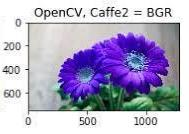
\includegraphics[width=2.5cm]{bgr.jpg}\\[2pt]
        \tiny Κανάλια: B, G, R
    };
    
    % RGB Box
    \node (rgb) at (7,0) [box, fill=red!15] {
        \textbf{Πλαίσιο RGB}\\[4pt]
        \small (Είσοδος MediaPipe)\\[4pt]
        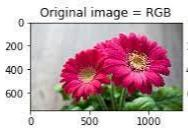
\includegraphics[width=2.5cm]{rgb.jpg}\\[2pt]
        \tiny Κανάλια: R, G, B
    };

    % Arrow
    \draw[->, ultra thick, draw=black!80] (bgr) -- node[above, font=\small] {\texttt{cvtColor()}} node[below, font=\tiny] {BGR2RGB} (rgb);

\end{tikzpicture}
\caption{Στιγμιότυπα επεξεργασίας εικόνας κατά τη μετατροπή από τον χρωματικό χώρο BGR σε RGB.}
\label{fig:bgr_to_rgb}
\end{figure}

Όπως φαίνεται στο Σχήμα~\ref{fig:bgr_to_rgb}, η σωστή μετατροπή των χρωματικών καναλιών είναι απαραίτητη για τη σωστή τροφοδοσία των αλγορίθμων υπολογιστικής όρασης.[15]

\subsubsection{Το Πλαίσιο Google MediaPipe και Αναγνώριση Σημείων}

Για τον εντοπισμό και την παρακολούθηση των χαρακτηριστικών του προσώπου σε πραγματικό χρόνο,
το σύστημα HorusAccess ενσωματώνει το πλαίσιο ανοικτού κώδικα Google MediaPipe και ειδικότερα τη
λύση MediaPipe Face Mesh. Το συγκεκριμένο εργαλείο βασίζεται σε αρχιτεκτονικές Βαθιάς Μάθησης
(Deep Learning) και παρέχει τη δυνατότητα χαρτογράφησης 468 τρισδιάστατων σημείων αναφοράς (3D
facial landmarks) στο ανθρώπινο πρόσωπο με υψηλή συχνότητα δειγματοληψίας.[16]

\begin{figure}[!htbp]
\centering
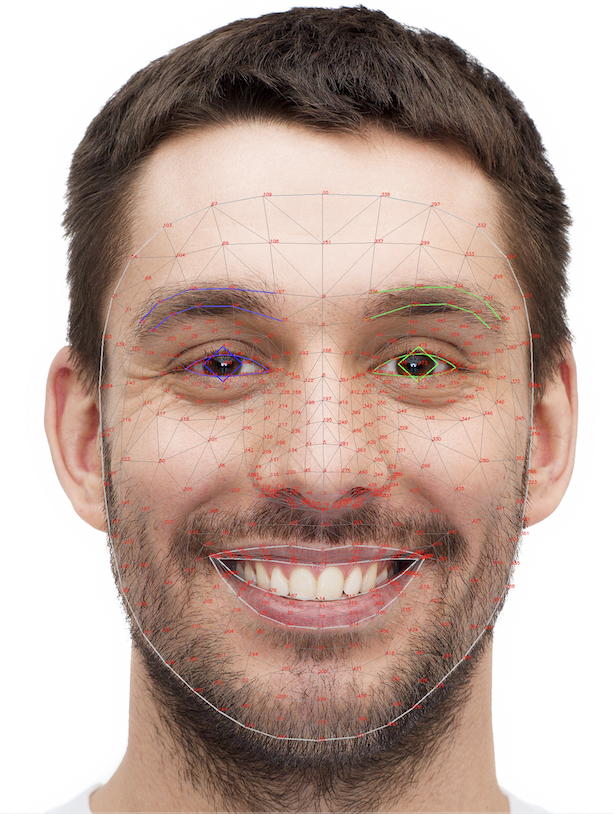
\includegraphics[width=0.35\textwidth]{face.png}
\caption{Χαρτογράφηση των τρισδιάστατων σημείων αναφοράς (facial landmarks) στο πρόσωπο μέσω του MediaPipe Face Mesh.}
\label{fig:mediapipe_face}
\end{figure}

Στο πεδίο της Μηχανικής Όρασης (Computer Vision), η εκπαίδευση (training) ενός Νευρωνικού Δικτύου ορίζεται ως η υπολογιστική διαδικασία κατά την οποία το μοντέλο τροφοδοτείται με τεράστιο
όγκο επισημειωμένων δεδομένων (annotated datasets — όπως εκατοντάδες χιλιάδες εικόνες προσώπων
με προκαθορισμένα σημεία). Κατά τη διάρκεια αυτής της φάσης, οι παράμετροι του δικτύου (βάρη και
πολώσεις / weights and biases) προσαρμόζονται επαναληπτικά μέσω αλγορίθμων βελτιστοποίησης (όπως
ο Stochastic Gradient Descent) και οπισθοδιάδοσης σφάλματος (backpropagation), ώστε το σύστημα να
μάθει να γενικεύει και να αναγνωρίζει μοτίβα σε άγνωστες εικόνες.[17]

Η εκπαίδευση ενός μοντέλου από το μηδέν (from scratch) καθίσταται απαραίτητη μόνο όταν το πρόβλημα αφορά ένα εξαιρετικά εξειδικευμένο πεδίο με μοναδικά χαρακτηριστικά δεδομένων, για τα οποία
δεν υφίστανται διαθέσιμα μοντέλα στη βιβλιογραφία, καθώς απαιτεί τεράστιους υπολογιστικούς πόρους
(πολλαπλές εξειδικευμένες μονάδες GPU/TPU), χρονοβόρα συλλογή και χειροκίνητη επισημείωση (labeling) δεδομένων, καθώς και παρατεταμένο χρόνο εκπαίδευσης. Αντιθέτως, μια προεκπαιδευμένη βιβλιοθήκη (pre-trained framework) περιλαμβάνει μοντέλα των οποίων τα βάρη έχουν ήδη βελτιστοποιηθεί
εκ των προτέρων από ερευνητικούς οργανισμούς σε γιγαντιαία σύνολα δεδομένων (large-scale datasets).

Για τους λόγους αυτούς, η υιοθέτηση του προεκπαιδευμένου πλαισίου MediaPipe έναντι της ανάπτυξης
και εκπαίδευσης ενός ιδιοταγούς μοντέλου κρίθηκε ακαδημαϊκά και τεχνικά επιβεβλημένη. Αφενός, διασφαλίζεται υψηλή γενικευσιμότητα και ανθεκτικότητα (robustness), καθώς το μοντέλο της Google έχει
εκπαιδευτεί σε εκατομμύρια εικόνες υπό ποικίλες συνθήκες φωτισμού, γωνίες λήψης, διαφορετικούς
τύπους προσώπων, ηλικίες και εθνικότητες, αποτρέποντας το φαινόμενο της υπερπροσαρμογής (overfitting). Αφετέρου, το MediaPipe είναι βελτιστοποιημένο για εκτέλεση σε πραγματικό χρόνο (real-time
edge inference) ενσωματώνοντας ελαφριές αρχιτεκτονικές (όπως MobileNet και BlazeFace), γεγονός που
επιτρέπει την τοπική εκτέλεση (on-device inference) στην Κεντρική Μονάδα Επεξεργασίας (CPU) του
συμβατικού υπολογιστή του χρήστη χωρίς να απαιτείται αυτόνομη κάρτα γραφικών (GPU). Επιπλέον, η
επιλογή αυτή επιτρέπει την εστίαση στην ουσιαστική καινοτομία της παρούσας διπλωματικής εργασίας,
συμπυκνώνοντας την προσπάθεια στο σχεδιασμό της αλληλεπίδρασης (HCI), στην ανάπτυξη των αλγορίθμων ελέγχου κέρσορα, στον υπολογισμό εκφράσεων και στη διασφάλιση της προσβασιμότητας, αντί
της ανάλωσης σε ένα ήδη επιλυμένο πρόβλημα ανίχνευσης προσώπου.[16,18]

Μετά την εξαγωγή των 3D συντεταγμένων $(x, y, z)$ των σημείων αναφοράς από το \textlatin{MediaPipe}, το σύστημα εκτελεί μαθηματική ανάλυση των γεωμετρικών μεταβολών σε πραγματικό χρόνο, ώστε να πραγματοποιηθεί η εξαγωγή χαρακτηριστικών και η αντιστοίχιση σε εντολές αλληλεπίδρασης.

\smallskip
\noindent\textbf{Υπολογισμός Ευκλείδειας Απόστασης:} Για την ανίχνευση των εκφράσεων, υπολογίζεται η Ευκλείδεια απόσταση μεταξύ δύο σημείων $P_1(x_1, y_1)$ και $P_2(x_2, y_2)$ στο επίπεδο της εικόνας:
\begin{equation}
d(P_1, P_2) = \sqrt{(x_2 - x_1)^2 + (y_2 - y_1)^2}
\end{equation}

Η παραπάνω σχέση εφαρμόζεται για τον ποσοτικό προσδιορισμό διαφόρων μορφολογικών μεταβολών και χαρακτηριστικών του προσώπου, τα οποία αναλύονται διεξοδικά παρακάτω:

\begin{itemize}
    \item \textbf{Μορφολογία Στόματος:} Όπως απεικονίζεται στο Σχήμα~\ref{fig:mouth_geometry}, η κατακόρυφη απόσταση μεταξύ των κεντρικών σημείων του άνω και κάτω χείλους ($p_2$ και $p_3$) υπολογίζει το εύρος ανοίγματος του στόματος, ενώ η οριζόντια απόσταση μεταξύ των άκρων/γωνιών του στόματος ($p_1$ και $p_4$) προσδιορίζει την έκταση του χαμόγελου ή της σύσπασης. Η γεωμετρική αυτή προσέγγιση αξιοποιείται ευρέως στην ανίχνευση συναισθημάτων και ομιλίας [19].
    
    \item \textbf{Οφθαλμική Δραστηριότητα:} Η σχέση των κατακόρυφων και οριζόντιων αποστάσεων στα βλέφαρα (Σχήμα~\ref{fig:facial_geometry}) επιτρέπει τον υπολογισμό του δείκτη κλεισίματος των οφθαλμών (\textlatin{Eye Aspect Ratio - EAR}) \cite{soukupova2016real}. Η μέτρηση αυτή διαχωρίζει με ακρίβεια το εκούσιο κλείσιμο (\textlatin{blink}) από το φυσιολογικό ανοιγόκλεισμα ή την κόπωση, βασιζόμενη στα πρότυπα εντοπισμού σημείων του \textlatin{MediaPipe Face Mesh} [18].
    
    \item \textbf{Κινητικότητα Φρυδιών:} Η μέση Ευκλείδεια απόσταση μεταξύ των σημείων των φρυδιών και των αντίστοιχων ορίων των οφθαλμών (Σχήμα~\ref{fig:eyebrow_geometry}) μεταφράζεται σε δυναμικές εντολές ανύψωσης (ένδειξη έκπληξης) ή συνοφρύωσης (ένδειξη θυμού ή συγκέντρωσης), ακολουθώντας τα πρότυπα κωδικοποίησης εκφράσεων \textlatin{FACS} (\textlatin{Facial Action Coding System}) [20].
\end{itemize}

\begin{figure}[!htbp]
\centering
\begin{tikzpicture}[scale=1.2]
    % Περίγραμμα στόματος (άνω και κάτω χείλος)
    \draw[thick, smooth, fill=red!5] plot coordinates {(-1.5,0) (-0.7,0.3) (0,0.35) (0.7,0.3) (1.5,0) (0.7,-0.4) (0,-0.45) (-0.7,-0.4) (-1.5,0)};
    
    % Σημεία αναφοράς (Γωνίες στόματος και κέντρα χειλιών)
    \filldraw [red] (-1.5,0) circle (2pt) node[left] {\scriptsize $p_1$ (Αριστερή Γωνία)};
    \filldraw [red] (1.5,0) circle (2pt) node[right] {\scriptsize $p_4$ (Δεξιά Γωνία)};
    \filldraw [red] (0,0.35) circle (2pt) node[above] {\scriptsize $p_2$ (Άνω Χείλος)};
    \filldraw [red] (0,-0.45) circle (2pt) node[below] {\scriptsize $p_3$ (Κάτω Χείλος)};
    
    % Αποστάσεις (Οριζόντια και Κατακόρυφη)
    \draw[dashed, blue, thick] (-1.5,0) -- (1.5,0);
    \draw[dashed, blue, thick] (0,0.35) -- (0,-0.45);
\end{tikzpicture}
\caption{Γεωμετρικός υπολογισμός μορφολογίας στόματος (οριζόντιο εύρος και κατακόρυφο άνοιγμα).}
\label{fig:mouth_geometry}
\end{figure}

\begin{figure}[!htbp]
\centering
\begin{tikzpicture}[scale=1.3]
    % Περίγραμμα ματιού (οβάλ / αμυγδαλωτό σχήμα)
    \draw[thick, smooth, tension=0.7, fill=gray!5] plot coordinates {(0,0) (1,0.45) (2,0.45) (3,0) (2,-0.45) (1,-0.45) (0,0)};
    
    % Ίριδα και κόρη ματιού για πιο ρεαλιστική απεικόνιση
    \filldraw [gray!30] (1.5,0) circle (0.45cm);
    \filldraw [black] (1.5,0) circle (0.2cm);
    
    % 6 Σημεία αναφοράς MediaPipe Face Mesh για EAR
    \filldraw [red] (0,0) circle (2pt) node[left] {\scriptsize $p_1$};
    \filldraw [red] (1,0.4) circle (2pt) node[above] {\scriptsize $p_2$};
    \filldraw [red] (2,0.4) circle (2pt) node[above] {\scriptsize $p_3$};
    \filldraw [red] (3,0) circle (2pt) node[right] {\scriptsize $p_4$};
    \filldraw [red] (2,-0.4) circle (2pt) node[below] {\scriptsize $p_5$};
    \filldraw [red] (1,-0.4) circle (2pt) node[below] {\scriptsize $p_6$};
    
    % Κατακόρυφες αποστάσεις (ύψος ματιού)
    \draw[dashed, blue, thick] (1,0.4) -- (1,-0.4);
    \draw[dashed, blue, thick] (2,0.4) -- (2,-0.4);
    
    % Οριζόντια απόσταση (πλάτος ματιού)
    \draw[dashed, red, thick] (0,0) -- (3,0);
\end{tikzpicture}
\caption{Αναλυτικός γεωμετρικός υπολογισμός του δείκτη EAR με χρήση 6 σημείων αναφοράς (MediaPipe) στον οφθαλμό.}
\label{fig:facial_geometry}
\end{figure}

\begin{figure}[!htbp]
\centering
\begin{tikzpicture}[scale=1.2]
    % Μάτι (αναφορά βάσης)
    \draw[thick, smooth, tension=0.7, fill=gray!5] plot coordinates {(0,0) (1,0.35) (2,0.35) (3,0) (2,-0.35) (1,-0.35) (0,0)};
    \filldraw [black] (1.5,0) circle (0.15cm);

    % Φρύδι (από πάνω)
    \draw[ultra thick, blue] (0.2,1.2) to[out=15,in=165] (2.8,1.2);
    
    % Σημεία μέτρησης απόστασης
    \filldraw [red] (1.5,0.35) circle (2pt) node[below=2pt] {\scriptsize $p_{\text{μάτι}}$};
    \filldraw [red] (1.5,1.2) circle (2pt) node[above=2pt] {\scriptsize $p_{\text{φρύδι}}$};
    
    % Κατακόρυφη απόσταση
    \draw[dashed, red, thick] (1.5,0.35) -- (1.5,1.2) node[midway, right, font=\tiny] {Απόσταση $d$};
\end{tikzpicture}
\caption{Μέτρηση απόστασης μεταξύ φρυδιού και οφθαλμού για την ανίχνευση κινητικότητας (ανύψωση/συνοφρύωση).}
\label{fig:eyebrow_geometry}
\end{figure}
\clearpage
\bigskip
\noindent\textbf{Αναλογικός Έλεγχος Κατεύθυνσης (\textlatin{Joystick Head Tracking}):} Για τη μετακίνηση του δείκτη στην οθόνη, ορίζεται ένα κεντρικό σημείο αναφοράς στο πρόσωπο, $P_{\text{nose}} = (x, y)$, και μια αρχική θέση ηρεμίας (κεντράρισμα), $P_{\text{neutral}} = (x_0, y_0)$. Η διανυσματική απόκλιση $\vec{D} = (\Delta x, \Delta y)$ υπολογίζεται ως:
\begin{equation}
\Delta x = x - x_0, \quad \Delta y = y - y_0
\end{equation}

Το μέτρο της μετατόπισης (εκτοπισμένο μήκος) ισούται με:
\begin{equation}
\|\vec{D}\| = \sqrt{\Delta x^2 + \Delta y^2}
\end{equation}

Για την αποφυγή ακούσιων μικρομετακινήσεων (\textlatin{tremor}), εισάγεται μια κατώφλια νεκρή ζώνη $r_{\text{dead}}$. Εάν $\|\vec{D}\| > r_{\text{dead}}$, η ενεργός μετατόπισις $e = \|\vec{D}\| - r_{\text{dead}}$ μετασχηματίζεται μη γραμμικά για τον υπολογισμό της ταχύτητας $V$ του κέρσορα:
\begin{equation}
V = S \cdot e^{\gamma}
\end{equation}
όπου $S$ είναι ο συντελεστής ευαισθησίας που ορίζεται από τον χρήστη και $\gamma > 1$ (π.χ. $\gamma = 1.5$) είναι ο εκθέτης μη γραμμικής επιτάχυνσης.

\begin{figure}[H]
\centering
\begin{tikzpicture}
    % Axes
    \draw[->, gray, thick] (-2.5,0) -- (2.5,0) node[right] {$X$};
    \draw[->, gray, thick] (0,-2.5) -- (0,2.5) node[above] {$Y$};
    
    % Deadzone Circle
    \draw[dashed, orange, thick, fill=orange!5] (0,0) circle (1.2cm);
    \node[orange!80!black] at (0.8,0.3) {\scriptsize $r_{\text{dead}}$};
    
    % Origin Neutral
    \filldraw [black] (0,0) circle (2pt) node[below left] {\scriptsize $P_{\text{neutral}}$};
    
    % Current Position Vector
    \filldraw [blue] (1.6,1.4) circle (2.5pt) node[above right] {\scriptsize $P_{\text{nose}}$};
    \draw[->, blue, thick] (0,0) -- (1.6,1.4) node[midway, above left] {\scriptsize $\vec{D}$};
\end{tikzpicture}
\caption{Σχηματική αναπαράσταση του μοντέλου Joystick Head Tracking και της νεκρής ζώνης ($r_{\text{dead}}$).}
\label{fig:joystick_deadzone}
\end{figure}

Όπως διαγράφεται στο Σχήμα~\ref{fig:joystick_deadzone}, η προσέγγιση αυτή επιτρέπει στον χρήστη να εκτελεί κινήσεις υψηλής ακρίβειας κοντά στο κέντρο (εντός των ορίων της νεκρής ζώνης), διατηρώντας παράλληλα τη δυνατότητα ταχείας διάσχισης της οθόνης σε μεγάλες εκτροπές της κεφαλής.

Οι παραπάνω γεωμετρικές τιμές και υπολογιζόμενες ταχύτητες συγκρίνονται συνεχώς με προσαρμοσμένα κατώφλια ευαισθησίας, επιτρέποντας τη διακριτοποίηση των ακούσιων φυσιολογικών κινήσεων από τις εσκεμμένες εντολές αλληλεπίδρασης.[19.20]
\subsection{Τεχνητή Νοημοσύνη}
Η Τεχνητή Νοημοσύνη (\textlatin{Artificial Intelligence - AI}) παρέχει το αντιληπτικό και γνωστικό υπόβαθρο 
για τη μοντελοποίηση τόσο της οπτικής πληροφορίας (\textlatin{Vision-based AI}) όσο και της φυσικής γλώσσας
(\textlatin{Natural Language Processing - NLP}). 
Στο πλαίσιο των σύγχρονων αρχιτεκτονικών, η τεχνητή νοημοσύνη αξιοποιεί μοντέλα Βαθιάς Μάθησης (\textlatin{Deep Learning}) τα οποία
βασίζονται σε πολυεπίπεδα τεχνητά νευρωνικά δίκτυα για την αυτόματη εξαγωγή μοτίβων και χαρακτηριστικών από ακατέργαστα δεδομένα 


Στο πεδίο της υπολογιστικής όρασης, η αυτόματη αναγνώριση και παρακολούθηση προσώπου 
βασίζεται στον συνδυασμό Συνελικτικών Νευρωνικών Δικτύων (\textlatin{Convolutional Neural Networks - CNNs}) και
 τεχνικών εκτίμησης γεωμετρικών σημείων (\textlatin{Landmark Estimation}). Η διαδικασία ξεκινά με ένα αρχικό δίκτυο ανίχνευσης
  (\textlatin{Object Detector}), το οποίο σαρώνει την εικόνα για τον εντοπισμό της περιοχής του προσώπου. 
  Το δίκτυο αυτό εφαρμόζει συνελικτικά φίλτρα για την εξαγωγή τοπικών χαρακτηριστικών, όπως ακμές και αντιθέσεις, 
  ορίζοντας τελικά την Περιοχή Ενδιαφέροντος (\textlatin{Region of Interest - ROI}). Στη συνέχεια, ένα εξειδικευμένο 
  βαθύ συνελικτικό δίκτυο δέχεται ως είσοδο την περιοχή αυτή και εκτελεί παλινδρόμηση για την πρόβλεψη των τρισδιάστατων 
  συντεταγμένων $\mathbf{P} = \{(x_i, y_i, z_i)\}_{i=1}^{K}$ για ένα πυκνό σύνολο $K$ χαρακτηριστικών σημείων (\textlatin{landmarks}).

Η μαθηματική απεικόνιση της εικόνας εισόδου $\mathbf{I} \in \mathbb{R}^{W \times H \times C}$, όπου $W$ και $H$ είναι οι διαστάσεις και $C$ τα χρωματικά κανάλια, στον χώρο των $K$ σημείων εκφράζεται ως:
\begin{equation}
\mathbf{P} = f_{\theta}(\mathbf{I})
\end{equation}
όπου $f_{\theta}$ συμβολίζει το νευρωνικό δίκτυο με εκπαιδευμένες παραμέτρους (βάρη) $\theta$. Η συντεταγμένη $z_i$ εκτιμάται σχεσιακά, αντιπροσωπεύοντας το σχετικό βάθος του σημείου ως προς το κέντρο μάζας του προσώπου.[21]

Προκειμένου να διατηρηθεί υψηλή υπολογιστική αποδοτικότητα και χαμηλή καθυστέρηση (\textlatin{latency}), η διαδικασία χωρίζεται σε δύο διακριτές φάσεις: τη φάση ανίχνευσης και τη φάση παρακολούθησης (\textlatin{tracking}) \cite{lugaresi2019mediapipe}. Στη φάση παρακολούθησης, το δίκτυο χρησιμοποιεί τις θέσεις των σημείων του προηγούμενου καρέ για να προβλέψει τις νέες θέσεις στο τρέχον καρέ. Η επαναφορά της απαιτητικής διαδικασίας πλήρους ανίχνευσης ενεργοποιείται μόνο όταν ο δείκτης βεβαιότητας (\textlatin{confidence score} $c \in [0,1]$) του δικτύου πέσει κάτω από ένα ορισμένο κατώφλι αξιοπιστίας $c_{\text{thresh}}$:
\begin{equation}
\text{Mode} = \begin{cases} 
\text{Tracking}, & \text{εάν } c \ge c_{\text{thresh}} \\ 
\text{Detection}, & \text{εάν } c < c_{\text{thresh}} 
\end{cases}
\end{equation}

Παράλληλα με την οπτική αντιληπτική ικανότητα, τα Μεγάλα Γλωσσικά Μοντέλα (\textlatin{Large Language Models - LLMs}) αποτελούν την αιχμή του δόρατος στην Επεξεργασία Φυσικής Γλώσσας, επιτρέποντας στα υπολογιστικά συστήματα να κατανοούν, να παράγουν και να μετασχηματίζουν τον ανθρώπινο λόγο. Η δομική λίθος των σύγχρονων γλωσσικών μοντέλων είναι η αρχιτεκτονική \textlatin{Transformer} \cite{vaswani2017attention}. Η θεμελιώδης καινοτομία των \textlatin{Transformers} έγκειται στον μηχανισμό αυτο-προσοχής (\textlatin{Self-Attention}), ο οποίος επιτρέπει στο μοντέλο να σταθμίζει τη σημασία κάθε λέξης (\textlatin{token}) σε σχέση με όλες τις άλλες λέξεις της πρότασης, ανεξάρτητα από τη μεταξύ τους απόσταση.

Για μια ακολουθία εισόδου, υπολογίζονται τα διανύσματα Ερωτήματος ($Q$), Κλειδιού ($K$) και Τιμής ($V$). Η συνάρτηση προσοχής ορίζεται μαθηματικά ως \cite{vaswani2017attention}:
\begin{equation}
\text{Attention}(Q, K, V) = \text{softmax}\left(\frac{QK^T}{\sqrt{d_k}}\right)V
\end{equation}
όπου $d_k$ είναι η διάσταση των διανυσμάτων κλειδιού, ενώ ο παράγοντας $\sqrt{d_k}$ χρησιμοποιείται για τη διατήρηση της ευστάθειας των παραγώγων κατά τη διάρκεια της εκπαιδευσης.

Σε θεωρητικό επίπεδο, ένα γλωσσικό μοντέλο εκπαιδεύεται να υπολογίζει την κατανομή πιθανότητας μιας ακολουθίας συμβόλων $W = (w_1, w_2, \dots, w_n)$. Η πιθανότητα ολόκληρης της ακολουθίας αναλύεται στο γινόμενο των δεσμευμένων πιθανοτήτων κάθε συμβόλου, δοθέντων των προηγούμενων συμβόλων:
\begin{equation}
P(W) = \prod_{i=1}^{n} P(w_i \mid w_1, w_2, \dots, w_{i-1})
\end{equation}

Στο πλαίσιο των αυτόνομων συστημάτων αλληλεπίδρασης, τα Μεγάλα Γλωσσικά Μοντέλα δεν περιορίζονται στην παραγωγή ελεύθερου κειμένου. Μέσω τεχνικών ευθυγράμμισης (\textlatin{alignment}) και ειδικής εκπαίδευσης προσαρμογής σε εντολές (\textlatin{instruction tuning}), τα μοντέλα αποκτούν την ικανότητα να λειτουργούν ως μεταφραστές προθέσεων (\textlatin{Intent Translators}). Όταν το μοντέλο λάβει μια πρόταση φυσικής γλώσσας (προερχόμενη από μετατροπή ομιλίας σε κείμενο μέσω αλγορίθμων \textlatin{Speech-to-Text}), αναλύει τη σημασιολογία της και την αντιστοιχίζει σε μια δομημένη αναπαράσταση.

Η διαδικασία αυτή περιλαμβάνει αρχικά την αναγνώριση της πρόθεσης (\textlatin{Intent Classification}) για τον προσδιορισμό της επιθυμίας του χρήστη, στη συνέχεια την εξαγωγή παραμέτρων (\textlatin{Slot Filling}) για τον εντοπισμό των συγκεκριμένων μεταβλητών, και τέλος την παραγωγή δομημένης εξόδου (\textlatin{Structured Output Generation}). Με τον μετασχηματισμό του αποτελέσματος σε αυστηρά δομημένη μορφή (όπως συμβολοσειρές \textlatin{JSON}), επιτυγχάνεται η γεφύρωση του χάσματος μεταξύ της ασαφούς φυσικής γλώσσας και των αυστηρά καθορισμένων διεπαφών προγραμματισμού των λογισμικών.[22]

\subsubsection{Αρχιτεκτονική Ενσωμάτωσης Μοντέλων μέσω Ollama}

Το \textlatin{Ollama} είναι ένα ανοικτού κώδικα λογισμικό που σχεδιάστηκε για να απλοποιεί την εκτέλεση και διαχείριση Μεγάλων Γλωσσικών Μοντέλων (\textlatin{LLMs}) τοπικά σε προσωπικούς υπολογιστές \cite{ollama2023}. Στο πλαίσιο του συστήματος, η τοπική εκτέλεση πραγματοποιείται μέσω του εν λόγω πλαισίου, το οποίο παρέχει μια ελαφριά, βελτιστοποιημένη υποδομή εκτέλεσης (\textlatin{inference engine}) βασισμένη στη βιβλιογραφία του \textlatin{llama.cpp}, επιτρέποντας την αποτελεσματική αξιοποίηση των πόρων του συστήματος (τόσο στην Κεντρική Μονάδα Επεξεργασίας — \textlatin{CPU}, όσο και σε διαθέσιμες μονάδες \textlatin{GPU}) χωρίς την εξάρτηση από εξωτερικές υπηρεσίες υπολογιστικού νέφους (\textlatin{Cloud APIs}).

\paragraph{Ποσοτικοποίηση Μοντέλων (\textlatin{Model Quantization})}
Για τη διασφάλιση χαμηλής κατανάλωσης μνήμης (\textlatin{RAM/VRAM}) και τη διατήρηση υψηλής ταχύτητας απόκρισης σε συμβατικό εξοπλισμό, το πλαίσιο αξιοποιεί τεχνικές ποσοτικοποίησης (\textlatin{quantization}). Κατά τη διαδικασία αυτή, οι παράμετροι $\theta$ του γλωσσικού μοντέλου, οι οποίες αρχικά εκπροσωπούνται σε μορφή κινητής υποδιαστολής υψηλής ακρίβειας (\textlatin{FP16} ή \textlatin{FP32}), μετασχηματίζονται σε αναπαραστάσεις χαμηλότερης βηματικής ακρίβειας (όπως \textlatin{INT8} ή \textlatin{INT4}).

Μαθηματικά, μια παράμετρος κινητής υποδιαστολής $w \in \mathbb{R}$ χαρτογραφείται σε μια ακέραια τιμή $q \in [-2^{b-1}, 2^{b-1}-1]$ με εύρος $b$ bits μέσω της συνάρτησης:
\begin{equation}
q = \text{round}\left( \frac{w}{S} \right) + Z
\end{equation}
όπου $S$ είναι ο συντελεστής κλίμακας (\textlatin{scale factor}) και $Z$ το σημείο μηδενισμού (\textlatin{zero-point}). Η προσέγγιση αυτή επιτυγχάνει δραστική μείωση του αποτυπώματος μνήμης και επιταχύνει τους υπολογισμούς, διατηρώντας παράλληλα την ποιότητα και τη σημασιολογική πιστότητα των παραγόμενων απαντήσεων.

\paragraph{Επικοινωνία μέσω \textlatin{REST API} και Δομημένη Έξοδος}
Η διασύνδεση του συστήματος με το πλαίσιο \textlatin{Ollama} πραγματοποιείται μέσω ασύγχρονων αιτημάτων \textlatin{HTTP REST API}. Το κύριο πρόγραμμα αποστέλλει το κείμενο εισόδου (συμπεριλαμβανομένου του κατάλληλου προτύπου οδηγιών / \textlatin{system prompt}) στη διαδρομή \textlatin{/api/generate} ή \textlatin{/api/chat}.

Προκειμένου να διασφαλιστεί η παραγωγή αυστηρά δομημένης εξόδου (\textlatin{Structured JSON Output}) για την εξαγωγή προθέσεων (\textlatin{Intent Classification}) και παραμέτρων (\textlatin{Slot Filling}), η κλήση συνοδεύεται από τον ορισμό σχήματος (\textlatin{JSON Schema constraint}). Το μοντέλο περιορίζει το χώρο δειγματοληψίας των συμβόλων (\textlatin{tokens}) αποκλειστικά σε έγκυρες δομές \textlatin{JSON}, αποτρέποντας την εισαγωγή ελεύθερου κειμένου ή απρόβλεπτων συμβόλων.[24]

\paragraph{Πλεονεκτήματα Τοπικής Εκτέλεσης}
Η αρχιτεκτονική επιλογή του \textlatin{Ollama} για τη διπλωματική εργασία προσφέρει σημαντικά πλεονεκτήματα:
\begin{itemize}
    \item \textbf{Ιδιωτικότητα και Ασφάλεια Δεδομένων (\textlatin{Data Privacy}):} Η επεξεργασία της ομιλίας και του κειμένου του χρήστη εκτελείται εξ ολοκλήρου τοπικά (\textlatin{on-device}), χωρίς τη μεταφορά ευαίσθητων προσωπικών δεδομένων σε τρίτους παρόχους.
    \item \textbf{Μηδενικό Κόστος Χρήσης και Ανεξαρτησία Δικτύου:} Διασφαλίζεται η απρόσκοπτη λειτουργία του συστήματος ακόμη και σε περιβάλλοντα χωρίς σύνδεση στο διαδίκτυο (\textlatin{offline mode}), εξαλείφοντας παράλληλα το λειτουργικό κόστος ανά κλήση (\textlatin{pay-per-token}).
    \item \textbf{Προβλέψιμη Καθυστέρηση (\textlatin{Low Latency}):} Αποφεύγονται οι καθυστερήσεις δικτύου (\textlatin{network latency}) και οι διακυμάνσεις απόκρισης των εξωτερικών εξυπηρετητών, προσφέροντας άμεση αλληλεπίδραση στον χρήστη.
\end{itemize}

\subsection{Αλληλεπίδραση Ανθρώπου-Υπολογιστή}
Η Αλληλεπίδραση Ανθρώπου-Υπολογιστή (\textlatin{Human-Computer Interaction - HCI}) στο πεδίο της προσβασιμότητας εστιάζει στον σχεδιασμό διεπαφών που ελαχιστοποιούν το γνωστικό και σωματικό φορτίο του χρήστη, 
λαμβάνοντας υπόψη τις ιδιαίτερες ανάγκες ατόμων με κινητικές ή αισθητηριακές αναπηρίες [3]. Στο πλαίσιο αυτό, η επιλογή των σχεδιαστικών αρχών, της οπτικής εργονομίας και των μηχανισμών υποβοήθησης βασίζεται
σε θεμελιώδη θεωρητικά υπόβαθρα της επιστήμης υπολογιστών, της γνωστικής ψυχολογίας και της σχεδίασης χωρίς αποκλεισμούς (\textlatin{Inclusive Design}), με στόχο τη βελτιστοποίηση της χρηστικότητας, της ακρίβειας και της ταχύτητας αλληλεπίδρασης.[25]

Όσον αφορά την οπτική σχεδίαση της διεπαφής (\textlatin{Visual UX design}), η υιοθέτηση ενός σκοτεινού θέματος (\textlatin{Dark Mode}) με στοιχεία υψηλής αντίθεσης (\textlatin{High Contrast}) σε φωτεινές γαλαζοπράσινες 
αποχρώσεις βασίζεται τόσο στη θεωρία της αισθητηριακής εργονομίας όσο και στις αρχές της ψυχοκοινωνικής συμπεριληπτικότητας. Από τεχνική και φυσιολογική σκοπιά, η επιλογή αυτή μειώνει τη συνολική φωτεινότητα της οθόνης, 
περιορίζοντας την οφθαλμική κόπωση (\textlatin{eye strain}) που προκαλείται από την παρατεταμένη έκθεση σε λευκά υπόβαθρα, ιδιαίτερα για χρήστες που αλληλεπιδρούν μέσω κινήσεων του προσώπου. Παράλληλα, οι έντονες χρωματικές αντιθέσεις 
δημιουργούν σαφή διαχωρισμό μεταξύ των ενεργών στοιχείων και του υποβάθρου, ενισχύοντας την οπτική αναγνωρισιμότητα (\textlatin{visual saliency}) και επιτρέποντας την ταχεία εστίαση της προσοχής.[26]

Σε ψυχολογικό και κοινωνικό επίπεδο, η αισθητική αυτή προσέγγιση εξυπηρετεί έναν θεμελιώδη στόχο του συμπεριληπτικού σχεδιασμού: την αποφυγή του «στιγματιστικού» χαρακτήρα που συχνά φέρουν τα παραδοσιακά λογισμικά προσβασιμότητας. 
Υιοθετώντας μια σύγχρονη οπτική ταυτότητα (\textlatin{visual identity}) που παραπέμπει σε επαγγελματικά περιβάλλοντα ελέγχου και δημοφιλείς διεπαφές υψηλής απόδοσης (\textlatin{gaming interfaces}), 
η εφαρμογή προσφέρει μια εμπειρία χρήσης που δεν διαχωρίζει τον χρήστη λόγω της αναπηρίας του, αλλά του παρέχει ένα περιβάλλον ισότιμο, ελκυστικό και αισθητικά εναρμονισμένο με τις σύγχρονες τεχνολογικές τάσεις.

Στο επίπεδο της γεωμετρίας των διαδραστικών στοιχείων, ο σχεδιασμός κουμπιών με διευρυμένα όρια (\textlatin{large targets}) διέπεται αυστηρά από τον Νόμο του \textlatin{Fitts} (\textlatin{Fitts's Law}) \cite{fitts1954information, soukoreff2004fitts}. Στο πλαίσιο αυτό, ο χρόνος $T$ που απαιτείται για τη μετακίνηση του δείκτη σε μια περιοχή-στόχο είναι συνάρτηση της απόστασης $D$ από τον στόχο και του πλάτους $W$ του στόχου:
\begin{equation}
T = a + b \log_2 \left(1 + \frac{D}{W}\right)
\end{equation}
όπου $a$ και $b$ είναι εμπειρικές σταθερές \cite{soukoreff2004fitts}. Αυξάνοντας το πλάτος $W$ των κουμπιών, ελαττώνεται ο δείκτης δυσκολίας της κίνησης. Αυτό είναι καθοριστικής σημασίας για χρήστες με κινητικές αναπηρίες ή μειωμένο μυϊκό έλεγχο, καθώς μειώνει δραστικά την πιθανότητα σφάλματος και τον χρόνο απόκρισης κατά την επιλογή.[27]

Για την περαιτέρω διευκόλυνση της πλοήγησης, η ενσωμάτωση αλγορίθμων «μαγνητισμού» του κέρσορα (\textlatin{Magnetic Snap / Sticky Targets}) εισάγει την έννοια των εικονικών πεδίων δυναμικού (\textlatin{Virtual Potential Fields}) γύρω από τα διαδραστικά στοιχεία. 
Όταν ο κέρσορας εισέλθει στην περιοχή επιρροής ενός στόχου, το σύστημα ασκεί μια εικονική «έλξη» προς το κέντρο του. Στη θεωρία HCI, η τεχνική αυτή μετασχηματίζει τον φυσικό χώρο αλληλεπίδρασης, αυξάνοντας τεχνητά το αποτελεσματικό μέγεθος του στόχου ($W$) χωρίς να αλλοιώνει τη γραφική 
εμφάνιση της οθόνης, εξαλείφοντας έτσι τον ακούσιο τρόμο (\textlatin{micro-tremors}) των χρηστών.

\begin{figure}[!htbp]
\centering
\begin{tikzpicture}[scale=1]
    % Στόχος (Button)
    \draw[thick, fill=blue!10, rounded corners=5pt] (2,-1) rectangle (5,1);
    \node at (3.5,0) {\textbf{Στόχος}};
    
    % Πεδίο Μαγνητισμού (Magnetic Field Boundary - dashed)
    \draw[dashed, red, thick] (3.5,0) circle (2.2cm);
    \node[red!80!black, font=\scriptsize] at (3.5,1.9) {Πεδίο ``Μαγνητισμού'' ($W_{effective}$)};
    
    % Διαδρομή δείκτη με tremor (ακούσιες κινήσεις)
    \draw[blue, thick, decorate, decoration={random steps,segment length=3pt,amplitude=2pt}] 
        (0,-2) -- (1.5,-0.5) -- (2.8,0.2);
        
    % Σημείο έλξης (Snap)
    \draw[->, orange, ultra thick] (2.8,0.2) -- (3.5,0);
    
    % Σημεία
    \filldraw[blue] (0,-2) circle (2pt) node[below left] {\scriptsize Αρχική Θέση};
    \filldraw[black] (3.5,0) circle (2.5pt) node[above right] {\scriptsize Κέντρο Στόχου};
\end{tikzpicture}
\caption{Σχηματική απεικόνιση της λειτουργίας μαγνητισμού του κέρσορα (Magnetic Snap) γύρω από ένα διαδραστικό στοιχείο, η οποία αυξάνει το αποτελεσματικό πλευρικό μέγεθος ($W$) για τον περιορισμό του σφάλματος.}
\label{fig:magnetic_snap}
\end{figure}


Παράλληλα, η δυνατότητα προσαρμογής και αποθήκευσης της συμπεριφοράς του συστήματος σε πολλαπλά προφίλ χρήσης βασίζεται στις αρχές της προσαρμοστικότητας (\textlatin{Adaptability}) και της εξατομίκευσης (\textlatin{Personalization}). Καθώς οι φυσιολογικές δυνατότητες, 
η κόπωση ή το περιβάλλον αλληλεπίδρασης μεταβάλλονται, η διαμόρφωση διακριτών παραμέτρων επιτρέπει στο σύστημα να ανταποκρίνεται στις μεταβαλλόμενες ανάγκες του χρήστη, διατηρώντας σταθερό το επίπεδο αυτονομίας του.

Τέλος, η πολυτροπική αλληλεπίδραση (\textlatin{Multimodal Interaction}) μέσω της συνδυαστικής χρήσης οπτικών/κινητικών μέσων, φωνητικών εντολών και ενσωματωμένων οδηγιών χρήσης, στοχεύει στη βελτιστοποίηση του Γνωστικού Φορτίου (\textlatin{Cognitive Load Theory}). 
Η ταυτόχρονη ύπαρξη σαφών, άμεσα προσβάσιμων οδηγιών μειώνει τη μνημονική επιβάρυνση (\textlatin{working memory load}), 
ενισχύοντας την ευχρηστία και την αυτοπεποίθηση του χρήστη κατά την αλληλεπίδραση με το σύστημα.[28]



\subsection{Σύνοψη κεφαλαίου}
Στο παρόν κεφάλαιο παρουσιάστηκε το θεωρητικό, επιστημονικό και τεχνολογικό υπόβαθρο πάνω στο οποίο στηρίχθηκε ο σχεδιασμός του συστήματος \textlatin{HorusAccess}. Η ανάλυση κάλυψε τους τρεις θεμελιώδεις πυλώνες στους οποίους βασίζεται η λειτουργία της εφαρμογής, προσφέροντας μια ολοκληρωμένη επισκόπηση των αλγορίθμων, των μοντέλων και των αρχών σχεδίασης.

Αρχικά, εξετάστηκε ο τομέας της Επεξεργασίας Εικόνας, αναλύοντας τις θεωρητικές μεθόδους λήψης, προετοιμασίας και μετασχηματισμού της οπτικής ροής, καθώς και τη μαθηματική μοντελοποίηση των Ευκλείδειων αποστάσεων και διανυσματικών μετατοπίσεων για τον αναλογικό έλεγχο κατεύθυνσης και την ανίχνευση μορφολογικών μεταβολών του προσώπου. Στη συνέχεια, παρουσιάστηκε το πεδίο της Τεχνητής Νοημοσύνης, εστιάζοντας στις αρχιτεκτονικές Βαθιάς Μάθησης για την εκτίμηση τρισδιάστατων πλεγμάτων προσώπου (\textlatin{Face Mesh}), στις τεχνικές βελτιστοποίησης της παρακολούθησης (\textlatin{Tracking vs Detection}), καθώς και στη θεωρητική θεμελίωση των Μεγάλων Γλωσσικών Μοντέλων (\textlatin{LLMs}) και του μηχανισμού αυτο-προσοχής (\textlatin{Self-Attention}) για την κατανόηση προθέσεων φυσικής γλώσσας. Τέλος, αναλύθηκαν οι αρχές της Αλληλεπίδρασης Ανθρώπου-Υπολογιστή και του Συμπεριληπτικού Σχεδιασμού (\textlatin{Inclusive Design}), θεμελιώνοντας επιστημονικά τη χρήση του Νόμου του \textlatin{Fitts}, των εικονικών πεδίων δυναμικού για τον «μαγνητισμό» του κέρσορα, του σκοτεινού θέματος υψηλής αντίθεσης για τη μείωση του κοινωνικού στίγματος και της οφθαλμικής κόπωσης, καθώς και της πολυτροπικότητας για τη διαχείριση του γνωστικού φορτίου.

Η θεωρητική αυτή θεμελίωση καθιστά σαφές το επιστημονικό υπόβαθρο που απαιτείται για την ανάπτυξη μιας ανέπαφης, αυτόνομης και προσβάσιμης διεπαφής. Παράλληλα, θέτει τις απαραίτητες βάσεις για το επόμενο κεφάλαιο, όπου θα αναλυθεί η αρχιτεκτονική σχεδίαση και η πρακτική υλοποίηση του συστήματος \textlatin{HorusAccess}.

\clearpage
\section{Ανάλυση Απαιτήσεων και Σχεδίαση συστήματος}

\subsection{Εισαγωγή}
​Στο παρόν κεφάλαιο παρουσιάζεται η συστηματική ανάλυση των απαιτήσεων και ο αρχιτεκτονικός σχεδιασμός του συστήματος HorusAccess. Μετά τη θεμελίωση του θεωρητικού και τεχνολογικού υποβάθρου στο προηγούμενο κεφάλαιο, το ενδιαφέρον μετατοπίζεται στις δομικές, λειτουργικές και αλγοριθμικές προδιαγραφές που καθορίζουν τη συγκρότηση, τη συμπεριφορά και την οργάνωση του λογισμικού πριν από τη φάση της τεχνικής του υλοποίησης.
​Αρχικά, πραγματοποιείται η δομημένη καταγραφή και κατηγοριοποίηση των απαιτήσεων του συστήματος σε λειτουργικές (Functional Requirements) και μη λειτουργικές (Non-Functional Requirements). Οι λειτουργικές απαιτήσεις ορίζουν τις διακριτές δυνατότητες και υπηρεσίες που παρέχει η εφαρμογή, ενώ οι μη λειτουργικές προδιαγραφές θέτουν τα ποιοτικά κριτήρια, όπως η απόκριση σε πραγματικό χρόνο, η αξιοπιστία, η προσβασιμότητα και η υπολογιστική αποδοτικότητα.
​Στη συνέχεια, αναλύεται η συνολική αρχιτεκτονική του συστήματος (System Architecture) και τα διαγράμματα συμπεριφοράς (Use Cases), παρουσιάζοντας τη δομή των επιμέρους υποσυστημάτων, τη ροή δεδομένων και τις αρχές που εξασφαλίζουν τη δομοστοιχειωσιμότητα και την επεκτασιμότητα του λογισμικού. Παράλληλα, θεμελιώνεται το αλγοριθμικό πλαίσιο σχεδιασμού των κινήσεων, περιγράφοντας τα μαθηματικά μοντέλα μετατροπής των ανατομικών δεικτών του προσώπου σε αναλογικές και διακριτές εντολές αλληλεπίδρασης. Τέλος, παρουσιάζονται οι σχεδιαστικές αρχές του περιβάλλοντος αλληλεπίδρασης (UI/UX) με βάση κανόνες προσβασιμότητας και αισθητηριακής εργονομίας, θέτοντας τις βάσεις για την τεχνική υλοποίηση που ακολουθεί στο επόμενο κεφάλαιο.[29]

\subsection{Καταγραφή απαιτήσεων συστήματος}
​Η συστηματική καταγραφή και ανάλυση των απαιτήσεων αποτελεί τον θεμέλιο λίθο της διαδικασίας σχεδιασμού του συστήματος HorusAccess, 
καθώς καθορίζει το λειτουργικό εύρος, τις τεχνικές προδιαγραφές και τα ποιοτικά κριτήρια που διέπουν τη συμπεριφορά του λογισμικού. 
Δεδομένου ότι η εφαρμογή σχεδιάστηκε με πρωταρχικό στόχο την παροχή πλήρους ψηφιακής αυτονομίας σε άτομα με σοβαρές κινητικές αναπηρίες, 
η συλλογή των απαιτήσεων επικεντρώθηκε στην εξάλειψη των φυσικών εμποδίων αλληλεπίδρασης, στην ελαχιστοποίηση του μυϊκού και γνωστικού φορτίου, καθώς και στη διασφάλιση υψηλής αξιοπιστίας σε συνθήκες καθημερινής χρήσης. 
Για την πληρέστερη ακαδημαϊκή θεμελίωση και τη διασφάλιση της ιχνηλασιμότητας (traceability) του σχεδιασμού, οι προδιαγραφές κατηγοριοποιούνται σε Λειτουργικές Απαιτήσεις (Functional Requirements - FR) και Μη Λειτουργικές Απαιτήσεις (Non-Functional Requirements - NFR).[30]

\subsubsection{Καταγραφή λειτουργικών απαιτήσεων}
Οι λειτουργικές απαιτήσεις ορίζουν τις συγκεκριμένες δυνατότητες, τις αλληλεπιδράσεις και τις υπηρεσίες που οφείλει να παρέχει το σύστημα στον χρήστη.
Στον πυρήνα του λογισμικού βρίσκεται ο μηχανισμός ανέπαφου αναλογικού ελέγχου του δείκτη, ο οποίος αναλύει τη σχετική μετατόπιση της κεφαλής μέσω μιας τυπικής συσκευής λήψης βίντεο και τη μεταφράζει σε ακριβή κίνηση του κέρσορα στην οθόνη [31]. 
Παράλληλα, ενσωματώνεται μηχανισμός αναγνώρισης μορφολογικών μεταβολών του προσώπου σε πραγματικό χρόνο [FR-02]. Μέσω του υπολογισμού γεωμετρικών δεικτών, όπως ο λόγος πλευρικής προς κατακόρυφη απόσταση βλεφάρων (\textlatin{Eye Aspect Ratio - EAR}) και ο λόγος ανοίγματος στόματος (\textlatin{Mouth Open Ratio - MOR}), το σύστημα ανιχνεύει διακριτικές εκφράσεις (στιγμιαίος βλεφαρισμός, άνοιγμα στόματος) και τις αντιστοιχίζει σε συμβάντα ποντικιού.

Για την ελαχιστοποίηση της πολυπλοκότητας κατά τη ρύθμιση της εφαρμογής, το σύστημα ενσωματώνει τη μονάδα \textlatin{Horus AI} [FR-03], η οποία αξιοποιεί Μεγάλα Γλωσσικά Μοντέλα (\textlatin{Large Language Models - LLMs}) για την αυτόματη παραμετροποίηση του προφίλ αλληλεπίδρασης. 
Η μονάδα αυτή ανιχνεύει τα εγκατεστημένα παιχνίδια στον υπολογιστή του χρήστη, αναλύει τις απαιτήσεις του εκάστοτε τίτλου και παράγει αυτόματα βέλτιστες προτάσεις αντιστοίχισης κινήσεων και χειρονομιών, εξαλείφοντας την ανάγκη για χρονοβόρα χειροκίνητη πλοήγηση σε μενού ρυθμίσεων [32]. 
Επιπλέον, παρέχεται υψηλός βαθμός εξατομίκευσης μέσω της γενικότερης διαχείρισης προφίλ χρήσης [FR-04], διασφαλίζοντας ότι διαφορετικοί χρήστες ή ο ίδιος ο χρήστης υπό συνθήκες κόπωσης μπορούν να αποθηκεύουν, να επισκοπούν και να ανακαλούν τις προσωπικές τους ρυθμίσεις ευαισθησίας.

Για λόγους ασφαλείας, ενσωματώνεται μηχανισμός παράκαμψης,[FR-05] ο οποίος αναστέλλει προσωρινά τον αυτόματο έλεγχο όταν εντοπίζεται φυσική κίνηση από εξωτερικές περιφερειακές συσκευές, επιτρέποντας σε έναν φροντιστή να αναλάβει τον έλεγχο [31].
Τέλος, η αυτόνομη εισαγωγή κειμένου επιτυγχάνεται μέσω ενσωματωμένου εικονικού πληκτρολογίου βελτιστοποιημένου κατά τον Νόμο του \textlatin{Fitts} [33], ενώ οι παραγόμενες εντολές διοχετεύονται σε χαμηλό επίπεδο λειτουργικού συστήματος 
για διασφάλιση πλήρους συμβατότητας με τρίτες εφαρμογές.[33]

\begin{table}[!htbp]
\centering
\begin{tabular}{|l|p{4cm}|p{6.5cm}|}
\hline
\textbf{Κωδικός} & \textbf{Κατηγορία / Λειτουργία} & \textbf{Περιγραφή / Σκοπός} \\ \hline
\textbf{[FR-01]} & Αναλογικός Έλεγχος Δείκτη & Ανεπαφής έλεγχος κέρσορα μέσω μετατόπισης της κεφαλής από κάμερα. \\ \hline
\textbf{[FR-02]} & Ανίχνευση Εκφράσεων Προσώπου & Υπολογισμός \textlatin{EAR} και \textlatin{MOR} για αντιστοίχιση εκφράσεων σε κλικ. \\ \hline
\textbf{[FR-03]} & Αυτόματη Παραμετροποίηση (\textlatin{Horus AI}) & Χρήση \textlatin{LLMs} για ανίχνευση παιχνιδιών και αυτόματη ρύθμιση προφίλ. \\ \hline
\textbf{[FR-04]} & Διαχείριση Προφίλ & Αποθήκευση, επισκόπηση και ανάκληση εξατομικευμένων ρυθμίσεων. \\ \hline
\textbf{[FR-05]} & Παράκαμψη Ελέγχου (\textlatin{Override}) & Αναστολή αυτόματου ελέγχου σε περίπτωση φυσικής κίνησης από φροντιστή. \\ \hline
\textbf{[FR-06]} & Εικονικό Πληκτρολόγιο & Αυτόνομη εισαγωγή κειμένου βελτιστοποιημένη κατά τον Νόμο του \textlatin{Fitts}. \\ \hline
\textbf{[FR-07]} & Διοχέτευση Εντολών \textlatin{OS} & Ενσωμάτωση σε χαμηλό επίπεδο λειτουργικού για συμβατότητα εφαρμογών. \\ \hline
\end{tabular}
\caption{Συνοπτικός πίνακας λειτουργικών απαιτήσεων του συστήματος \textlatin{HorusAccess}.}
\label{tab:fr_summary}
\end{table}

\clearpage

\begin{figure}[!htbp]
\centering
\begin{tikzpicture}[>=stealth, node distance=2cm]
    % System Boundary (Πλαίσιο Συστήματος)
    \draw[thick, rounded corners=5pt, fill=gray!5] (-1, 3.5) rectangle (7.5, -5.5);
    \node[above, font=\bfseries] at (3.25, 3.5) {Σύστημα HorusAccess};

    % Use Cases (Ελλείψεις)
    \node[draw, ellipse, fill=white, minimum width=2.6cm, minimum height=1.0cm, align=center, font=\scriptsize] (fr1) at (1.5, 2) {[FR-01] Αναλογικός\\Έλεγχος Δείκτη};
    \node[draw, ellipse, fill=white, minimum width=2.6cm, minimum height=1.0cm, align=center, font=\scriptsize] (fr2) at (5, 2) {[FR-02] Ανίχνευση\\Εκφράσεων};
    \node[draw, ellipse, fill=white, minimum width=2.6cm, minimum height=1.0cm, align=center, font=\scriptsize] (fr4) at (1.5, 0) {[FR-04] Διαχείριση\\Προφίλ};
    \node[draw, ellipse, fill=white, minimum width=2.6cm, minimum height=1.0cm, align=center, font=\scriptsize] (fr3) at (5, 0) {[FR-03] \textlatin{Horus AI}\\(Αυτ. Παραμετρ.)};
    \node[draw, ellipse, fill=white, minimum width=2.6cm, minimum height=1.0cm, align=center, font=\scriptsize] (fr6) at (1.5, -2) {[FR-06] Εικονικό\\Πληκτρολόγιο};
    \node[draw, ellipse, fill=white, minimum width=2.6cm, minimum height=1.0cm, align=center, font=\scriptsize] (fr7) at (5, -2) {[FR-07] Διοχέτευση\\Εντολών OS};
    \node[draw, ellipse, fill=white, minimum width=2.6cm, minimum height=1.0cm, align=center, font=\scriptsize] (fr5) at (3.25, -4.2) {[FR-05] Παράκαμψη\\Ελέγχου (\textlatin{Override})};

    % Actors (Χρήστες)
    % Κύριος Χρήστης (Αριστερά)
    \node[draw, circle, minimum size=0.6cm, inner sep=0pt] (u1head) at (-3, 0.5) {};
    \draw (-3, 0.2) -- (-3, -0.4);
    \draw (-3.3, -0.1) -- (-2.7, -0.1);
    \draw (-3, -0.4) -- (-3.3, -0.9);
    \draw (-3, -0.4) -- (-2.7, -0.9);
    \node[below, font=\footnotesize] at (-3, -0.9) {Κύριος Χρήστης};

    % Φροντιστής / Δευτερεύων Χρήστης (Δεξιά)
    \node[draw, circle, minimum size=0.6cm, inner sep=0pt] (u2head) at (9.5, -3.8) {};
    \draw (9.5, -4.1) -- (9.5, -4.7);
    \draw (9.2, -4.4) -- (9.8, -4.4);
    \draw (9.5, -4.7) -- (9.2, -5.2);
    \draw (9.5, -4.7) -- (9.8, -5.2);
    \node[below, font=\footnotesize] at (9.5, -5.2) {Φροντιστής};

    % Συνδέσεις Κύριου Χρήστη με Use Cases
    \draw (u1head) -- (fr1);
    \draw (u1head) -- (fr2);
    \draw (u1head) -- (fr4);
    \draw (u1head) -- (fr6);
    
    % Συνδέσεις Φροντιστή με Use Case
    \draw (u2head) -- (fr5);

    % Σχέση include μεταξύ Διαχείρισης Προφίλ και Horus AI
    \draw[dashed, ->] (fr4) -- node[above, font=\tiny] {\guillemotleft include\guillemotright} (fr3);

    % Εσωτερικές ροές / εξάρτηση με OS level injection
    \draw[dashed, ->, gray] (fr1) -- (fr7);
    \draw[dashed, ->, gray] (fr6) -- (fr7);

\end{tikzpicture}
\caption{Διάγραμμα Περιπτώσεων Χρήσης του συστήματος HorusAccess.}
\label{fig:use_case_diagram}
\end{figure}


Όπως αποτυπώνεται στο Σχήμα~\ref{fig:use_case_diagram}, οι λειτουργικές απαιτήσεις του συστήματος μοντελοποιούνται μέσω των περιπτώσεων χρήσης και των αντίστοιχων ρόλων αλληλεπίδρασης. Ο κύριος χρήστης αλληλεπιδρά ανέπαφα με το σύστημα εκτελώντας τις θεμελιώδεις λειτουργίες του αναλογικού ελέγχου του δείκτη [FR-01], της ενεργοποίησης συμβάντων μέσω προσώπου [FR-02] και της εισαγωγής κειμένου μέσω του εικονικού πληκτρολογίου [FR-06]. Η περίπτωση χρήσης της διαχείρισης προφίλ [FR-04] επεκτείνεται και περιλαμβάνει (\textlatin{\guillemotleft include\guillemotright}) τη λειτουργία αυτόματης παραμετροποίησης βάσει παιχνιδιού μέσω της μονάδας \textlatin{Horus AI} [FR-03]. Τέλος, ο δευτερεύων χρήστης (φροντιστής) συνδέεται αποκλειστικά με την περίπτωση χρήσης της παράκαμψης ελέγχου [FR-05], εξασφαλίζοντας την άμεση ανάληψη του χειρισμού σε συνθήκες ανάγκης.

\subsubsection{Καταγραφή μη λειτουργικών απαιτήσεων}
Οι μη λειτουργικές προδιαγραφές καθορίζουν τα ποιοτικά χαρακτηριστικά, τους τεχνικούς περιορισμούς και τις συνθήκες λειτουργίας που διασφαλίζουν την αποτελεσματικότητα, την ασφάλεια και την αποδοχή του συστήματος \textlatin{HorusAccess} 
σε πραγματικές συνθήκες καθημερινής χρήσης. Στο πλαίσιο των υποστηρικτικών τεχνολογιών (\textlatin{Assistive Technologies}) για άτομα με σοβαρές κινητικές αναπηρίες, οι μη λειτουργικές απαιτήσεις διαδραματίζουν καθοριστικό ρόλο, καθώς ακόμη και μια πλήρως λειτουργική εφαρμογή καθίσταται
 άχρηστη εάν εισάγει αισθητή καθυστέρηση ή προκαλεί σωματική και γνωστική κόπωση (34).

Η θεμελιώδης μη λειτουργική απαίτηση του συστήματος είναι η εκτέλεση σε πραγματικό χρόνο με ελάχιστη χρονική καθυστέρηση. Η συνολική υστέρηση (\textlatin{latency})—από τη στιγμή της λήψης του οπτικού καρέ από την κάμερα έως την τελική εκτέλεση της εντολής 
στο λειτουργικό σύστημα—απαιτείται να διατηρείται κάτω από το κατώφλι των $30\text{ ms}$, εξασφαλίζοντας ρυθμό επεξεργασίας τουλάχιστον $30\text{ FPS}$ (\textlatin{Frames Per Second}). Η απαίτηση αυτή είναι κρίσιμη για τη διατήρηση της ομαλότητας κατά την αναλογική πλοήγηση του δείκτη, 
αποτρέποντας φαινόμενα αισθητηριακής ασυνέχειας και οπτικοκινητικής απόκλισης (35).

Ταυτόχρονα, η υπολογιστική αρχιτεκτονική του λογισμικού διέπεται από την απαίτηση της υψηλής αποδοτικότητας και της χαμηλής κατανάλωσης πόρων. 
Το σύστημα οφείλει να εκτελείται απρόσκοπτα σε συμβατικούς προσωπικούς υπολογιστές (\textlatin{Consumer Hardware}) χωρίς την ανάγκη εξειδικευμένου ή δαπανηρού εξοπλισμού (όπως αυτόνομες μονάδες GPU υψηλής επεξεργαστικής ισχύος).
Η απαίτηση αυτή διασφαλίζει την οικονομική προσβασιμότητα της λύσης, επιτρέποντας την ευρεία υιοθέτησή της (36).

Επιπλέον, το σύστημα οφείλει να διακρίνεται για την αξιοπιστία και τη στιβαρότητά του (\textlatin{Robustness}) απέναντι σε περιβαλλοντικές μεταβολές.
 Οι αλγόριθμοι υπολογιστικής όρασης πρέπει να διατηρούν τη σταθερότητά τους υπό διακυμάνσεις του φωτισμού του χώρου, ελαφρές μετατοπίσεις της θέσης της κάμερας ή μικρές ανεπαίσθητες κινήσεις του κορμού του χρήστη, ελαχιστοποιώντας 
 τα σφάλματα λανθασμένης ενεργοποίησης (\textlatin{False Positives}) που αυξάνουν τη γνωστική επιβάρυνση [37].

Τέλος, ο σχεδιασμός του περιβάλλοντος αλληλεπίδρασης υπηρετεί αυστηρά τις αρχές της σχεδίασης χωρίς αποκλεισμούς και της αισθητηριακής εργονομίας. 
Το σύστημα απαιτείται να ελαχιστοποιεί το μυϊκό φορτίο των μυών του προσώπου και του αυχένα, καθώς και την οφθαλμική κόπωση. Η υιοθέτηση οπτικών στοιχείων υψηλής αντίθεσης σε σκοτεινό υπόβαθρο (\textlatin{Dark Mode}) και η παροχή πολυτροπικής ανατροφοδότησης (\textlatin{Multimodal Feedback}) 
διασφαλίζουν μια συμπεριληπτική, μη στιγματιστική και ξεκούραστη εμπειρία χρήσης [38].

\begin{table}[!htbp]
\centering
\begin{tabular}{|l|p{4cm}|p{6.5cm}|}
\hline
\textbf{Κωδικός} & \textbf{Κατηγορία (ISO/IEC 25010)} & \textbf{Περιγραφή / Στόχος} \\ \hline
\textbf{[NFR-01]} & Απόδοση \& Χρονική Απόκριση & Υστέρηση συστήματος $<30\text{ ms}$ και ρυθμός $\ge30\text{ FPS}$ για ομαλή πλοήγηση. \\ \hline
\textbf{[NFR-02]} & Αποδοτικότητα Πόρων & Εκτέλεση σε συμβατικό υλικό (\textlatin{Consumer Hardware}) χωρίς ανάγκη GPU. \\ \hline
\textbf{[NFR-03]} & Αξιοπιστία \& Στιβαρότητα & Αντοχή σε περιβαλλοντικές διακυμάνσεις (π.χ. φως) και μείωση \textlatin{False Positives}. \\ \hline
\textbf{[NFR-04]} & Ευχρηστία \& Προσβασιμότητα & Σχεδίαση χωρίς αποκλεισμούς, \textlatin{Dark Mode} και ελαχιστοποίηση κόπωσης. \\ \hline
\end{tabular}
\caption{Συνοπτικός πίνακας μη λειτουργικών απαιτήσεων του συστήματος \textlatin{HorusAccess}.}
\label{tab:nfr_summary}
\end{table}

Όπως απεικονίζεται στον Πίνακα~\ref{tab:nfr_summary}, οι μη λειτουργικές απαιτήσεις του συστήματος ταξινομούνται σε τέσσερις θεμελιώδεις πυλώνες ποιότητας λογισμικού: 
\begin{itemize}
    \item \textbf{Απόδοση και Χρονική Απόκριση [NFR-01]:} Εστίαση στη διατήρηση χαμηλής καθυστέρησης ($<30\text{ ms}$) και υψηλού ρυθμού ανανέωσης ($ \ge30\text{ FPS}$).
    \item \textbf{Χρήση Πόρων [NFR-02]:} Διασφάλιση απρόσκοπτης εκτέλεσης σε τυπικό υλικό υπολογιστών γραφείου (\textlatin{Consumer Hardware}) χωρίς απαιτήσεις αποκλειστικής κάρτας γραφικών.
    \item \textbf{Αξιοπιστία και Ανθεκτικότητα [NFR-03]:} Ικανότητα του συστήματος να αντιμετωπίζει περιβαλλοντικές διακυμάνσεις (π.χ. αλλαγές φωτισμού) και να ελαχιστοποιεί τις λανθασμένες ενεργοποιήσεις.
    \item \textbf{Ευχρηστία και Προσβασιμότητα [NFR-04]:} Ενσωμάτωση αρχών αισθητηριακής εργονομίας, όπως η χρήση σκούρου θέματος υψηλής αντίθεσης και η μείωση της σωματικής/γνωστικής κόπωσης.
\end{itemize}

\subsection{Αρχιτεκτονική Συστήματος}
Η αρχιτεκτονική του συστήματος HorusAccess σχεδιάστηκε με βάση τα πρότυπα της πολυεπίπεδης αρχιτεκτονικής (Layered Architecture) και της ροής δεδομένων τύπου διοχέτευσης (Pipeline Architecture). Συγκεκριμένα, η πολυεπίπεδη αρχιτεκτονική οργανώνει το λογισμικό σε διακριτές ιεραρχικές βαθμίδες, όπου κάθε επίπεδο παρέχει υπηρεσίες αποκλειστικά στο αμέσως ανώτερό του και αξιοποιεί τις υπηρεσίες του κατώτερου, απομονώνοντας αποτελεσματικά την εσωτερική πολυπλοκότητα. Παράλληλα, η αρχιτεκτονική διοχέτευσης (Pipeline Architecture) εφαρμόζεται για τη διαχείριση της συνεχούς ροής πληροφορίας, επιτρέποντας στα οπτικά δεδομένα να διέρχονται διαδοχικά από τα στάδια επεξεργασίας —όπου η έξοδος κάθε βαθμίδας αποτελεί την άμεση είσοδο της επόμενης— διασφαλίζοντας την ασύγχρονη και αδιάλειπτη ροή εκτέλεσης. Ακολουθώντας τις θεμελιώδεις μηχανικές αρχές της δομοστοιχειωσιμότητας (modularity), η οποία διασπά το συνολικό πρόβλημα σε αυτόνομα και διαχειρίσιμα υποσυστήματα, της χαμηλής ζεύξης (low coupling), η οποία ελαχιστοποιεί τις διασυνδέσεις και τις εξαρτήσεις μεταξύ των υποσυστημάτων ώστε μια τροποποίηση σε ένα τμήμα να μην επηρεάζει τα υπόλοιπα, και της υψηλής συνοχής (high cohesion), η οποία διασφαλίζει ότι κάθε υποσύστημα διαθέτει μια αυστηρά εστιασμένη και μοναδική ευθύνη, η δομή αυτή εγγυάται την απρόσκοπτη επεξεργασία σε πραγματικό χρόνο και την ευκολία μελλοντικής επέκτασης του λογισμικού.[39]

Στο πρώτο επίπεδο δεσπόζει το Υποσύστημα Συλλογής και Προετοιμασίας Δεδομένων (Data Ingestion \& Preprocessing Subsystem). Το τμήμα αυτό αναλαμβάνει τη συνεχή λήψη της οπτικής ροής από την κάμερα, εφαρμόζοντας τους απαραίτητους γεωμετρικούς και χρωματικούς μετασχηματισμούς (όπως η οριζόντια αναστροφή για τη διασφάλιση της φυσικότητας της κίνησης) προκειμένου να προετοιμάσει τα καρέ για την είσοδό τους στη βαθμίδα αντίληψης.[40]

Όπως αποτυπώνεται παρακάτω στο Σχήμα 4.2, η εφαρμογή των παραπάνω αρχών οπτικοποιείται μέσω της διαίρεσης του συστήματος σε τέσσερα διακριτά επίπεδα (από τη συλλογή δεδομένων έως την προσομοίωση εξόδου), όπου το καθένα επιτελεί έναν αυστηρά περιορισμένο ρόλο, ελαχιστοποιώντας τις εξαρτήσεις και μεγιστοποιώντας την ταχύτητα απόκρισης.

\begin{figure}[H]
    \centering
    \begin{adjustbox}{max width=\textwidth}
    \begin{tikzpicture}[
        font=\sffamily\small,
        >=Latex,
        node distance=0.8cm and 1.0cm,
        % Στυλ Κόμβων
        block/.style={draw, rectangle, rounded corners=4pt, fill=white, inner sep=6pt, align=center, minimum height=2.5em, text width=5.2cm},
        subblock/.style={draw, rectangle, rounded corners=4pt, fill=white, inner sep=6pt, align=center, minimum height=2.5em, text width=3.4cm},
        decision/.style={draw, diamond, fill=white, inner sep=3pt, align=center, aspect=2, text width=4.2cm},
        % Στυλ Υποσυστημάτων
        subsys/.style={draw=blue!60!black, thick, fill=blue!5, rounded corners=8pt, inner sep=12pt},
        subsysTitle/.style={font=\sffamily\bfseries\small, text=blue!80!black, anchor=north west},
        % Στυλ Βελών
        arrow/.style={draw, ->, >=stealth, thick, color=gray!80!black},
        dashedArrow/.style={draw, ->, >=stealth, thick, dashed, color=red!70!black}
    ]

        % ==========================================
        % 1. ΥΠΟΣΥΣΤΗΜΑ ΣΥΛΛΟΓΗΣ & ΠΡΟΕΤΟΙΜΑΣΙΑΣ
        % ==========================================
        \node[block] (A1) {Κάμερα (Webcam)};
        \node[block, below=of A1] (B1) {Οπτική Ροή (Καρέ / BGR)};
        \node[block, below=of B1] (C1) {Οριζόντια Αναστροφή (Mirror) \& Μετατροπή BGR $\rightarrow$ RGB};

        % ==========================================
        % 2. ΥΠΟΣΥΣΤΗΜΑ ΑΝΤΙΛΗΨΗΣ & AI
        % ==========================================
        \node[block, below=1.5cm of C1] (D1) {MediaPipe Face Mesh\\(3D Landmarks - 478 Σημεία)};
        \node[block, below=of D1] (E1) {Υπολογισμός Γεωμετρικών Μεταβολών \& Δεικτών (EAR, MOR, $\Delta x$, $\Delta y$)};

        % ==========================================
        % 3. ΥΠΟΣΥΣΤΗΜΑ ΛΟΓΙΚΗΣ & ΕΛΕΓΧΟΥ (C&C)
        % ==========================================
        \node[decision, below=1.5cm of E1] (F1) {Έλεγχος Κατωφλίων \& Νεκρής Ζώνης (Dead Zone)};
        
        \node[block, below left=1.2cm and 0.3cm of F1, text width=4.5cm] (G1) {Μη Γραμμική Επιτάχυνση / Αναλογικός Έλεγχος (Joystick)};
        \node[block, below right=1.2cm and 0.3cm of F1, text width=4.5cm] (G2) {Αναγνώριση Χειρονομιών \& Temporal Thresholding};
        
        \node[block, below=2.8cm of F1, text width=4.8cm] (H1) {Αντιστοίχιση σε Virtual Events\\(Mapping Engine)};
        \node[block, left=1.0cm of H1, text width=3.6cm] (H2) {Μηχανισμός Ασφαλείας\\(Mouse Override)};
        \node[block, left=1.8cm of F1, text width=3.8cm] (F2) {Δυναμική Ενημέρωση Ρυθμίσεων \& Παραμέτρων};

        % ==========================================
        % 4. ΥΠΟΣΥΣΤΗΜΑ ΔΙΕΠΑΦΗΣ & ΕΞΟΔΟΥ (UI)
        % ==========================================
        \node[block, below=1.8cm of H1, text width=5.0cm] (I1) {Προσομοίωση Συμβάντων Λειτουργικού\\(Mouse / Keyboard Events)};
        \node[block, right=1.5cm of I1, text width=5.5cm] (I2) {Γραφικό Περιβάλλον Χρήστη\\(CustomTkinter / Dark Mode)};
        
        % Παιδιά του Γραφικού Περιβάλλοντος
        \node[subblock, below=1.2cm of I2] (I4) {Διαχείριση Προφίλ \& Παιχνιδιών};
        \node[subblock, left=0.6cm of I4] (I3) {Εικονικό\\Πληκτρολόγιο};
        \node[subblock, right=0.6cm of I4] (I5) {Horus AI\\(LLM Auto-Config)};

        % ==========================================
        % ΣΥΝΔΕΣΕΙΣ (ARROWS)
        % ==========================================
        \draw[arrow] (A1) -- (B1);
        \draw[arrow] (B1) -- (C1);
        \draw[arrow] (C1) -- (D1);
        \draw[arrow] (D1) -- (E1);
        \draw[arrow] (E1) -- (F1);

        \draw[arrow] (F1) -| node[above left, font=\scriptsize] {$\|D\| > r_{\text{dead}}$} (G1);
        \draw[arrow] (F1) -| node[above right, font=\scriptsize, align=center] {Εκφράσεις\\Προσώπου} (G2);
        
        \draw[arrow] (G1) |- (H1);
        \draw[arrow] (G2) |- (H1);
        \draw[dashedArrow] (H2) -- node[above, font=\scriptsize, text=red!70!black] {Αναστολή} (H1);

        \draw[arrow] (H1) -- (I1);
        \draw[arrow] (F2) -- (F1);
        
        % Συνδέσεις GUI με τα υποστοιχεία του
        \draw[arrow] (I2) -- (I3);
        \draw[arrow] (I2) -- (I4);
        \draw[arrow] (I2) -- (I5);

        % Feedback loops
        \draw[dashedArrow] (I5.north) -- ++(0,0.4) -| node[near start, above, font=\scriptsize, text=red!70!black] {Αυτόματη Διαμόρφωση Προφίλ} (F2.south);
        \draw[dashedArrow] (I2.north) -- ++(0,0.4) -| node[near start, above, font=\scriptsize, text=red!70!black] {Ρυθμίσεις / Ευαισθησία} (F1.east);

        % ==========================================
        % SUBGRAPHS BACKGROUNDS
        % ==========================================
        \begin{scope}[on background layer]
            \node[subsys, fit=(A1) (C1)] (boxS1) {};
            \node[subsysTitle] at (boxS1.north west) {1. Υποσύστημα Συλλογής \& Προετοιμασίας Δεδομένων};

            \node[subsys, fit=(D1) (E1)] (boxS2) {};
            \node[subsysTitle] at (boxS2.north west) {2. Υποσύστημα Αντίληψης \& Τεχνητής Νοημοσύνης (Perception \& AI)};

            \node[subsys, fit=(F1) (F2) (G1) (G2) (H1) (H2)] (boxS3) {};
            \node[subsysTitle] at (boxS3.north west) {3. Υποσύστημα Λογικής \& Μετάφρασης Εντολών (Command \& Control)};

            \node[subsys, fit=(I1) (I2) (I3) (I4) (I5)] (boxS4) {};
            \node[subsysTitle] at (boxS4.north west) {4. Υποσύστημα Διεπαφής \& Εξόδου (UI \& System Emulation)};
        \end{scope}

    \end{tikzpicture}
    \end{adjustbox}
    \caption{Κατακόρυφο Διάγραμμα Αρχιτεκτονικής Συστήματος HorusAccess.}
\end{figure}

Στην καρδιά του συστήματος βρίσκεται το Υποσύστημα Αντίληψης και Τεχνητής Νοημοσύνης (Perception \& AI Engine). Το υποσύστημα αυτό παραλαμβάνει τα προεπεξεργασμένα δεδομένα και εφαρμόζει προηγμένα μοντέλα υπολογιστικής όρασης για την ανίχνευση του προσώπου και την εξαγωγή του τρισδιάστατου πλέγματος σημείων αναφοράς (3D Face Mesh). Υπολογίζει σε πραγματικό χρόνο τις γεωμετρικές μεταβολές, τις Ευκλείδειες αποστάσεις και τα διανύσματα μετατόπισης, τα οποία αποτελούν την πρώτη ύλη για τον έλεγχο.

Στη συνέχεια, τα εξαγόμενα γεωμετρικά αποτελέσματα μεταβιβάζονται στο Υποσύστημα Λογικής και Μετάφρασης Εντολών (Command Logic \& Control Subsystem). Εδώ πραγματοποιείται η σύγκριση των τιμών με τα δυναμικά κατώφλια, η εφαρμογή των συναρτήσεων επιτάχυνσης για τον αναλογικό έλεγχο του δείκτη και η αναγνώριση των διακριτών χειρονομιών. Παράλληλα, το υποσύστημα αυτό ενσωματώνει τη λογική ασφαλείας (Mouse Override), παρακολουθώντας τη δραστηριότητα των φυσικών περιφερειακών για την άμεση αναστολή του αυτόματου ελέγχου σε περιπτώσεις παρέμβασης τρίτου.

Τέλος, το ανώτατο επίπεδο απαρτίζεται από το Υποσύστημα Διεπαφής Χρήστη και Εξόδου (User Interface \& System Emulation Subsystem). Το τμήμα αυτό διαχειρίζεται το προσβάσιμο γραφικό περιβάλλον και ενσωματώνει τη μονάδα υποστήριξης απόφασης Horus AI. Μέσω αυτής της μονάδας, αξιοποιούνται Μεγάλα Γλωσσικά Μοντέλα (LLMs) για την αυτόματη ανάλυση των εγκατεστημένων παιχνιδιών και τη δυναμική διαμόρφωση των βέλτιστων προφίλ αντιστοίχισης. Ταυτόχρονα, το υποσύστημα εξόδου διοχετεύει τις μεταφρασμένες εντολές στο λειτουργικό σύστημα. Η ασύγχρονη αυτή αρχιτεκτονική εγγυάται ελάχιστη καθυστέρηση και υψηλή απόκριση, ικανοποιώντας πλήρως τις μη λειτουργικές απαιτήσεις του συστήματος.[41]

\begin{figure}[H]
    \centering
    \resizebox{0.45\textwidth}{!}{%
    \begin{tikzpicture}[
        font=\sffamily\small,
        >=Latex,
        node distance=1.2cm,
        % Στυλ Κόμβων
        process/.style={draw, rectangle, rounded corners=5pt, fill=blue!5, thick, inner sep=10pt, align=center, minimum height=3em, minimum width=8cm},
        decision/.style={draw, diamond, aspect=2.2, fill=orange!10, thick, inner sep=5pt, align=center, minimum height=3em, minimum width=6cm},
        startstop/.style={draw, rectangle, rounded corners=15pt, fill=green!10, thick, inner sep=8pt, align=center, minimum height=2.5em, minimum width=5cm},
        arrow/.style={draw, ->, >=stealth, thick, color=blue!50!black}
    ]

        % Κόμβοι Δομής Ροής
        \node[startstop] (start) {Εκκίνηση Συστήματος (Idle State)};
        \node[process, below=of start] (active) {Ενεργός Έλεγχος \& Head Tracking\\(Συλλογή καρέ, MediaPipe Face Mesh)};
        
        \node[decision, below=of active] (checkMouse) {Ανίχνευση Φυσικού\\Ποντικιού (Mouse Override);};
        
        \node[process, below=of checkMouse, fill=red!5, text=red!70!black] (override) {Κατάσταση Παράκαμψης\\(Αναστολή αυτόματου ελέγχου)};
        
        \node[decision, below=of override] (checkAI) {Επιλογή Λειτουργίας\\Horus AI Config;};
        
        \node[process, below=of checkAI, fill=purple!5] (aiConfig) {Αυτόματη Ανάλυση Παιχνιδιού\\\& Δημιουργία Προφίλ (LLMs)};
        
        \node[process, below=of aiConfig] (execute) {Εκτέλεση Αντιστοίχισης\\(Virtual Events / OS Emulation)};
        
        \node[decision, below=of execute] (checkStop) {Σήμα Τερματισμού\\ή Παύσης (Shutdown);};
        
        \node[startstop, below=of checkStop, fill=gray!20] (stop) {Τερματισμός Λειτουργίας};

        % Συνδέσεις (Arrows)
        \draw[arrow] (start) -- (active);
        \draw[arrow] (active) -- (checkMouse);
        
        \draw[arrow] (checkMouse.east) -- ++(1.2,0) |- node[near start, above, font=\scriptsize] {Όχι (Κανονική Ροή)} (checkAI.east);
        \draw[arrow] (checkMouse) -- node[left, font=\scriptsize] {Ναι} (override);
        \draw[arrow] (override) -- node[left, font=\scriptsize] {Λήξη / Επαναφορά} (checkAI);
        
        \draw[arrow] (checkAI) -- node[left, font=\scriptsize] {Ναι} (aiConfig);
        \draw[arrow] (aiConfig) -- (execute);
        \draw[arrow] (checkMouse.west) -- ++(-1.2,0) |- node[near start, above, font=\scriptsize] {Όχι} (execute.west); -- διορθωμένο alignment
        
        \draw[arrow] (execute) -- (checkStop);
        \draw[arrow] (checkStop.west) -- ++(-2.2,0) |- node[near start, above, font=\scriptsize] {Όχι (Συνέχεια)} (active.west);
        \draw[arrow] (checkStop) -- node[left, font=\scriptsize] {Ναι} (stop);

    \end{tikzpicture}%
    }
    \caption{Διάγραμμα Ροής Λειτουργίας mouse override του συστήματος HorusAccess.}
    \label{fig:flowchart}
\end{figure}


Όπως αποτυπώνεται στο Σχήμα 4.3, η συμπεριφορά του συστήματος μοντελοποιείται ως μια μηχανή πεπερασμένων καταστάσεων (Finite State Machine), η οποία διασφαλίζει την ασφαλή και απρόσκοπτη εναλλαγή μεταξύ των λειτουργιών. Μετά την αρχικοποίηση, το σύστημα μεταβαίνει από την κατάσταση Idle στην ενεργό λειτουργία παρακολούθησης κεφαλής (Active Head Tracking).

Σε περίπτωση που ο φροντιστής κινήσει το φυσικό ποντίκι, το σύστημα πυροδοτεί αυτόματα τη μετάβαση στην κατάσταση παράκαμψης (Mouse Override), αναστέλλοντας προσωρινά τον αυτόματο έλεγχο προκειμένου να επιτραπεί η ανθρώπινη παρέμβαση. Με την ολοκλήρωση της επέμβασης ή τη λήψη του ορίου αδράνειας, το σύστημα επανέρχεται αυτόματα στον έλεγχο του χρήστη. Παράλληλα, υποστηρίζεται ξεχωριστή κατάσταση διαμόρφωσης μέσω της μονάδας Horus AI για την αυτόματη προσαρμογή των προφίλ παιχνιδιών.[42]

\subsection{Σχεδιασμός Διεπαφής χρήστη}
Ο σχεδιασμός του Γραφικού Περιβάλλοντος Χρήσης (User Interface - UI) για το σύστημα HorusAccess πραγματοποιήθηκε με γνώμονα τις 
ιδιαίτερες ανάγκες ατόμων με σοβαρές κινητικές αναπηρίες, όπου η παραδοσιακή αλληλεπίδραση μέσω φυσικού ποντικιού και πληκτρολογίου 
είναι αδύνατη ή εξαιρετικά δυσχερής. Η διαμόρφωση του οπτικού περιβάλλοντος βασίστηκε σε θεμελιώδεις αρχές της αισθητηριακής εργονομίας, 
της γνωστικής ψυχολογίας και της σχεδίασης χωρίς αποκλεισμούς (Inclusive Design), με στόχο την ελαχιστοποίηση της σωματικής και οφθαλμικής κόπωσης, 
τη μείωση του γνωστικού φορτίου και την ενίσχυση της αυτονομίας του χρήστη.[43]

\subsubsection{Οπτική Ταυτότητα και Εργονομία (Visual Identity \& Ergonomics)}
Στον πυρήνα της οπτικής ταυτότητας της εφαρμογής βρίσκεται η υιοθέτηση ενός σκοτεινού θέματος (Dark Mode) υψηλής αντίθεσης, 
συνοδευμένου από φωτεινές γαλαζοπράσινες αποχρώσεις. Από τεχνική και οπτική σκοπιά, το σκοτεινό υπόβαθρο περιορίζει τη συνολική εκπομπή φωτός από την οθόνη, 
ελαχιστοποιώντας την οφθαλμική κόπωση που προκαλείται από την παρατεταμένη έκθεση σε λευκές επιφάνειες—ένα κρίσιμο ζήτημα για χρήστες που αλληλεπιδρούν συνεχώς μέσω κινήσεων 
του προσώπου. Παράλληλα, οι έντονες χρωματικές αντιθέσεις διασφαλίζουν σαφή διαχωρισμό μεταξύ των ενεργών στοιχείων και του υποβάθρου. Σε ψυχοκοινωνικό επίπεδο, 
η επιλογή αυτή αποφεύγει τον «στιγματιστικό» χαρακτήρα των παραδοσιακών λογισμικών προσβασιμότητας, υιοθετώντας μια σύγχρονη αισθητική που παραπέμπει σε επαγγελματικά περιβάλλοντα 
ελέγχου και σύγχρονο λογισμικό υψηλής απόδοσης (gaming software), ενισχύοντας έτσι το αίσθημα της ισότιμης συμμετοχής.[44]

\subsubsection{Χωρική Διάταξη και Εφαρμογή του Νόμου του Fitts}
Η χωρική διάταξη του παραθύρου οργανώνεται σε διακριτά δομικά πλαίσια (frames) μέσω συστήματος πλέγματος (grid layout). 
Η αρχιτεκτονική του χώρου προβλέπει τον διαχωρισμό των λειτουργιών προβολής της κάμερας από τα χειριστήρια ρύθμισης, εξασφαλίζοντας ότι ο χρήστης δεν αποσπάται οπτικά. 
Η γεωμετρία και η κατανομή των διαδραστικών στοιχείων διέπεται αυστηρά από τον Νόμο του Fitts, ο οποίος συσχετίζει τον χρόνο και την ακρίβεια επίτευξης ενός στόχου με το μέγεθός 
του και την απόστασή του. Με τη διεύρυνση των ορίων των κουμπιών και τη διατήρηση επαρκών αποστάσεων, ελαττώνεται ο δείκτης δυσκολίας της κίνησης, επιτρέποντας σε χρήστες με μειωμένο 
μυϊκό έλεγχο ή ακούσιο τρόμο να ενεργοποιούν τα στοιχεία με υψηλή ακρίβεια. Επιπλέον, σχεδιάστηκε θεωρητικά η ενσωμάτωση μηχανισμών «μαγνητισμού» του 
κέρσορα (Magnetic Snap / Sticky Targets), οι οποίοι δημιουργούν εικονικά πεδία έλξης γύρω από τα κρίσιμα κουμπιά, αυξάνοντας τεχνητά τον δραστικό στόχο προσέγγισης 
χωρίς να αλλοιώνεται η αισθητική της οθόνης.[45]

\begin{figure}[H]
    \centering
    \begin{adjustbox}{max width=\textwidth}
    \begin{tikzpicture}[
        font=\sffamily\small,
        >=Latex,
        % Στυλ UI Wireframe (Μεγαλύτερο & Ασπρόμαυρο / Grayscale)
        window/.style={draw=black, rectangle, rounded corners=6pt, fill=white, thick, minimum width=15cm, minimum height=9.5cm},
        camframe/.style={draw=black, thick, rectangle, rounded corners=6pt, fill=gray!90},
        btn/.style={draw=black, fill=white, thick, rounded corners=5pt, align=center, font=\small\sffamily, minimum height=2.6em},
        accentbtn/.style={draw=black, fill=black, thick, rounded corners=5pt, align=center, font=\small\sffamily\bfseries, minimum height=2.8em, text=white},
        profilebox/.style={draw=black, fill=gray!30, minimum size=1.5em, rounded corners=3pt, font=\footnotesize}
    ]

    % Κύριο Παράθυρο Εφαρμογής (Μεγαλύτερες διαστάσεις)
    \node[window] (win) {};

    % Τίτλος Παραθύρου / Header
    \node[above, black, font=\small] at (win.north west) [xshift=1.8cm, yshift=-0.25cm] {Smart Controller - Σχεδίαση \& Υλοποίηση};
    \node[above, black, font=\small\bfseries] at (win.north east) [xshift=-1.8cm, yshift=-0.25cm] {Horus Access};

    % --- ΑΡΙΣΤΕΡΗ ΣΤΗΛΗ (CONTROLLER INTERFACE) ---
    \node[above, black, font=\footnotesize\bfseries] at ($(win.west) + (2.5, 3.6)$) {CONTROLLER INTERFACE};
    
    % Επιλογή Προφίλ
    \node[above, black, font=\footnotesize] at ($(win.west) + (2.1, 2.6)$) {Επιλογή Προφίλ};
    \node[profilebox, fill=black, text=white, font=\footnotesize\bfseries] at ($(win.west) + (0.9, 2.0)$) {1};
    \node[profilebox] at ($(win.west) + (1.6, 2.0)$) {2};
    \node[profilebox] at ($(win.west) + (2.3, 2.0)$) {3};
    \node[profilebox] at ($(win.west) + (3.0, 2.0)$) {4};
    \node[profilebox] at ($(win.west) + (3.7, 2.0)$) {5};

    % Ευαισθησία (Slider)
    \node[above, black, font=\footnotesize] at ($(win.west) + (1.8, 1.2)$) {Ευαισθησία};
    \draw[black, thick] ($(win.west) + (0.9, 0.7)$) -- ($(win.west) + (3.7, 0.7)$);
    \fill[black] ($(win.west) + (2.1, 0.7)$) circle (3.5pt);
    \node[below, black, font=\footnotesize] at ($(win.west) + (2.1, 0.45)$) {1.0};

    % Κουμπιά (Fitts's Law - Μεγάλα & Προσβάσιμα)
    \node[btn, minimum width=3.8cm] at ($(win.west) + (2.3, -0.5)$) {Εισαγωγή Κίνησης};
    \node[btn, minimum width=3.8cm] at ($(win.west) + (2.3, -1.5)$) {Εμφάνιση Καταχωρημένων};
    \node[accentbtn, minimum width=3.8cm] at ($(win.west) + (2.3, -2.7)$) {ΕΠΙΛΟΓΗ HORUS AI};


    % --- ΔΕΞΙΟ ΠΛΑΙΣΙΟ (VIDEO STREAM & MESH) ---
    \node[camframe, minimum width=8.2cm, minimum height=7.0cm] at ($(win.center) + (2.5, 0)$) (cam) {};
    
    % Μήνυμα Override
    \node[white, font=\small\bfseries] at (cam.north) [yshift=-0.7cm] {CAMERA};
    
    % Προσομοίωση 3D Face Mesh (Σχηματικά σε λευκό/γκρι)
    \draw[white, thin] ($(cam.center) + (0, -0.9)$) ellipse (1.3cm and 1.6cm);
    \draw[gray!70, very thin] ($(cam.center) + (-0.7, -1.4)$) -- ($(cam.center) + (0.7, -1.4)$);
    \draw[gray!70, very thin] ($(cam.center) + (0, -2.3)$) -- ($(cam.center) + (0, -0.6)$);
    \node[white, font=\footnotesize] at ($(cam.center) + (0, -2.6)$) {[ Video Stream Active ]};

    \end{tikzpicture}
    \end{adjustbox}
    \caption{Σχηματική απεικόνιση διάταξης του γραφικού περιβάλλοντος.}
    \label{fig:wireframe_ui}
\end{figure}

\subsubsection{Σχεδιασμός Ειδικών Λειτουργιών και Εισαγωγής Κειμένου}
Για την κάλυψη των αναγκών εισαγωγής κειμένου, ο σχεδιασμός περιλαμβάνει ένα ενσωματωμένο εικονικό πληκτρολόγιο (On-Screen Keyboard) 
βελτιστοποιημένο για πλοήγηση μέσω κεφαλής και εκφράσεων. Τα πλήκτρα διαθέτουν διευρυμένα όρια, ενώ η λογική τους υποστηρίζει μηχανισμούς πρόβλεψης λέξεων για τη δραστική μείωση 
του απαιτούμενου αριθμού αλληλεπιδράσεων. 
Παράλληλα, ο σχεδιασμός της ενότητας Horus AI προβλέπει την αυτοματοποίηση της διαδικασίας παραμετροποίησης. 
Αντί ο χρήστης να διαμορφώνει χειροκίνητα τις αντιστοιχίσεις πλήκτρων —μια διαδικασία ιδιαίτερα χρονοβόρα λόγω της πολυπλοκότητας των εφαρμογών—, 
το σύστημα σχεδιάστηκε ώστε να αναλύει τα εγκατεστημένα παιχνίδια, να παράγει αυτόματα τις προτεινόμενες αντιστοιχίσεις και να τις αποθηκεύει στα αντίστοιχα προφίλ χρήσης.[46]

\begin{figure}[H]
    \centering
    \begin{adjustbox}{max width=\textwidth}
    \begin{tikzpicture}[
        font=\sffamily\small,
        >=Latex,
        actor/.style={draw, rectangle, fill=blue!10, thick, minimum height=2.5em, minimum width=2.5cm, align=center},
        object/.style={draw, rectangle, fill=orange!10, thick, minimum height=2.5em, minimum width=2.5cm, align=center},
        aiengine/.style={draw, rectangle, fill=purple!10, thick, minimum height=2.5em, minimum width=2.5cm, align=center},
        db/.style={draw, rectangle, fill=green!10, thick, minimum height=2.5em, minimum width=2.5cm, align=center},
        lifeline/.style={draw, dashed, thick, color=gray!60},
        message/.style={draw, ->, >=stealth, thick, color=blue!50!black, font=\scriptsize},
        returnmsg/.style={draw, ->, >=stealth, dashed, thick, color=blue!50!black, font=\scriptsize}
    ]

        % Οντότητες (Lifelines)
        \node[actor] (user) {Χρήστης};
        \node[object, right=1.5cm of user] (ui) {Διεπαφή UI};
        \node[aiengine, right=1.5cm of ui] (horusai) {Horus AI (LLM)};
        \node[db, right=1.5cm of horusai] (database) {Database Manager};

        % Γραμμές Ζωής (Lifelines)
        \draw[lifeline] (user.south) -- (0,-10.5);
        \draw[lifeline] (ui.south) -- (ui.south |- 0,-10.5);
        \draw[lifeline] (horusai.south) -- (horusai.south |- 0,-10.5);
        \draw[lifeline] (database.south) -- (database.south |- 0,-10.5);

        % Συντεταγμένες Y για τα μηνύματα
        \coordinate (m0) at (0, -0.8);
        \coordinate (m1) at (0, -1.8);
        \coordinate (m2) at (0, -2.8);
        \coordinate (m3) at (0, -4.0);
        \coordinate (m4) at (0, -5.0);
        \coordinate (m5) at (0, -6.0);
        \coordinate (m6) at (0, -7.0);
        \coordinate (m7) at (0, -8.2);
        \coordinate (m8) at (0, -9.2);

        % 1. Επιλογή παιχνιδιού
        \draw[message] (user.south |- m1) -- node[midway, above] {1. Επιλογή Εγκατεστημένου Παιχνιδιού} (ui.south |- m1);
        
        % 2. Αίτημα ανάλυσης
        \draw[message] (ui.south |- m2) -- node[midway, above] {2. Αίτημα Ανάλυσης \& Προφίλ} (horusai.south |- m2);

        % 3. Εσωτερική επεξεργασία LLM (Box)
        \node[draw, fill=purple!5, align=center, font=\tiny, inner sep=3pt] at ($(horusai.south |- m2)!0.5!(horusai.south |- m3)$) {Επεξεργασία Context\\\& Παραγωγή Mapping};
        
        % 4. Επιστροφή πρότασης
        \draw[returnmsg] (horusai.south |- m3) -- node[midway, above] {3. Προτεινόμενες Αντιστοιχίσεις} (ui.south |- m3);

        % 5. Εμφάνιση στον χρήστη
        \draw[message] (ui.south |- m4) -- node[midway, above] {4. Μήνυμα Πρότασης (OK / Αποδοχή)} (user.south |- m4);

        % 6. Αποδοχή χρήστη
        \draw[message] (user.south |- m5) -- node[midway, above] {5. Επιβεβαίωση Αποδοχής} (ui.south |- m5);

        % 7. Αποθήκευση στη βάση
        \draw[message] (ui.south |- m6) -- node[midway, above, sloped] {6. Αποθήκευση Προφίλ} (database.south |- m6);

        % 8. Επιβεβαίωση αποθήκευσης
        \draw[returnmsg] (database.south |- m7) -- node[midway, above, sloped] {7. Status Success} (ui.south |- m7);

        % 9. Τελική ενημέρωση UI
        \draw[returnmsg] (ui.south |- m8) -- node[midway, above] {8. Ενημέρωση Οπτικού Περιβάλλοντος} (user.south |- m8);

    \end{tikzpicture}
    \end{adjustbox}
    \caption{Διάγραμμα Αλληλουχίας (UML Sequence Diagram) της ασύγχρονης επικοινωνίας με τη μονάδα Horus AI.}
    \label{fig:sequence_horus_ai}
\end{figure}

Όπως αποτυπώνεται στο Σχήμα 4.4, η διαδικασία αυτόματης παραμετροποίησης μέσω της μονάδας Horus AI ακολουθεί μια ασύγχρονη αρχιτεκτονική αλληλουχίας μηνυμάτων. Όταν ο χρήστης επιλέγει έναν τίτλο παιχνιδιού από το περιβάλλον, η διεπαφή μεταβιβάζει το αίτημα στο υποσύστημα τεχνητής νοημοσύνης. Αξιοποιώντας Μεγάλα Γλωσσικά Μοντέλα (LLMs), το σύστημα αναλύει τις απαιτήσεις του παιχνιδιού και παράγει αυτόματα τις βέλτιστες αντιστοιχίσεις πλήκτρων. Ακολούθως, παρουσιάζεται σχετικό μήνυμα επιβεβαίωσης στον χρήστη και, με την αποδοχή του, τα δεδομένα αποθηκεύονται αυτόματα στη βάση δεδομένων του ενεργού προφίλ, διασφαλίζοντας ελάχιστο γνωστικό φόρτο και άμεση ετοιμότητα χρήσης.

\subsubsection{Πολυτροπική Ανατροφοδότηση (Multimodal Feedback)}
Τέλος, ο σχεδιασμός της διεπαφής προβλέπει την υποστήριξη πολυτροπικής ανατροφοδότησης για την ενίσχυση της αίσθησης ελέγχου. 
Κάθε ενέργεια του χρήστη —όπως η επιτυχής αναγνώριση έκφρασης, η εναλλαγή κατάστασης ή η εκτέλεση κλικ— επιβεβαιώνεται άμεσα τόσο μέσω διακριτικών οπτικών ενδείξεων 
(αλλαγή χρωματικής κατάστασης, εικονίδια) όσο και μέσω ηχητικών σημάτων. Η διπλή αυτή ανατροφοδότηση μειώνει τη γνωστική επιβάρυνση και διασφαλίζει ότι ο χρήστης γνωρίζει 
ανά πάσα στιγμή την κατάσταση εκτέλεσης του συστήματος με υψηλή αυτοπεποίθηση.[47]


\subsection{Αξιολόγηση Ποσοστού Επιτυχίας Χειρονομιών σε Συνθήκες Φωτισμού}

Για την επαλήθευση της αξιοπιστίας, της ευρωστίας (\textlatin{robustness}) και της επιχειρησιακής ετοιμότητας του συστήματος \textlatin{HorusAccess} σε πραγματικό περιβάλλον χρήσης, πραγματοποιήθηκε σειρά πειραματικών δοκιμών αξιολόγησης. Πρωταρχικός στόχος της διαδικασίας αυτής είναι η ποσοτική αποτίμηση της ακρίβειας ανίχνευσης και ενεργοποίησης των εκφράσεων προσώπου και των κινήσεων κεφαλής (\textlatin{gestures}), καθώς και η μελέτη της επίδρασης των περιβαλλοντικών συνθηκών φωτισμού στην απόδοση του συστήματος.

Η πειραματική μεθοδολογία βασίστηκε στη συστηματική εκτέλεση κάθε υποστηριζόμενης χειρονομίας για σταθερό αριθμό επαναλήψεων ($N = 10$ προσπάθειες ανά χειρονομία) υπό δύο διακριτές συνθήκες φωτισμού:
\begin{enumerate}
    \item \textbf{Επαρκής Φωτισμός (Ανοιχτό Φως):} Συνθήκες φυσικού ή τεχνητού φωτισμού δωματίου (τυπικός φωτισμός γραφείου), όπου τα χαρακτηριστικά σημεία του προσώπου (\textlatin{facial landmarks}) είναι άμεσα και ευκρινώς ορατά από τον αισθητήρα της κάμερας.
    \item \textbf{Χαμηλός Φωτισμός (Κλειστό Φως):} Συνθήκες περιορισμένου φωτισμού (φωτισμός προερχόμενος αποκλειστικά από την οθόνη του υπολογιστή), οι οποίες προσομοιώνουν συνήθεις συνθήκες νυχτερινής χρήσης ή παιχνιδιού (\textlatin{gaming}).
\end{enumerate}

Τα αποτελέσματα της αξιολόγησης καταγράφουν το ποσοστό επιτυχούς αναγνώρισης (\textlatin{Success Rate}) ανά χειρονομία, παρέχοντας πολύτιμα συμπεράσματα για την αποτελεσματικότητα των κατωφλίων ενεργοποίησης (\textlatin{thresholds}), τη σταθερότητα του αλγορίθμου \textlatin{MediaPipe Face Mesh} και τη συνολική προσβασιμότητα που προσφέρει το λογισμικό σε διαφορετικά σενάρια χρήσης.
Στον Πίνακα~\ref{tab:gesture_success_rate} παρουσιάζονται συγκεντρωτικά τα αποτελέσματα των δοκιμών αξιολόγησης για το σύνολο των υποστηριζόμενων χειρονομιών και εκφράσεων του συστήματος, ανά συνθήκη φωτισμού (με δείκτη $N = 10$ επαναλήψεις ανά χειρονομία).

\begin{table}[htbp]
    \centering
    \caption{Ποσοστό επιτυχίας αναγνώρισης για το σύνολο των χειρονομιών του \textlatin{HorusAccess}.}
    \label{tab:gesture_success_rate}
    \begin{tabular}{|l|c|c|c|}
        \hline
        \textbf{Χειρονομία / Έκφραση} & \textbf{Ανοιχτό Φως} & \textbf{Κλειστό Φως} & \textbf{Συνολικό Ποσοστό (\%)} \\
        \hline
        Στόμα Ανοιχτό (\textlatin{mouth\_open}) & 10/10 & 9/10 & 95\% \\
        Χαμόγελο (\textlatin{smile}) & 10/10 & 9/10 & 95\% \\
        Αριστερό Βλέφαρο (\textlatin{left\_eye\_blink}) & 10/10 & 8/10 & 90\% \\
        Δεξί Βλέφαρο (\textlatin{right\_eye\_blink}) & 10/10 & 8/10 & 90\% \\
        Φρύδια Πάνω (\textlatin{eyebrows\_up}) & 9/10 & 8/10 & 85\% \\
        Συνοφρύωση (\textlatin{eyebrows\_frown}) & 9/10 & 7/10 & 80\% \\
        Σαγόνι Αριστερά (\textlatin{jaw\_left}) & 9/10 & 8/10 & 85\% \\
        Σαγόνι Δεξιά (\textlatin{jaw\_right}) & 9/10 & 8/10 & 85\% \\
        Χείλη Μπροστά (\textlatin{lips\_pucker}) & 9/10 & 8/10 & 85\% \\
        Σούφρωμα Μύτης (\textlatin{nose\_scrunch}) & 8/10 & 7/10 & 75\% \\
        Φούσκωμα Μάγουλων (\textlatin{cheek\_puff}) & 10/10 & 9/10 & 95\% \\
        Κεφάλι Πάνω (\textlatin{head\_up}) & 10/10 & 10/10 & 100\% \\
        Κεφάλι Κάτω (\textlatin{head\_down}) & 10/10 & 10/10 & 100\% \\
        Κεφάλι Αριστερά (\textlatin{head\_left}) & 10/10 & 10/10 & 100\% \\
        Κεφάλι Δεξιά (\textlatin{head\_right}) & 10/10 & 10/10 & 100\% \\
        Κλίση Κεφαλιού (\textlatin{head\_roll}) & 10/10 & 9/10 & 95\% \\
        \hline
    \end{tabular}
\end{table}

\subsubsection{Ορισμός και Περιγραφή Χειρονομιών και Εκφράσεων}

Για την πληρέστερη κατανόηση του μηχανισμού ανίχνευσης, παραθέτονται οι αναλυτικοί ορισμοί των 16 υποστηριζόμενων χειρονομιών και εκφράσεων του συστήματος \textlatin{HorusAccess}:

\begin{itemize}
    \item \textbf{Στόμα Ανοιχτό (\textlatin{mouth\_open}):} Υπολογίζεται από την κατακόρυφη απόσταση μεταξύ των εσωτερικών χειλιών (άνω και κάτω), ενεργοποιώντας το αντίστοιχο πλήκτρο όταν η τιμή υπερβαίνει το προκαθορισμένο κατώφλι.
    \item \textbf{Χαμόγελο (\textlatin{smile}):} Μετρά την οριζόντια διάταση των γωνιών του στόματος (απόσταση μεταξύ των αριστερών και δεξιών ακρών των χειλιών), ανιχνεύοντας την έκφραση χαράς.
    \item \textbf{Αριστερό Βλέφαρο (\textlatin{left\_eye\_blink}):} Παρακολουθεί την κάθετη απόσταση των βλεφάρων του αριστερού οφθαλμού. Ενεργοποιείται όταν η απόσταση μειώνεται κάτω από το όριο (κλείσιμο ματιού).
    \item \textbf{Δεξί Βλέφαρο (\textlatin{right\_eye\_blink}):} Αντίστοιχος έλεγχος κλεισίματος για τον δεξιό οφθαλμό, επιτρέποντας ανεξάρτητους χειρισμούς.
    \item \textbf{Φρύδια Πάνω (\textlatin{eyebrows\_up}):} Υπολογίζει την κατακόρυφη απόσταση μεταξύ των φρυδιών και των ματιών, ανιχνεύοντας την κίνηση ανύψωσης.
    \item \textbf{Συνοφρύωση (\textlatin{eyebrows\_frown}):} Μετρά τη μείωση της απόστασης ανάμεσα στα φρύδια (σύγκλιση προς το κέντρο της μύτης).
    \item \textbf{Σαγόνι Αριστερά (\textlatin{jaw\_left}) και Δεξιά (\textlatin{jaw\_right}):} Ανιχνεύουν την πλευρική μετατόπιση της γνάθου σε σχέση με τον κεντρικό άξονα του προσώπου.
    \item \textbf{Χείλη Μπροστά / Προβολή Χειλιών (\textlatin{lips\_pucker}):} Υπολογίζει το λόγο ύψους προς πλάτος των χειλιών όταν αυτά προβάλλονται προς τα εμπρός (σχήματος \textlatin{O}).
    \item \textbf{Σούφρωμα Μύτης (\textlatin{nose\_scrunch}):} Ανιχνεύει την ανύψωση του δέρματος και των μυών γύρω από τη ῥάχη της μύτης.
    \item \textbf{Φούσκωμα Μάγουλων (\textlatin{cheek\_puff}):} Μετρά την αύξηση της οριζόντιας περιοχής των παρειών (μάγουλα).
    \item \textbf{Κεφάλι Πάνω (\textlatin{head\_up}) και Κάτω (\textlatin{head\_down}):} Βασίζονται στην κλίση \textlatin{pitch} του κεφαλιού (κάθετη περιστροφή) ως προς την καλιμπραρισμένη ουδέτερη στάση.
    \item \textbf{Κεφάλι Αριστερά (\textlatin{head\_left}) και Δεξιά (\textlatin{head\_right}):} Βασίζονται στην περιστροφή \textlatin{yaw} του κεφαλιού (οριζόντια στροφή).
    \item \textbf{Κλίση Κεφαλιού (\textlatin{head\_roll}):} Υπολογίζει τη γωνία πλευρικής κλίσης του κεφαλιού (ώμος προς αυτί).
\end{itemize}

\subsection{Σύνοψη Κεφαλαίου}
Στο παρόν κεφάλαιο παρουσιάστηκε η ολοκληρωμένη ανάλυση των απαιτήσεων και ο αρχιτεκτονικός σχεδιασμός του συστήματος \textlatin{HorusAccess}. Αρχίζοντας από τον καθορισμό των λειτουργικών και μη λειτουργικών προδιαγραφών, τέθηκαν τα όρια και οι ποιοτικοί στόχοι του λογισμικού, δίνοντας ιδιαίτερη έμφαση στην απόκριση σε πραγματικό χρόνο, την υπολογιστική αποδοτικότητα και τη διασφάλιση της πλήρους προσβασιμότητας.

Στη συνέχεια, αναλύθηκε η δομοστοιχειωτή αρχιτεκτονική του συστήματος, αποσαφηνίζοντας τη ροή δεδομένων ανάμεσα στα επιμέρους υποσυστήματα συλλογής, τεχνητής νοημοσύνης, μετατροπής εντολών και διεπαφής χρήστη. Παράλληλα, παρουσιάστηκε ο αναλυτικός σχεδιασμός των κινήσεων, της νεκρής ζώνης, των μη γραμμικών συναρτήσεων επιτάχυνσης και της αντιστοίχισης των μορφολογικών εκφράσεων του προσώπου σε ψηφιακές ενέργειες. Τέλος, θεμελιώθηκαν οι σχεδιαστικές αρχές της διεπαφής χρήστη, αναδεικνύοντας τη σημασία του σκοτεινού θέματος, των διευρυμένων στόγων κατά τον Νόμο του \textlatin{Fitts}, του εικονικού πληκτρολογίου και της πολυτροπικής ανατροφοδότησης για την επίτευξη μιας συμπεριληπτικής και μη στιγματιστικής εμπειρίας χρήσης.

Ο αρχιτεκτονικός και λειτουργικός αυτός σχεδιασμός αποτελεί το απαραίτητο προσχέδιο για το επόμενο κεφάλαιο, στο οποίο θα παρουσιαστούν οι λεπτομέρειες της τεχνικής υλοποίησης, οι τεχνολογίες ανάπτυξης και οι αλγόριθμοι που μετουσιώνουν τις προδιαγραφές αυτές σε ένα λειτουργικό σύστημα.

\clearpage
\section{Υλοποίηση του Λογισμικού}

\subsection{Εισαγωγή}

Στο παρόν κεφάλαιο παρουσιάζεται η τεχνική υλοποίηση του συστήματος HorusAccess, 
όπου εφαρμοζονταί οι θεωρητικές έννοιες και οι αρχιτεκτονικές προδιαγραφές που αναλύθηκαν στα προηγούμενα κεφάλαια 
σε ένα πλήρως λειτουργικό λογισμικό. Η ανάπτυξη του συστήματος βασίστηκε στην υπολογιστική αποδοτικότητα, 
προκειμένου να εξασφαλιστεί η εκτέλεση πολύπλοκων αλγορίθμων υπολογιστικής όρασης και τεχνητής νοημοσύνης σε πραγματικό χρόνο.

Αρχικά, περιγράφονται τα εργαλεία, οι γλώσσες προγραμματισμού, 
οι βιβλιοθήκες και τα πλαίσια ανάπτυξης που επιλέχθηκαν για την κατασκευή του λογισμικού, 
τεκμηριώνοντας τους λόγους της επιλογής τους με βάση την απόδοσηκαι την υποστήριξη πολυτροπικών διεργασιών. 
Στη συνέχεια, αναλύεται η δομή και η οργάνωση του πηγαίου κώδικα, παρουσιάζοντας την αρχιτεκτονική των κλάσεων και των επιμέρους 
modules. Ιδιαίτερη έμφαση δίνεται στην προγραμματιστική υλοποίηση των αλγορίθμων παρακολούθησης 
κεφαλής (Head Tracking), της αναγνώρισης εκφράσεων προσώπου, 
καθώς και της ενσωμάτωσης του Μεγάλου Γλωσσικού Μοντέλου (LLM) για τη αυτοματή διαχείριση του συστήματος. 
Τέλος, παρουσιάζεται η υλοποίηση του γραφικού περιβάλλοντος χρήστη (UI), των μηχανισμών προσβασιμότητας και των τεχνικών
 εξομάλυνσης της κίνησης του κέρσορα, αναδεικνύοντας τον τρόπο με τον οποίο οι σχεδιαστικές αποφάσεις μετουσιώθηκαν σε πρακτικές
  λειτουργίες.

Επιπλέον, στο κεφάλαιο αυτό αναλύεται η δομή αποθήκευσης δεδομένων μέσω της τοπικής βάσης \textlatin{SQLite},
 η οποία επιτρέπει τη διαχείριση προφίλ και δυναμικών ρυθμίσεων ευαισθησίας. 
 Δίνεται ιδιαίτερη έμφαση στη διασύνδεση των υποσυστημάτων, εξασφαλίζοντας ότι η ροή δεδομένων από την κάμερα έως την 
 τελική εξομοίωση πλήκτρων εκτελείται με \textlatin{low latency}, καθιστώντας το σύστημα ιδανικό για
  απαιτητικές εφαρμογές πραγματικού χρόνου.

\subsection{Περιβάλλον Ανάπτυξης και Βιβλιοθήκες}

Η επιλογή του περιβάλλοντος ανάπτυξης, της γλώσσας προγραμματισμού και του 
πακέτου βιβλιοθηκών λογισμικού αποτελεί το σημαντικότερο κομμάτι 
για την υλοποίηση του συστήματος HorusAccess. 
Η φύση της εφαρμογής απαιτεί τον ταυτόχρονο συντονισμό υποσυστημάτων υπολογιστικής όρασης 
σε πραγματικό χρόνο, χαμηλού επιπέδου εξομοίωσης περιφερειακών συσκευών, 
δυναμικού γραφικού περιβάλλοντος και τοπικής αποθήκευσης δεδομένων. Η ανάπτυξη 
πραγματοποιήθηκε στη γλώσσα προγραμματισμού Python, η οποία προσφέρει ένα εξαιρετικά 
ώριμο οικοσύστημα για την ενσωμάτωση ετερογενών τεχνολογιών με υψηλή απόδοση και modularity.
To modularity είναι η αρχή σχεδιασμού σύμφωνα με την οποία ένα σύνθετο σύστημα χωρίζεται 
σε μικρότερα, ανεξάρτητα και εναλλαξιμότερα τμήματα, τα οποία ονομάζονται module.
Συνεπώς στο HorusAccess κάθε τμήμα εκτελεί μια συγκεκριμένη λειτουργία και μπορεί σε συνεργασία με τα υπόλοιπα modules να σχηματίσει το ολοκληρωμένο σύστημα.

\subsubsection{Προαπαιτούμενα Συστήματος και Εργαλεία}
Για την ομαλή εκτέλεση και διαχείριση του έργου, απαιτείται περιβάλλον εκτέλεσης Python (εκδόσεις \textlatin{3.11} ή \textlatin{3.12}, καθώς το \textlatin{mediapipe} δεν διαθέτει επίσημα \textlatin{wheels} για νεότερες εκδόσεις). Η αυτοματοποιημένη ρύθμιση του περιβάλλοντος επιτυγχάνεται μέσω ενός \textlatin{Makefile} και του εργαλείου \textlatin{uv}, το οποίο αναλαμβάνει τη δημιουργία του εικονικού περιβάλλοντος (\textlatin{.venv}) και την εγκατάσταση των εξαρτήσεων από το αρχείο \textlatin{requirements.txt}. 
Ανάλογα με το λειτουργικό σύστημα, απαιτούνται επιπλέον εργαλεία:
\begin{itemize}
    \item \textbf{Linux:} Απαιτείται η εγκατάσταση της βιβλιοθήκης \textlatin{Tk} (σωματίδιο \textlatin{python3-tk}) για το γραφικό περιβάλλον και του \textlatin{xdotool} για την ομαλή προσομοίωση εισόδου, συνοδευόμενα από διακομιστή παραθύρων X11 ή Wayland.
    \item \textbf{macOS:} Το \textlatin{Tk} περιλαμβάνεται στο σύστημα, ωστόσο απαιτείται η παροχή ρητών αδειών \textlatin{Accessibility} στις ρυθμίσεις απορρήτου για την αποστολή συμβάντων πληκτρολογίου και ποντικιού.
    \item \textbf{Windows:} Δεν απαιτούνται πρόσθετα πακέτα συστήματος, καθώς η βιβλιοθήκη \textlatin{PyDirectInput} εγχέει εντολές απευθείας στο επίπεδο \textlatin{Scan Code} για μέγιστη συμβατότητα με παιχνίδια DirectX.
\end{itemize}

\subsubsection{Βασικές Εξαρτήσεις και Βιβλιοθήκες}
Για την υλοποίηση των επιμέρους λειτουργιών, το σύστημα αξιοποιεί ένα σύνολο εξειδικευμένων βιβλιοθηκών:
\begin{itemize}
    \item \textbf{Υπολογιστική Όραση:} Η βιβλιοθήκη \textlatin{OpenCV} αναλαμβάνει τη σύνδεση με την κάμερα, την συλλογή των frames και τη μετατροπή χρωματικών χώρων. Σε συνδυασμό με αυτήν, το πλαίσιο \textlatin{MediaPipe} (μέσω του \textlatin{Face Landmarker}) εντοπίζει εκατοντάδες σημεία προσώπου, παρέχοντας τα χωρικά δεδομένα $(x,y,z)$. Οι βιβλιοθήκες \textlatin{Math} και \textlatin{Time} διαχειρίζονται τους μαθηματικούς υπολογισμούς, τις Ευκλείδειες αποστάσεις και τα χρονικά παράθυρα (\textlatin{temporal thresholding}).
    \item \textbf{Γραφικό Περιβάλλον και Διεπαφή:} Η σχεδίαση βασίζεται στο \textlatin{CustomTkinter} για σύγχρονη αισθητική και αυτόματη προσαρμογή \textlatin{DPI}, ενώ η βιβλιοθήκη \textlatin{Pillow (PIL)} μετατρέπει τα καρέ της κάμερας σε συμβατή μορφή προβολής.
    \item \textbf{Εξομοίωση Εισόδου:} Χρησιμοποιούνται τα \textlatin{PyDirectInput} και \textlatin{PyAutoGUI} για την αποστολή εντολών, καθώς και εξειδικευμένες ρουτίνες \textlatin{Sway IPC} για τη διαχείριση της εστίασης σε περιβάλλοντα Wayland.
    \item \textbf{Διαχείριση Δεδομένων:} Η τοπική αποθήκευση των προφίλ και των ρυθμίσεων γίνεται μέσω της ενσωματωμένης \textlatin{SQLite} (\textlatin{DBManager}), ενώ οι βιβλιοθήκες \textlatin{json}, \textlatin{glob}, \textlatin{os} και \textlatin{sys} εξασφαλίζουν την ανίχνευση εγκατεστημένων παιχνιδιών και τη διαχείριση αρχείων.
\end{itemize}

\subsubsection{Ενσωμάτωση Τοπικού LLM (Horus AI)}
Πέραν των βασικών μηχανισμών, η εφαρμογή υποστηρίζει προαιρετικά την τεχνολογία τεχνητής νοημοσύνης μέσω του \textlatin{Horus AI}. Για τη λειτουργία αυτή, το σύστημα επικοινωνεί τοπικά με το \textlatin{Ollama} και αξιοποιεί το μοντέλο \textlatin{llama3.2:1b} για την αυτόματη ανάλυση και παραγωγή δυναμικών αντιστοιχίσεων πλήκτρων ανάλογα με το είδος του παιχνιδιού. Σε περίπτωση που το τοπικό μοντέλο δεν είναι διαθέσιμο, η εφαρμογή διαθέτει ενσωματωμένο μηχανισμό \textlatin{fallback} με προκαθορισμένες προεπιλογές, αποτρέποντας την κατάρρευση του συστήματος.

Η αρχιτεκτονική ροή και η αλληλεπίδραση αυτού του προαιρετικού μηχανισμού τεχνητής νοημοσύνης με τα υπόλοιπα υποσυστήματα του \textlatin{HorusAccess} αποτυπώνονται στο παρακάτω διάγραμμα. Συγκεκριμένα, η μονάδα του \textlatin{Ollama LLM} ενσωματώνεται στον κεντρικό κόμβο επεξεργασίας δεδομένων, λαμβάνοντας πληροφορίες από την υπολογιστική όραση και τροφοδοτώντας με δυναμικές αντιστοιχίσεις το γραφικό περιβάλλον:

\begin{figure}[htbp]
    \centering
    \begin{tikzpicture}[
        node distance=1.8cm,
        box/.style={rectangle, draw, fill=blue!5, text width=16em, text centered, rounded corners, minimum height=2.8em, font=\small},
        arrow/.style={draw, -latex, thick}
    ]
        \node (vision) [box] {\textbf{Υπολογιστική Όραση}\\(OpenCV, MediaPipe, Math, Time)};
        \node (ai) [box, below=of vision] {\textbf{Τεχνητή Νοημοσύνη \& Δεδομένα}\\(Ollama LLM, SQLite, JSON, Glob)};
        \node (gui) [box, below=of ai] {\textbf{Διεπαφή \& Εξομοίωση}\\(CustomTkinter, PIL, PyDirectInput, PyAutoGUI)};

        \draw [arrow] (vision) -- node[anchor=east, font=\scriptsize, xshift=-3pt] {Χαρακτηριστικά Προσώπου \& ROI} (ai);
        \draw [arrow] (ai) -- node[anchor=east, font=\scriptsize, xshift=-3pt] {Ρυθμίσεις Προφίλ \& Key Mappings} (gui);
        
        \draw [arrow, dashed, bend right=70] (gui.east) to node[anchor=west, font=\scriptsize, xshift=8pt] {Οπτική Ροή / Είδος Παιχνιδιού} (vision.east);
    \end{tikzpicture}
    \caption{Διάγραμμα αλληλεπίδρασης και ροής δεδομένων μεταξύ των βασικών υποσυστημάτων.}
    \label{fig:libs_interaction}
\end{figure}

\clearpage
\subsection{Αρχιτεκτονική και δομή κώδικα }

Η αρχιτεκτονική του λογισμικού \textlatin{HorusAccess} έχει σχεδιαστεί με βάση την καθαρή κατανομή αρμοδιοτήτων. Η συνολική ιεραρχία των καταλόγων και ο ρόλος κάθε αρχείου στον πηγαίο κώδικα αποτυπώνονται στον Πίνακα~\ref{tab:project_structure}.

\begin{table}[htbp]
    \centering
    \small
    \begin{tabular}{|l|p{8.5cm}|}
        \hline
        \textbf{Διαδρομή / Αρχείο} & \textbf{Περιγραφή Λειτουργίας} \\ \hline
        \texttt{Makefile} & Σενάρια αυτοματισμού (\textlatin{setup, run, test, clean}) \\ \hline
        \texttt{requirements.txt} & Εξαρτήσεις και πακέτα Python του έργου \\ \hline
        \texttt{docs/} & Φάκελος τεκμηρίωσης συστήματος \\ \hline
        \texttt{tests/} & Αυτοματοποιημένες μονάδες δοκιμών (\textlatin{stdlib unittest suite}) \\ \hline
        \multicolumn{2}{l}{} \\[-0.5em] % Κενό για οπτικό διαχωρισμό
        \multicolumn{2}{l}{\textbf{Κύριος Κώδικας Εφαρμογής (\texttt{HorusAccess/})}} \\ \hline
        \texttt{main.py} & Κεντρικό σημείο εκκίνησης και ρύθμιση παραμέτρων (\textlatin{bootstrap}) \\ \hline
        \multicolumn{2}{l|}{\textit{Πακέτο Πυρήνα (\texttt{core/})}} \\ \hline
        \texttt{ai\_mappings.py} & Διαχείριση προτροπών, επικύρωση και κανόνες κλικ (\textlatin{Horus AI}) \\ \hline
        \texttt{game\_detector.py} & Αυτοματοποιημένη ανίχνευση εγκατεστημένων παιχνιδιών ανά λειτουργικό \\ \hline
        \texttt{game\_images.py} & Λήψη εξωφύλλων (\textlatin{cover-art}) για την επιλογή παιχνιδιών \\ \hline
        \texttt{gestures.py} & Μητρώο εκφράσεων, μετρικές αποστάσεων και στάση κεφαλιού \\ \hline
        \texttt{input\_backend.py} & Προσομοίωση ποντικιού/πληκτρολογίου και διαχείριση κάμερας \\ \hline
        \texttt{keys.py} & Κανονικά ονόματα πλήκτρων και αντιστοιχίσεις υποσυστημάτων \\ \hline
        \texttt{sway\_ipc.py} & Διαχείριση δείκτη και εστίασης σε περιβάλλοντα Wayland/Sway \\ \hline
        \texttt{ui\_utils.py} & Επιλογή γραμματοσειρών και μηχανισμός μαγνητικής έλξης \\ \hline
        \multicolumn{2}{l|}{\textit{Πακέτο Διεπαφής (\texttt{gui/})}} \\ \hline
        \texttt{common.py} & Διάταξη πλήκτρων, γραμματοσειρές και διαχείριση παραθύρων \\ \hline
        \texttt{main.py} & Κέλυφος εφαρμογής και κύριος βρόχος παρακολούθησης προσώπου \\ \hline
        \texttt{snapping.py} & Στόχοι μαγνητικής έλξης ενεργών παραθύρων \\ \hline
        \multicolumn{2}{l|}{\textit{Πακέτο Δεδομένων (\texttt{database/})}} \\ \hline
        \texttt{db\_manager.py} & Σχήμα βάσης SQLite, εκτέλεση ερωτημάτων και μεταναστεύσεις \\ \hline
    \end{tabular}
    \caption{Δομή, κατανομή και περιγραφή ρόλων των αρχείων του έργου \textlatin{HorusAccess}.}
    \label{tab:project_structure}
\end{table}

\vspace{0.3cm}

\subsubsection{Οργάνωση Πακέτων}

Η αρχιτεκτονική του λογισμικού \textlatin{HorusAccess} ακολουθεί αυστηρά τον κανόνα του διαχωρισμού αρμοδιοτήτων (\textlatin{Separation of Concerns}), κατανέμοντας τη λειτουργικότητα σε διακριτά και αυτόνομα πακέτα. Η δομή του έργου οργανώνεται γύρω από τρεις βασικούς άξονες: τον πυρήνα επεξεργασίας, το γραφικό περιβάλλον και τη διαχείριση βάσης δεδομένων.

Ειδικότερα, το πακέτο \textlatin{core/} συγκεντρώνει όλη τη βασική λογική της εφαρμογής που είναι ανεξάρτητη από τη διεπαφή χρήστη. Περιλαμβάνει τους αλγορίθμους ανίχνευσης παιχνιδιών (\textlatin{game\_detector.py}), τη διαχείριση της επικοινωνίας με το τοπικό γλωσσικό μοντέλο (\textlatin{ai\_mappings.py}), καθώς και τους μηχανισμούς εξόδου και ελέγχου περιφερειακών (\textlatin{input\_backend.py}, \textlatin{sway\_ipc.py}). 

Αντίθετα, το πακέτο \textlatin{gui/} εστιάζει αποκλειστικά στη διάδραση με τον χρήστη, αξιοποιώντας τη βιβλιοθήκη \textlatin{CustomTkinter} για τη δημιουργία σύγχρονων παραθύρων, διαλόγων και του κύριου βρόχου παρακολούθησης κάμερας (\textlatin{gui/main.py}). Τέλος, το πακέτο \textlatin{database/} απομονώνει τη διαχείριση της τοπικής μόνιμης αποθήκευσης μέσω του \textlatin{db\_manager.py}, διασφαλίζοντας την ακεραιότητα και την ασφαλή ανάκτηση των προφίλ και των ρυθμίσεων του χρήστη.

\subsubsection{Διαχείριση Κινήσεων και Περιφερειακών}

Το υποσύστημα ανίχνευσης κινήσεων και εκφράσεων αποτελεί τη βάση του \textlatin{HorusAccess} και υλοποιείται κυρίως εντός του αρχείου \textlatin{core/gestures.py}. Το module αυτό αναλαμβάνει την επεξεργασία των τρισδιάστατων συντεταγμένων $(x, y, z)$ που επιστρέφει το \textlatin{MediaPipe Face Landmarker}, μετατρέποντάς τες σε μετρικές εκτίμησης στάσης κεφαλιού (\textlatin{head pose estimation}) και εντοπισμού μορφασμών (όπως το κλείσιμο ματιών ή η κίνηση των χειλιών).

Επιπλέον, το module είναι σχεδιασμένο ώστε να είναι πλήρως ανεξάρτητο από βιβλιοθήκες γραφικών ή προβολής (\textlatin{dependency-free}), καθιστώντας το εφικτό για εκτέλεση σε περιβάλλοντα χωρίς οθόνη (\textlatin{headless}).

\textbf{1. Μητρώο Εκφράσεων και Διαμόρφωση (\textlatin{Gesture Registry})}\\
Όλες οι υποστηριζόμενες εκφράσεις δηλώνονται κεντρικά στο \textlatin{GESTURES} μέσω του δομικού τύπου \textlatin{GestureSpec}, διασφαλίζοντας την ενιαία χρήση τους σε όλη την εφαρμογή, όπως αποτυπώνεται στο παρακάτω απόσπασμα:

\begin{verbatim}
@dataclass(frozen=True)
class GestureSpec:
    name: str
    label: str
    short_label: str
    direction: str  # "above" ή "below" του αποθηκευμένου κατωφλίου
    default_threshold: float

GESTURES = {
    "mouth_open": GestureSpec(
        "mouth_open", "Στόμα Ανοιχτό 😮", "Στόμα Ανοιχτό", "above", 0.05,
    ),
    "smile": GestureSpec(
        "smile", "Χαμόγελο 😊", "Χαμόγελο", "above", 0.11,
    ),
    "left_eye_blink": GestureSpec(
        "left_eye_blink", "Αριστερό Βλέφαρο 👁️", "Αριστερό Βλέφαρο", "below", 0.012,
    ),
    "right_eye_blink": GestureSpec(
        "right_eye_blink", "Δεξί Βλέφαρο 👁️", "Δεξί Βλέφαρο", "below", 0.012,
    ),
    "eyebrows_up": GestureSpec(
        "eyebrows_up", "Φρύδια Πάνω 😲", "Φρύδια Πάνω", "above", 0.035,
    ),
    "eyebrows_frown": GestureSpec(
        "eyebrows_frown", "Συνοφρύωση 😠", "Συνοφρύωση", "below", 0.022,
    ),
    "jaw_left": GestureSpec(
        "jaw_left", "Σαγόνι Αριστερά 👈", "Σαγόνι Αριστερά", "below", 0.07,
    ),
    "jaw_right": GestureSpec(
        "jaw_right", "Σαγόνι Δεξιά 👉", "Σαγόνι Δεξιά", "below", 0.07,
    ),
    "lips_pucker": GestureSpec(
        "lips_pucker", "Χείλη Μπροστά (O) 😗", "Χείλη Μπροστά (O)", "above", 0.28,
    ),
    "nose_scrunch": GestureSpec(
        "nose_scrunch", "Σούφρωμα Μύτης 🐽", "Σούφρωμα Μύτης", "below", 0.07,
    ),
    "cheek_puff": GestureSpec(
        "cheek_puff", "Φούσκωμα Μάγουλων 😤", "Φούσκωμα Μάγουλων", "above", 0.15,
    ),
    "head_up": GestureSpec(
        "head_up", "Κεφάλι Πάνω ⬆️", "Κεφάλι Πάνω", "above", 0.06,
    ),
    "head_down": GestureSpec(
        "head_down", "Κεφάλι Κάτω ⬇️", "Κεφάλι Κάτω", "above", 0.06,
    ),
    "head_left": GestureSpec(
        "head_left", "Κεφάλι Αριστερά ⬅️", "Κεφάλι Αριστερά", "above", 0.06,
    ),
    "head_right": GestureSpec(
        "head_right", "Κεφάλι Δεξιά ➡️", "Κεφάλι Δεξιά", "above", 0.06,
    ),
    "head_roll": GestureSpec(
        "head_roll", "Κλίση Κεφαλιού 🔄", "Κλίση Κεφαλιού", "above", 0.12,
    ),
}
\end{verbatim}

\textbf{2. Υπολογισμός Μετρικών Προσώπου και Ενεργοποίηση}\\
Για την πλήρη διαχείριση και αξιολόγηση των κινήσεων, το module περιλαμβάνει κρίσιμες συναρτήσεις που αναλαμβάνουν τον μετασχηματισμό των ακατέργαστων δεδομένων σε ενεργές εντολές. Η συνάρτηση \texttt{compute\_facial\_metrics} υπολογίζει τις κανονικοποιημένες αποστάσεις, ενώ η συνάρτηση \texttt{is\_gesture\_active} εφαρμόζει την κατάλληλη κατεύθυνση σύγκρισης (\textit{above} ή \textit{below}) έναντι του αποθηκευμένου κατωφλίου:

\begin{verbatim}
def is_gesture_active(action, value, threshold=None):
    """Εφαρμόζει την κατεύθυνση της κίνησης σε μια τιμή μετρικής."""
    name = canonical_motion(action)
    if name is None or value is None:
        return False

    spec = GESTURES[name]
    if threshold is None:
        threshold = spec.default_threshold
    try:
        threshold = float(threshold)
        value = float(value)
    except (TypeError, ValueError):
        return False

    if spec.direction == "below":
        return value < threshold
    return value > threshold


def compute_facial_metrics(landmarks):
    eyebrow_height = (
        _distance(landmarks[105], landmarks[159])
        + _distance(landmarks[336], landmarks[386])
    ) / 2.0
    lip_width = max(_distance(landmarks[61], landmarks[291]), 1e-6)
    lip_height = _distance(landmarks[0], landmarks[17])

    metrics = {
        "mouth_open": _distance(landmarks[13], landmarks[14]),
        "smile": _distance(landmarks[61], landmarks[291]),
        "left_eye_blink": _distance(landmarks[159], landmarks[145]),
        "right_eye_blink": _distance(landmarks[386], landmarks[374]),
        "eyebrows_up": eyebrow_height,
        "eyebrows_frown": eyebrow_height,
        "jaw_left": _distance(landmarks[152], landmarks[132]),
        "jaw_right": _distance(landmarks[152], landmarks[361]),
        "lips_pucker": lip_height / lip_width,
        "nose_scrunch": _distance(landmarks[1], landmarks[13]),
        "cheek_puff": _distance(landmarks[50], landmarks[280]),
    }
    return {name: metrics[name] for name in _FACIAL_METRICS}
\end{verbatim}

\textbf{3. Παρακολούθηση Στάσης Κεφαλιού (\textlatin{HeadPoseTracker})}\\
Πέραν των στατικών εκφράσεων προσώπου, το σύστημα υποστηρίζει την ανίχνευση κινήσεων του κεφαλιού. Για τον σκοπό αυτό, αξιοποιείται η κλάση \texttt{HeadPoseTracker}, η οποία καταγράφει την ουδέτερη στάση (\textit{neutral pose}) κατά τα πρώτα καρέ εκκίνησης και υπολογίζει τις μετέπειτα αποκλίσεις:

\begin{verbatim}
class HeadPoseTracker:
    HEAD_METRICS = ("head_up", "head_down", "head_left", "head_right", "head_roll")

    def __init__(self, calibration_frames=30):
        self.calibration_frames = max(1, int(calibration_frames))
        self.reset()

    def reset(self):
        self._samples = []
        self._neutral = None

    def update(self, landmarks):
        """Επεξεργάζεται ένα καρέ και επιστρέφει τις μετρικές κεφαλιού."""
        signals = head_signals(landmarks)

        if self._neutral is None:
            self._samples.append(signals)
            if len(self._samples) >= self.calibration_frames:
                self._neutral = self._average(self._samples)
            return {name: 0.0 for name in self.HEAD_METRICS}

        return head_metrics(signals, self._neutral)
\end{verbatim}

Παράλληλα, ο πυρήνας της αλληλεπίδρασης με το υλικό και τα περιφερειακά απομονώνεται στο module \textlatin{core/input\_backend.py}. Το αρχείο αυτό λειτουργεί ως ένας ενιαίος προσαρμογέας (\textlatin{adapter}) πολλαπλών πλατφορμών, αποτρέποντας την άμεση εξάρτηση άλλων τμημάτων της εφαρμογής από βιβλιοθήκες χαμηλού επιπέδου.

\textbf{4. Διαχείριση Πλατφορμών και Εισόδου}\\
Η αρχικοποίηση του \textlatin{input\_backend.py} εντοπίζει αυτόματα το λειτουργικό σύστημα και επιλέγει τον καταλληλότερο οδηγό εξομοίωσης εισόδου. Ενδεικτικά, στα Windows αξιοποιείται το \textlatin{pydirectinput} για έγχυση σε επίπεδο \textlatin{Scan Code}, ενώ σε περιβάλλοντα Linux προτιμάται το \textlatin{pynput}:

\begin{verbatim}
IS_WINDOWS = sys.platform == "win32"
IS_LINUX = sys.platform.startswith("linux")
IS_WAYLAND = IS_LINUX and bool(os.environ.get("WAYLAND_DISPLAY"))

with _mute_native_warnings():
    if IS_WINDOWS:
        import pydirectinput as _driver
        import pyautogui as _metrics
    elif IS_LINUX:
        try:
            from pynput import mouse as _pynput_mouse
            _mouse_ctrl = _pynput_mouse.Controller()
            _linux_driver = "pynput"
        except Exception:
            import pyautogui as _driver
\end{verbatim}

\textbf{5. Ειδικός Χειρισμός σε Wayland / Sway IPC}\\
Σε σύγχρονα περιβάλλοντα Linux με διακομιστή Wayland (ειδικότερα στον \textlatin{sway compositor}), οι παραδοσιακές εντολές \textlatin{XTest} αγνοούνται. Το σύστημα εντοπίζει τη μεταβλητή \textlatin{SWAYSOCK} και δρομολογεί την κίνηση απευθείας μέσω IPC:

\begin{verbatim}
def mouse_move(x, y):
    global _sway, _sway_error_logged
    _poll_pointer()
    if _sway is not None:
        try:
            width, height = _sway.size()
            target_x = max(0, min(width - 1, int(x)))
            target_y = max(0, min(height - 1, int(y)))
            _remember_warp(target_x, target_y)
            _sway.move(target_x, target_y)
            return
        except Exception as exc:
            _sway = None # Fallback σε X11 σε περίπτωση αποτυχίας
    target = (int(x), int(y))
    _remember_warp(*target)
    if IS_LINUX and _linux_driver == "pynput":
        _mouse_ctrl.position = target
        return
    if _driver is not None:
        _driver.moveTo(*target)
\end{verbatim}

\textbf{6. Αρχικοποίηση Κάμερας ανά Λειτουργικό}\\
Αντίστοιχα, η σύνδεση με την κάμερα προσαρμόζεται δυναμικά ώστε να αξιοποιεί τον βέλτιστο οδηγό συστήματος (\textlatin{DirectShow} στα Windows, \textlatin{V4L2} στο Linux και \textlatin{AVFoundation} στο macOS):

\begin{verbatim}
def open_webcam(index=0, width=640, height=480):
    import cv2
    backends = []
    if IS_WINDOWS: backends = [cv2.CAP_DSHOW, cv2.CAP_ANY]
    elif IS_LINUX: backends = [cv2.CAP_V4L2, cv2.CAP_ANY]
    elif IS_MACOS: backends = [cv2.CAP_AVFOUNDATION, cv2.CAP_ANY]

    for backend in backends:
        cap = cv2.VideoCapture(index, backend)
        if cap.isOpened():
            cap.set(cv2.CAP_PROP_FRAME_WIDTH, width)
            cap.set(cv2.CAP_PROP_FRAME_HEIGHT, height)
            return cap
    return cv2.VideoCapture(index)
\end{verbatim}

\textbf{5. Ροή Δεδομένων από τις Χειρονομίες στα Πλήκτρα (\textlatin{Gesture $\rightarrow$ Key Data Flow})}\\
Το κεντρικό μητρώο εκφράσεων (\textlatin{GESTURES registry}) αποτελεί τη βάση δεδομένων που τροφοδοτεί πολλαπλά υποσυστήματα της εφαρμογής:
\begin{itemize}
    \item Τον επιλογέα κινήσεων της γραφικής διεπαφής (\textlatin{UI motion picker}, μέσω των \texttt{display\_name} / \texttt{short\_display\_name}).
    \item Τις προτροπές του συστήματος τεχνητής νοημοσύνης (\textlatin{AI prompt}, μέσω του \texttt{AVAILABLE\_MOTIONS}).
    \item Τις προκαθορισμένες τιμές κατωφλίων ενεργοποίησης (\textlatin{threshold defaults}, μέσω του \texttt{default\_threshold}).
    \item Τον αποστολέα καρέ (\textlatin{frame dispatcher}, μέσω του \texttt{is\_gesture\_active}).
\end{itemize}

Οι παραμέτροι αυτοί συνδέονται μέσω της δομής \textlatin{active\_mappings} (\texttt{\{motion: \{key, threshold\}\}}), η οποία τροφοδοτείται απευθείας από τον πίνακα αντιστοιχίσεων της βάσης δεδομένων. Η συνάρτηση \texttt{refresh\_active\_mappings()} αναλαμβάνει την επαναφόρτωση του τρέχοντος προφίλ έπειτα από κάθε τροποποίηση, κανονικοποιώντας κάθε αποθηκευμένη ενέργεια. Τυχόν άγνωστες ενέργειες παραλείπονται με την καταγραφή σχετικής προειδοποίησης, διασφαλίζοντας ότι παλαιότερες ή χειροκίνητα επεξεργασμένες βάσεις δεδομένων παραμένουν πλήρως λειτουργικές και συμβατές.

Τα κατώφλια ενεργοποίησης αποθηκεύονται ξεχωριστά ανά αντιστοίχιση. Μια νέα αντιστοίχιση αποκτά αυτόματα την προεπιλεγμένη τιμή της αντίστοιχης κίνησης, ενώ μια υφιστάμενη αντιστοίχιση διατηρεί την τιμή της στις περιπτώσεις που τροποποιείται αποκλειστικά το αντιστοιχισμένο πλήκτρο.

\textbf{Αναλλοίωτο Αριστερού Κλικ (\textlatin{Last-Click Invariant})}\\
Οι χειροκίνητοι επεξεργαστές προστατεύουν την υφιστάμενη αντιστοίχιση του αριστερού κλικ (\textlatin{left\_click}) βάσει συγκεκριμένων κανόνων ασφαλείας:
\begin{itemize}
    \item Μια αντιστοίχιση κλικ δεν μπορεί να διαγραφεί ή να επαναπροσδιοριστεί εκτός εάν κάποια άλλη ενεργή αντιστοίχιση συνεχίζει να αντιστοιχίζεται στο \textlatin{left\_click}.
    \item Ένα προφίλ που δεν διέθετε ποτέ αντιστοίχιση κλικ μπορεί να παραμείνει αποκλειστικά βασισμένο στο πληκτρολόγιο (όπως συμβαίνει παραδείγματος χάριν στα προφίλ παιχνιδιών τύπου \textlatin{2D platformer}).
\end{itemize}
Επιπλέον, ο μηχανισμός \textlatin{Horus AI} διασφαλίζει αυτόματα την ύπαρξη κλικ για τα γενικά παιχνίδια υπολογιστή μέσω της συνάρτησης \texttt{ensure\_left\_click()}, αποτρέποντας περιπτώσεις όπου το γλωσσικό μοντέλο παραλείπει την εντολή ακολουθώντας υπερβολικά πιστά το παρεχόμενο παράδειγμα του σχήματος.
\subsubsection{Horus AI εντοπισμός παιχνιδιών}

Ο πρωταρχικός σκοπός της ενσωμάτωσης του Μεγάλου Γλωσσικού Μοντέλου (Large Language Model -- LLM) στο σύστημα \textlatin{HorusAccess} είναι η υλοποίηση μιας αυτόνομης μονάδας αντιστοίχισης χειριστηρίων για οποιοδήποτε εγκατεστημένο ψηφιακό παιχνίδι, καταργώντας πλήρως την ανάγκη για χειροκίνητη παραμετροποίηση από τον χρήστη ή τον φροντιστή του.

Σε παραδοσιακά υποστηρικτικά συστήματα προσβασιμότητας, ο χρήστης υποχρεούται να ορίσει χειροκίνητα κάθε αντιστοίχιση μεταξύ χειρονομίας και πλήκτρου. Μέσω του ενσωματωμένου πράκτορα τεχνητής νοημοσύνης (\textlatin{Horus AI Agent}), το σύστημα αναλαμβάνει να ανιχνεύσει αυτόματα τα εγκατεστημένα παιχνίδια, να αναλύσει το είδος (\textlatin{genre}) και τη μηχανική τους μέσω του γλωσσικού μοντέλου, και ακολούθως να παράγει τη βέλτιστη διάταξη εισόδου (\textlatin{Keyboard/Mouse Mapping}) με βάση τις απαιτήσεις του εκάστοτε τίτλου.

\textbf{1. Αρχιτεκτονική και Ροή Δεδομένων}\\
Η συνολική ροή δεδομένων της ενσωμάτωσης ακολουθεί μια δομημένη αρχιτεκτονική τεσσάρων σταδίων, όπως παρουσιάζεται στο Σχήμα~\ref{fig:llm_flow}.

\begin{figure}[htbp]
    \centering
    \begin{tikzpicture}[
        node distance=1.2cm,
        block/.style={rectangle, draw, fill=blue!5, text width=14em, text centered, rounded corners, minimum height=3em, font=\small},
        arrow/.style={draw, -latex, thick}
    ]
        \node (step1) [block] {\textbf{1. System Detection}\\(Steam / Epic / GOG Detectors)};
        \node (step2) [block, below=of step1] {\textbf{2. UI Layer}\\(Dynamic Scrollable Grid + Fetch Images)};
        \node (step3) [block, below=of step2] {\textbf{3. LLM Agent}\\(Structured Prompting με Κανόνες Genre)};
        \node (step4) [block, below=of step3] {\textbf{4. JSON Controls}\\(Automatic Key Mapping \& Execution)};

        \draw [arrow] (step1) -- (step2);
        \draw [arrow] (step2) -- node[anchor=west, font=\scriptsize, xshift=3pt] {Επιλογή Παιχνιδιού} (step3);
        \draw [arrow] (step3) -- (step4);
    \end{tikzpicture}
    \caption{Αρχιτεκτονική ροής δεδομένων ενσωμάτωσης του LLM στο HorusAccess.}
    \label{fig:llm_flow}
\end{figure}

\begin{enumerate}
    \item \textbf{Στάδιο Ανίχνευσης (Detection Phase):} Το παράθυρο \texttt{AutonomousGameSelectorWindow} εντοπίζει τους τίτλους μέσω εξειδικευμένων ανιχνευτών.
    \item \textbf{Στάδιο Επιλογής (Selection Phase):} Ο χρήστης επιλέγει το επιθυμητό παιχνίδι μέσα από το δυναμικό πλέγμα (\texttt{CTkScrollableFrame}).
    \item \textbf{Στάδιο Αιτιολογίας (Reasoning Phase):} Το σύστημα αποστέλλει στον \textlatin{LLM Agent} τον τίτλο μαζί με τις παραμέτρους προσβασιμότητας.
    \item \textbf{Στάδιο Εκτέλεσης (Execution Phase):} Το \textlatin{LLM} επιστρέφει το δομημένο \textlatin{JSON} σχήμα, τροφοδοτώντας αυτόματα τον εξομοιωτή εισόδου.
\end{enumerate}

\textbf{2. Αυτόματη Ανίχνευση Παιχνιδιών (\texttt{core/game\_detector.py})}\\
Το υποσύστημα εντοπισμού παιχνιδιών υλοποιείται εντός του αρχείου \texttt{core/game\_detector.py}. Σκοπός του είναι η αυτόματη σάρωση του συστήματος (\textlatin{Windows, macOS, Linux}) για τον εντοπισμό τίτλων από πλατφόρμες διανομής (\textlatin{Steam, Epic Games, GOG}) και συντομεύσεις επιφάνειας εργασίας.

Για την αποφυγή εσφαλμένης αναγνώρισης εφαρμογών γραφείου, εφαρμόζονται αυστηροί κανόνες φιλτραρίσματος μέσω της συνάρτησης \texttt{is\_valid\_game}, η οποία ελέγχει τον τίτλο συγκρίνοντάς τον με λίστες εξαιρέσεων (\texttt{IGNORED\_KEYWORDS} και \texttt{LAUNCHER\_NAMES}):

\begin{verbatim}
IGNORED_KEYWORDS = [
    "opera", "browser", "visual studio", "office", "excel",
    "discord", "spotify", "vlc", "uninstall", "python", "git",
]

def is_valid_game(name, strict=True):
    if not name:
        return False
    lowered = name.lower().strip()
    if lowered in LAUNCHER_NAMES or os.path.splitext(lowered)[0] in LAUNCHER_NAMES:
        return False
    if any(keyword in lowered for keyword in IGNORED_KEYWORDS):
        return False
    return True
\end{verbatim}

Παράλληλα, τα εξώφυλλα των παιχνιδιών αντλούνται δυναμικά (\textlatin{Dynamic Image Fetching}) είτε απευθείας από το \textlatin{Steam CDN} μέσω του \textlatin{AppID}, είτε μέσω μηχανισμών \textlatin{Fallback}, προσαρμοζόμενα αυτόματα μέσω της βιβλιοθήκης \textlatin{Pillow (PIL)}.

\textbf{3. Ενσωμάτωση Τοπικού LLM και Αντιστοίχιση Ελέγχων (\texttt{core/ai\_mappings.py})}\\
Για την αυτόματη προσαρμογή του συστήματος χωρίς χειροκίνητη παραμετροποίηση, το \textlatin{HorusAccess} αξιοποιεί τοπικά γλωσσικά μοντέλα μέσω του module \texttt{core/ai\_mappings.py}. Το σύστημα διακρίνει αυτόματα αν ένα παιχνίδι ανήκει στην κατηγορία \textlatin{2D Platformers} (όπου τα κλικ του ποντικιού απαγορεύονται) ή σε \textlatin{Generic PC Games} μέσω της συνάρτησης \texttt{is\_2d\_platformer}:

\begin{verbatim}
_PLATFORMER_TITLE_HINTS = (
    "sonic", "mario", "celeste", "hollow knight", "limbo", "cuphead",
)

def is_2d_platformer(title):
    """Ελέγχει αν ο τίτλος αντιστοιχεί σε 2D platformer παιχνίδι."""
    title = (title or "").lower()
    return any(hint in title for hint in _PLATFORMER_TITLE_HINTS)
\end{verbatim}

Η συνάρτηση \texttt{validate\_mappings} λειτουργεί ως δικλείδα ασφαλείας, φιλτράροντας τις προτάσεις του \textlatin{LLM} ώστε να διασφαλιστεί ότι κάθε κίνηση ανήκει στο επίσημο μητρώο (\textlatin{AVAILABLE\_MOTIONS}) και ότι δεν υπάρχουν διπλές αναθέσεις, ενώ η \texttt{ensure\_left\_click} αναθέτει αυτόματα μια διαθέσιμη κίνηση σε λειτουργία \textlatin{left\_click} όπου απαιτείται.
\subsection{Διεπαφή Χρήστη και Διαχείριση Συσκευών (\texttt{gui/main.py})}

Η υλοποίηση του Γραφικού Περιβάλλοντος Χρήστη (\textlatin{User Interface -- UI}) για το σύστημα \textlatin{HorusAccess} πραγματοποιήθηκε με στόχο την παροχή μιας σύγχρονης, προσβάσιμης και αισθητικά εναρμονισμένης διεπαφής. Για την κατασκευή του \textlatin{GUI} αξιοποιείται η βιβλιοθήκη \textlatin{CustomTkinter}, η οποία παρέχει εγγενή υποστήριξη για σκοτεινό θέμα (\textlatin{Dark Mode}), αυτόματη προσαρμογή στην πυκνότητα εικονοστοιχείων (\textlatin{DPI Scaling}) του λειτουργικού συστήματος και παραμετροποιήσιμα γραφικά στοιχεία υψηλής απόδοσης. Το κεντρικό σύστημα ελέγχου ενσωματώνει τη διαχείριση της κάμερας, την ανίχνευση προσώπου μέσω \textlatin{MediaPipe Face Mesh}, την επικοινωνία με το τοπικό γλωσσικό μοντέλο (\textlatin{Horus AI}) και την εξομοίωση πληκτρολογίου/ποντικιού σε πραγματικό χρόνο.

Η κεντρική αρχιτεκτονική της εφαρμογής βασίζεται στην κλάση \texttt{SmartControllerApp}, η οποία κληρονομεί από την \texttt{ctk.CTk}. Κατά την εκκίνηση, αρχικοποιεί τη βάση δεδομένων (\texttt{DBManager})[cite: 1], ανακτά το τελευταίο ενεργό προφίλ και εκκινεί ασύγχρονα τη ροή βίντεο από την κάμερα μέσω του μηχανισμού \texttt{open\_webcam()}[cite: 1]. Ο βρόχος βίντεο εκτελείται επαναληπτικά ανά $15\text{ms}$ (~60 FPS) αξιοποιώντας την εντολή \texttt{after()}, διασφαλίζοντας ότι η διεπαφή παραμένει πλήρως αποκρίσιμη:

\begin{verbatim}
def start_video_loop(self):
    self.update_video()
    self.after(15, self.start_video_loop)
\end{verbatim}

\textbf{1. Δομή Διάταξης και Χρωματική Παλέτα}\\
Η κατασκευή και ο δομικός σχηματισμός του περιβάλλοντος διεξάγεται μέσω της εσωτερικής μεθόδου \texttt{\_build\_ui()}, η οποία ενεργοποιεί το σκοτεινό θέμα (\texttt{ctk.set\_appearance\_mode("Dark")}) και ρυθμίζει το κεντρικό σύστημα πλέγματος (\textlatin{Grid Layout}). Με τη χρήση της \texttt{grid\_columnconfigure(1, weight=1)} διασφαλίζεται η δυναμική επέκταση της κύριας περιοχής προβολής ανάλογα με το μέγεθος του παραθύρου. Η εφαρμογή υιοθετεί την παλέτα «\textlatin{Modern Stealth}» με εξαγωνικούς κωδικούς χρωμάτων (\textlatin{Hex Codes}: \texttt{\#111215} κύριο υπόβαθρο, \texttt{\#16171b} πλευρική στήλη, \texttt{\#1f2128} στοιχεία widget, \texttt{\#00f0ff} \textlatin{cyan} και \texttt{\#00ffaa} \textlatin{green} στοιχεία έμφασης).

Όπως διαφαίνεται από την υλοποίηση, η διάταξη της εφαρμογής χωρίζεται σε δύο κύριες περιοχές:
\begin{enumerate}
    \item \textbf{ \textlatin{Sidebar}:} Καταλαμβάνει σταθερό πλάτος 320 \textlatin{pixels} στην αριστερή πλευρά του παραθύρου με απενεργοποιημένη την αυτόματη προσαρμογή μεγέθους (\texttt{grid\_propagate(False)}). Φιλοξενεί το τμήμα επιλογής ενεργού προφίλ μέσω διασπασμένου κουμπιού (\texttt{CTkSegmentedButton}) για την άμεση εναλλαγή ανάμεσα σε πέντε διακριτά προφίλ χρηστών[cite: 1], τον ρυθμιστή ευαισθησίας (\texttt{CTkSlider} από 0.1 έως 3.0 σε 29 βήματα), καθώς και τα κομβικά κουμπιά ενεργειών: «Εισαγωγή Κίνησης», «Εμφάνιση Καταχωρημένων» και την δεσπόζουσα επιλογή «ΕΠΙΛΟΓΗ HORUS AI» για την αυτόματη παραμετροποίηση.
    \item \textbf{Κύρια Περιοχή Προβολής (\textlatin{Main Area}):} Καταλαμβάνει τον εναπομείναντα δυναμικά επεκτεινόμενο χώρο (\texttt{column=1}, \texttt{weight=1}). Στο επάνω μέρος περιλαμβάνει τη μπάρα τίτλου (\textlatin{Top Bar}) με το λογότυπο της εφαρμογής, ενώ το μεγαλύτερο τμήμα καλύπτεται από το \texttt{video\_frame} με στρογγυλεμένες γωνίες, εντός του οποίου προβάλλεται σε πραγματικό χρόνο η ζωντανή ροή της κάμερας (\textlatin{live video stream}) με τις επισημειώσεις της ανίχνευσης προσώπου (Σχήμα~\ref{fig:main_ui}).
\end{enumerate}

\begin{figure}[H]
    \centering
    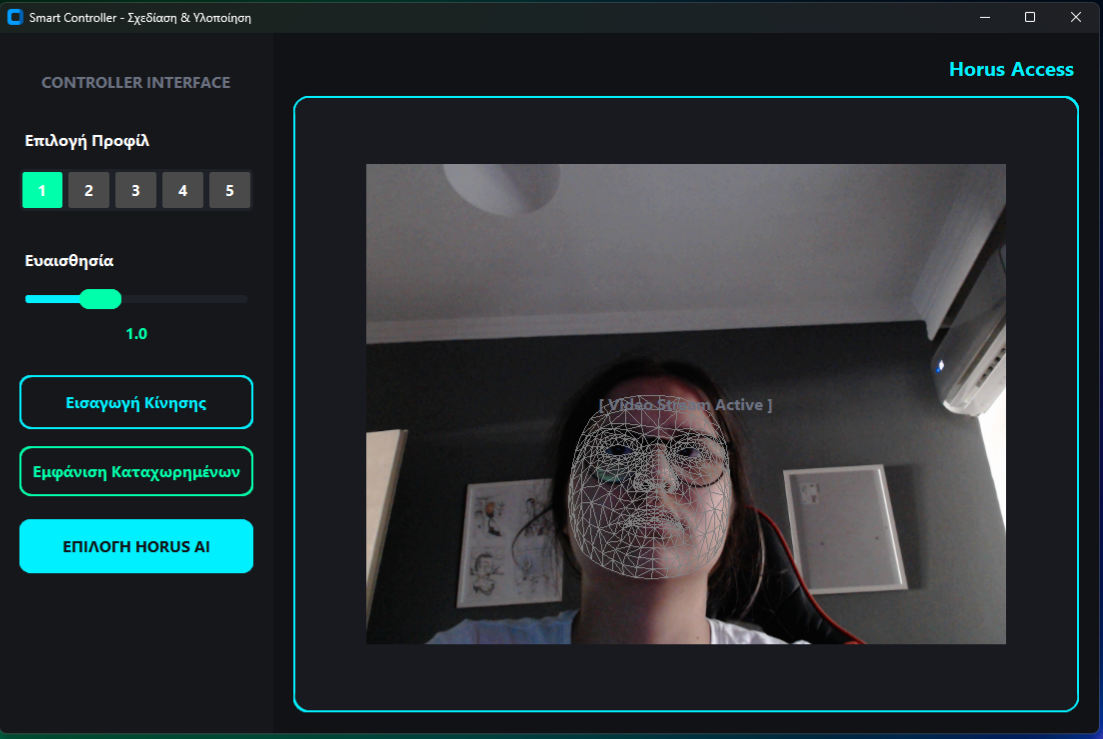
\includegraphics[width=0.85\textwidth]{userInterface.png}
    \caption{Το κεντρικό περιβάλλον χρήστη (UI) του HorusAccess.}
    \label{fig:main_ui}
\end{figure}

\textbf{2. Ανίχνευση Προσώπου και Υπολογισμός Κίνησης Κεφαλιού}\\
Κάθε καρέ που λαμβάνεται από την κάμερα αναστρέφεται οριζόντια (\textlatin{horizontal flip}) και μετατρέπεται σε \textlatin{RGB} προκειμένου να υποβληθεί σε επεξεργασία από το \textlatin{MediaPipe Face Mesh}. Το σύστημα υπολογίζει τις γωνίες κλίσης του κεφαλιού (\textlatin{Roll} για οριζόντια κίνηση και \textlatin{Pitch} για κατακόρυφη) εφαρμόζοντας ζώνες ανοχής (\textlatin{deadzones}), ώστε να εξαλειφθούν οι ακούσιες μικροκινήσεις:

\begin{verbatim}
# Υπολογισμός Γωνίας Κλίσης Κεφαλιού (Roll - Δεξιά/Αριστερά)
roll_tilt = right_face.y - left_face.y

# Υπολογισμός Πάνω/Κάτω (Pitch)
face_center_y = (top_face.y + bottom_face.y) / 2.0
pitch_tilt = nose.y - face_center_y
\end{verbatim}

Αμέσως με την εκκίνηση, ενεργοποιείται ο μηχανισμός \textlatin{head-tracking} για τον έλεγχο του δείκτη. Παράλληλα, ενσωματώνεται μηχανισμός ασφαλείας προσωρινής αναστολής (\textlatin{Mouse Override}), ο οποίος ανιχνεύει αν ο χρήστης κινήσει το φυσικό ποντίκι, αποτρέποντας την αυτόματη επαναφορά του δείκτη για καθορισμένο χρονικό διάστημα (\texttt{MOUSE\_OVERRIDE\_SECONDS = 3.0})[cite: 1], επιτρέποντας σε έναν φροντιστή να λάβει τον έλεγχο εφόσον απαιτηθεί. Για τη μεγιστοποίηση της προσβασιμότητας, η διεπαφή διαθέτει κουμπιά μεγάλου μεγέθους (\texttt{height=50--55px}) για εύκολη στόχευση, καθώς και λειτουργία μαγνητικής προσκόλλησης (\textlatin{magnetic cursor}) μέσω του \texttt{SnapCursorMixin}.

\textbf{3. Διαχείριση Προφίλ και Εισαγωγή Κινήσεων}\\
Το σύστημα υποστηρίζει πολλαπλά προφίλ χρήστη (1 έως 5)[cite: 1]. Μέσω του \texttt{profile\_selector} αποτρέπεται η ανάγκη επαναρύθμισης των επιλογών σε κάθε αλλαγή παιχνιδιού. Μέσω του παραθύρου \texttt{ProfileReviewWindow}, ο χρήστης μπορεί να επισκοπεί ή να διαγράφει τις αποθηκευμένες αντιστοιχίσεις του εκάστοτε προφίλ (Σχήμα~\ref{fig:profile_mgmt})[cite: 1].

\begin{figure}[H]
    \centering
    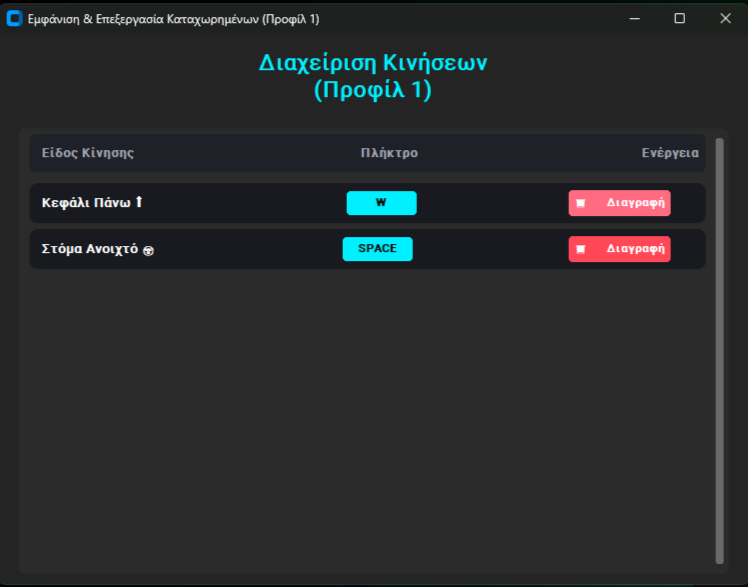
\includegraphics[width=0.85\textwidth]{diaxeirishprofile.png}
    \caption{Διαχείριση και επισκόπηση προφίλ.}
    \label{fig:profile_mgmt}
\end{figure}

Η διαδικασία χειροκίνητης εισαγωγής κίνησης ενεργοποιείται από το κουμπί \texttt{btn\_add\_motion} μέσω της κλάσης \texttt{MotionInputWindow}[cite: 1] και ολοκληρώνεται σε δύο διαδοχικά βήματα: αρχικά πραγματοποιείται η επιλογή της επιθυμητής κίνησης προσώπου και στη συνέχεια, μέσω ενός εικονικού πληκτρολογίου στα δεξιά, ο χρήστης επιλέγει την αντιστοίχιση με το αντίστοιχο πλήκτρο, αποθηκεύοντας τη σύνδεση στο ενεργό προφίλ (Σχήμα~\ref{fig:key_mapping}).
\begin{figure}[H]
    \centering
    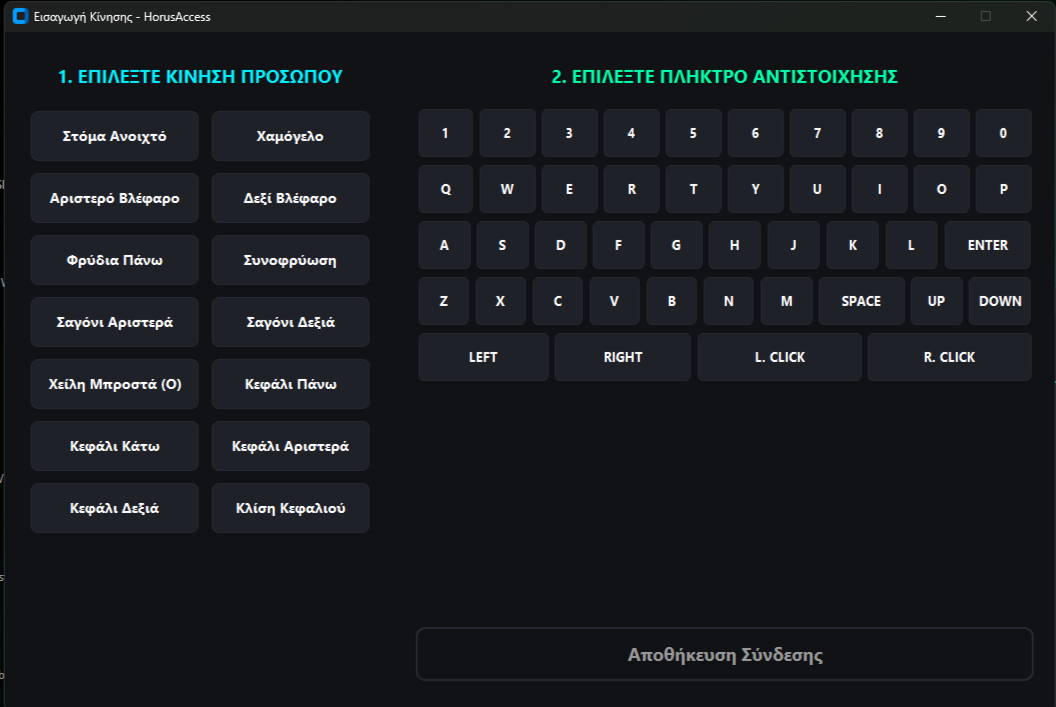
\includegraphics[width=0.85\textwidth]{eisagwghKinhshs.png}
    \caption{Εισαγωγή κίνησης και αντιστοίχιση πλήκτρου.}
    \label{fig:key_mapping}
\end{figure}

\textbf{4. Αυτόνομη Επιλογή Παιχνιδιών και Horus AI}\\
Το σημαντικότερο δομικό στοιχείο της εφαρμογής αποτελεί η ενότητα \textbf{Horus AI} (που καλείται μέσω του κουμπιού \texttt{btn\_auto\_select} και της κλάσης \texttt{AutonomousGameSelectorWindow}[cite: 1]), η οποία αυτοματοποιεί τη διαδικασία παραμετροποίησης των κινήσεων, μειώνοντας τον απαιτούμενο χρόνο και κόπο. Το \textlatin{Horus AI} ανιχνεύει τα εγκατεστημένα παιχνίδια του υπολογιστή και τα προβάλλει σε μορφή δυναμικού πλέγματος καρτών (\textlatin{Scrollable Grid})[cite: 1] εμφανίζοντας την εικόνα εξωφύλλου, τον τίτλο και την πλατφόρμα εγκατάστασής τους (Σχήμα~\ref{fig:game_selector}). Η ανίχνευση εκτελείται σε ξεχωριστό \textlatin{worker thread} ώστε να μη «παγώνει» το \textlatin{UI event loop}.

\begin{figure}[H]
    \centering
    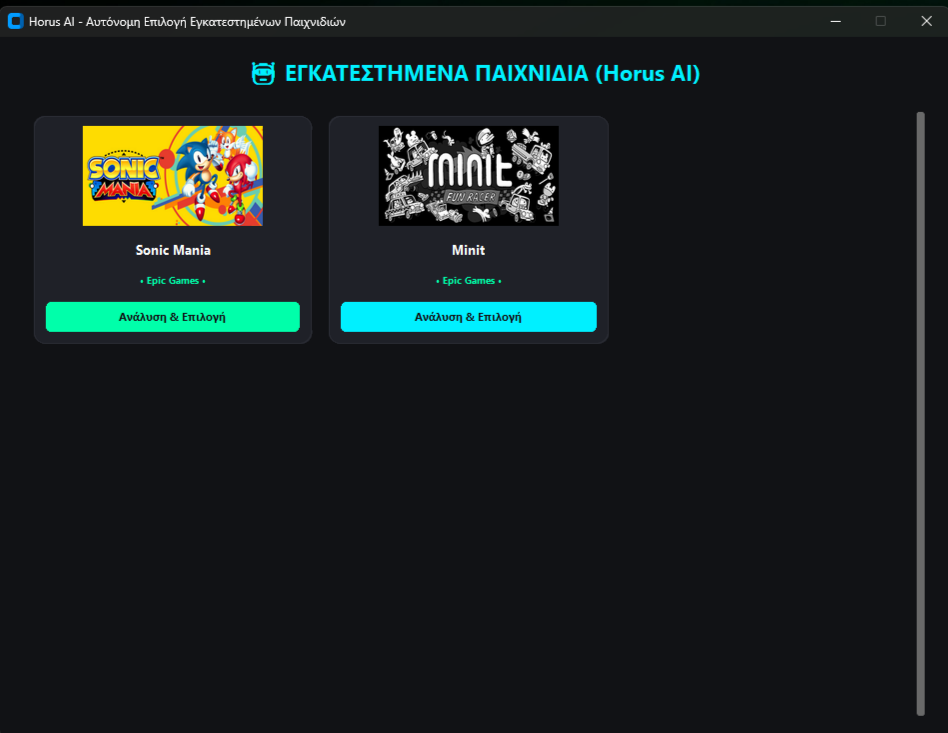
\includegraphics[width=0.85\textwidth]{horusAi.png}
    \caption{Επιλογή εγκατεστημένου παιχνιδιού στο Horus AI.}
    \label{fig:game_selector}
\end{figure}

Όταν ο χρήστης επιλέξει έναν τίτλο, το σύστημα επικοινωνεί αυτόματα με το τοπικό \textlatin{Ollama LLM} (μοντέλο \textlatin{llama3.2})[cite: 1] για την παραγωγή των βέλτιστων αντιστοιχίσεων. Το σύστημα ενημερώνει τον χρήστη μέσω σχετικού αναδυόμενου παραθύρου επιβεβαίωσης και, με την αποδοχή του («OK / Αποδοχή»), οι προτεινόμενες αντιστοιχίσεις επικυρώνονται και αποθηκεύονται άμεσα στο επιλεγμένο προφίλ (Σχήμα~\ref{fig:ai_suggestion}).

\begin{figure}[H]
    \centering
    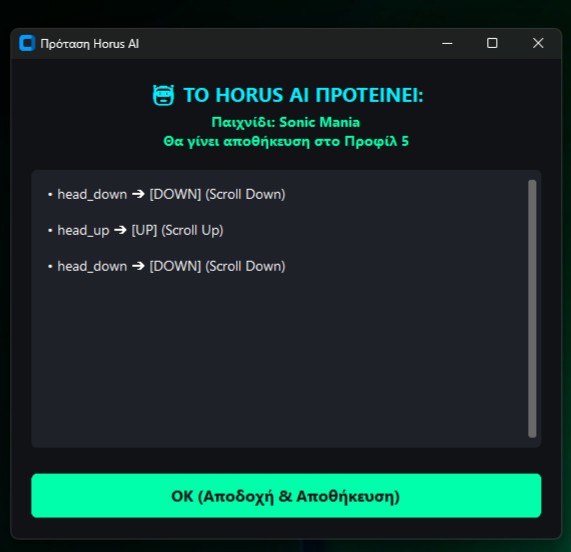
\includegraphics[width=0.85\textwidth]{Aisuggestion.png}
    \caption{Μήνυμα πρότασης αλγορίθμου Horus AI.}
    \label{fig:ai_suggestion}
\end{figure}

Συνοψίζοντας, ο σχεδιασμός και η υλοποίηση του \textlatin{HorusAccess} πραγματοποιήθηκαν με πρωταρχικό γνώμονα την ευχρηστία, την προσβασιμότητα και την υψηλή αισθητική, παραπέμποντας σε σύγχρονο λογισμικό βιντεοπαιχνιδιών (\textlatin{gaming software}) και ενισχύοντας ουσιαστικά το αίσθημα της συμπερίληψης και της ισότιμης συμμετοχής των ατόμων με αναπηρία στον ψηφιακό κόσμο.

\subsection{Διαχείριση Δεδομένων και Αποθήκευση}

Για την λειτουργία του συστήματος \textlatin{HorusAccess} και τη διασφάλιση της μόνιμης αποθήκευσης των εξατομικευμένων ρυθμίσεων, των προφίλ χρηστών και των αντιστοιχίσεων κινήσεων, απαιτείται ένας αξιόπιστος και ελαφρύς μηχανισμός διαχείρισης δεδομένων. Η αρχιτεκτονική αποθήκευσης του λογισμικού σχεδιάστηκε με γνώμονα την αυτονομία, την ταχύτητα αποκρίσεων και την αποφυγή εξωτερικών εξαρτήσεων από περίπλοκους διακομιστές βάσεων δεδομένων, καθιστώντας την εφαρμογή ανεξάρτητη από το περιβάλλον εκτέλεσης.

\subsection{Σχήμα Βάσης Δεδομένων SQLite}

Η επιμέρους διαχείριση της επιμονής των δεδομένων (\textlatin{persistence layer}) υλοποιείται μέσω του ενσωματωμένου συστήματος διαχείρισης σχεσιακών βάσεων δεδομένων \textlatin{SQLite}, αξιοποιώντας αποκλειστικά τοπικά αρχεία εντός του αρχείου \texttt{database/db\_manager.py}. Κατά την αρχικοποίηση της κλάσης \texttt{DBManager}, το σχήμα της βάσης οργανώνεται γύρω από τρεις βασικούς πίνακες που αποθηκεύουν τα προφίλ χρηστών, τις τρέχουσες τιμές ευαισθησίας, καθώς και το δυναμικό μητρώο αντιστοιχίσεων:

\begin{verbatim}
def _create_tables(self):
    """Δημιουργεί τους πίνακες με ενσωματωμένο το threshold."""
    with self._connection() as conn:
        cursor = conn.cursor()
        
        # Πίνακας Προφίλ
        cursor.execute('''
            CREATE TABLE IF NOT EXISTS profiles (
                id INTEGER PRIMARY KEY CHECK (id >= 1 AND id <= 5),
                name TEXT NOT NULL,
                sensitivity REAL DEFAULT 1.0
            )
        ''')
        
        # Πίνακας Αντιστοιχίσεων (Ενημερωμένος)
        cursor.execute('''
            CREATE TABLE IF NOT EXISTS mappings (
                id INTEGER PRIMARY KEY AUTOINCREMENT,
                profile_id INTEGER,
                action TEXT NOT NULL,
                mapped_key TEXT NOT NULL,
                threshold REAL DEFAULT 0.05,
                FOREIGN KEY (profile_id) REFERENCES profiles(id),
                UNIQUE(profile_id, action)
            )
        ''')

        # Πίνακας Ρυθμίσεων (key/value) - π.χ. τελευταίο ενεργό προφίλ
        cursor.execute('''
            CREATE TABLE IF NOT EXISTS settings (
                key TEXT PRIMARY KEY,
                value TEXT
            )
        ''')
\end{verbatim}

\subsubsection{Συστήματα Προφίλ και Διατήρηση Δεδομένων}
Προκειμένου να καλυφθούν οι διαφορετικές ανάγκες των χρηστών αλλά και η εναλλαγή ανάμεσα σε πολλαπλά ψηφιακά παιχνίδια ή εφαρμογές γραφείου, το \textlatin{HorusAccess} υποστηρίζει τη διαχείριση πολλαπλών διακριτών προφίλ (αριθμημένων από 1 έως 5). Κάθε προφίλ λειτουργεί ως ένα αυτόνομο περιβάλλον ελέγχου, αποθηκεύοντας τις αποκλειστικές αντιστοιχίσεις κινήσεων, τα προσαρμοσμένα όρια ενεργοποίησης (\textlatin{thresholds}), καθώς και τον τίτλο της εφαρμογής.

Η ασφαλής διαχείριση των συναλλαγών επιτυγχάνεται μέσω ενός \textlatin{context manager} σύνδεσης που διαχειρίζεται αυτόματα τις διαδικασίες \textlatin{commit} και \textlatin{rollback} σε περίπτωση σφάλματος. Παράλληλα, η μέθοδος \texttt{save\_mapping} διασφαλίζει την αποφυγή διπλοεγγραφών ανά προφίλ και κίνηση, αξιοποιώντας την κανονικοποίηση πλήκτρων και ενεργειών:

\begin{verbatim}
def save_mapping(self, profile_id: int, action: str, mapped_key: str,
                   threshold=None, default_threshold=0.05):
    """Αποθηκεύει τη νέα κίνηση και το όριό της."""
    mapped_key = canonical_key(mapped_key)
    if not mapped_key:
        raise ValueError("Το mapped_key δεν μπορεί να είναι κενό.")

    canonical_action = canonical_motion(action)
    if canonical_action is not None:
        action = canonical_action

    with self._connection() as conn:
        cursor = conn.cursor()
        cursor.execute('''
            INSERT INTO mappings (profile_id, action, mapped_key, threshold)
            VALUES (?, ?, ?, COALESCE(?, ?))
            ON CONFLICT(profile_id, action) DO UPDATE SET
                mapped_key = excluded.mapped_key,
                threshold = COALESCE(?, mappings.threshold, ?)
        ''', (profile_id, action, mapped_key, threshold,
              default_threshold, threshold, default_threshold))
\end{verbatim}

Επιπλέον, η κλάση ενσωματώνει εξειδικευμένους μηχανισμούς αυτόματης αναβάθμισης (\textlatin{migrations}, όπως τα \texttt{migrate\_legacy\_thresholds}, \texttt{migrate\_legacy\_key\_aliases} και \texttt{migrate\_legacy\_action\_aliases}), οι οποίοι εξασφαλίζουν την απρόσκοπτη μεταφορά παλαιότερων δομών στη νέα κανονικοποιημένη μορφή χωρίς να χάνονται οι εξατομικευμένες ρυθμίσεις του χρήστη.

\textbf{1. Κίνηση Δείκτη Ποντικιού (\textlatin{Pointer Movement})}\\
Η κίνηση του δείκτη βασίζεται στην ανάλυση των χαρακτηριστικών του προσώπου ανά καρέ:
\begin{enumerate}
    \item Το καρέ αναστρέφεται οριζόντια, ώστε ο χρήστης να κινεί το κεφάλι του φυσικά, σαν να κοιτάζει την οθόνη.
    \item Η γωνία κλίσης \textlatin{Roll} (\texttt{right\_face.y - left\_face.y}) οδηγεί την οριζόντια κίνηση, ενώ η κλίση \textlatin{Pitch} (\texttt{nose.y - face\_center\_y}) οδηγεί την κατακόρυφη κίνηση.
    \item Εφαρμόζονται ζώνες ανοχής (\textlatin{deadzones}, 0.025 για το \textlatin{roll} και 0.005 για το \textlatin{pitch}) για την καταστολή του θορύβου, ενώ ο ρυθμιστής ευαισθησίας (\textlatin{sensitivity slider}) προσαρμόζει την εναπομείνασα κίνηση.
    \item Ο εικονικός δρομέας περιορίζεται στα όρια της οθόνης και περνάει μέσα από τον μηχανισμό \texttt{SnapCursorMixin.\_snap\_cursor()}.
    \item Η συνάρτηση \texttt{input\_backend.mouse\_move()} επιλέγει τη διαδρομή ανάλογα με το λειτουργικό σύστημα:
    \begin{itemize}
        \item Στο \textlatin{sway}: χρήση \textlatin{IPC} για ρύθμιση της θέσης του δείκτη και εστίαση του παραθύρου κάτω από αυτόν.
        \item Σε \textlatin{Linux} με \textlatin{pynput}: χρήση του \texttt{mouse.Controller.position}.
        \item Διαφορετικά: χρήση \textlatin{pyautogui / pydirectinput moveTo()}.
    \end{itemize}
    \item Κάθε θέση που εγχέεται καταγράφεται ως \textlatin{warp}, ώστε η επόμενη μέτρηση του φυσικού ποντικιού να μπορεί να διακρίνει τη συνθετική κίνηση από μια πραγματική κίνηση χεριού.
\end{enumerate}


\textbf{2. Παράκαμψη Φυσικού Ποντικιού (\textlatin{Physical-Mouse Override})}\\
Η συνάρτηση \texttt{input\_backend.mouse\_activity\_count()} αυξάνεται όταν ο πραγματικός δείκτης κινείται χωρίς αντίστοιχη καταγραφή \textlatin{warp}. Όταν ο μετρητής αλλάξει, η εφαρμογή θέτει σε προσωρινή παύση τα \textlatin{warps} που βασίζονται στο κεφάλι για χρονικό διάστημα \texttt{MOUSE\_OVERRIDE\_SECONDS} (3 δευτερόλεπτα) και συνεχίζει να συγχρονίζει τον εικονικό δρομέα με τον πραγματικό δείκτη. Η λειτουργία αυτή υποστηρίζεται σε \textlatin{Windows, X11} και \textlatin{macOS}, ενώ στο \textlatin{sway} ο έλεγχος βασίζεται στον κατοπτρικό δείκτη του \textlatin{XWayland}, καλύπτοντας το \textlatin{UI} της εφαρμογής και τα παιχνίδια \textlatin{XWayland}. Όταν η ιχνηλάτηση απενεργοποιείται, ο εικονικός δρομέας συγχρονίζεται εκ νέου και ο μετρητής δραστηριότητας ανανεώνεται, ώστε η επανενεργοποίηση να μην προκαλεί άμεση ενεργοποίηση της παράκαμψης.

\textbf{3. Διαχείριση και Αποστολή Χειρονομιών (\textlatin{Gesture Dispatch})}\\
\begin{enumerate}
    \item Η συνάρτηση \texttt{compute\_facial\_metrics(landmarks)} επιστρέφει τις τιμές των μετρικών του προσώπου.
    \item Το \texttt{HeadPoseTracker.update(landmarks)} προσθέτει τις καλιμπραρισμένες μετρικές κεφαλιού. Η πρώτη ουδέτερη στάση καταγράφεται αυτόματα, ενώ η επιλογή «Επαναφορά Κέντρου» την επαναφέρει.
    \item Για κάθε ενεργή αντιστοίχιση, η συνάρτηση \texttt{is\_gesture\_active(action, value, threshold)} εφαρμόζει την κατεύθυνση της χειρονομίας (τιμή > \textlatin{threshold} για τις περισσότερες χειρονομίες, τιμή < \textlatin{threshold} για τα βλεφαρίσματα, τις συνοφρυώσεις, το σαγόνι και το στράβωμα μυτητής).
    \item Ο αποστολέας δομεί ένα επιθυμητό σύνολο πλήκτρων και το συγκρίνει με τα πατημένα πλήκτρα (\texttt{pressed\_keys}):
    \begin{itemize}
        \item Τα πλήκτρα που υπάρχουν μόνο στο επιθυμητό σύνολο πιέζονται.
        \item Τα πλήκτρα που υπάρχουν μόνο στο σύνολο πίεσης απελευθερώνονται.
    \end{itemize}
    \item Εάν δεν ανιχνευθεί πρόσωπο, εκτελείται η συνάρτηση \texttt{\_release\_all\_keys()}, αποτρέποντας το κόλλημα κάποιο πλήκτρου όταν χάνεται η ιχνηλάτηση.
\end{enumerate}
Η αντιστοίχιση του ίδιου πλήκτρου από δύο κινήσεις είναι ασφαλής: το πλήκτρο παραμένει πατημένο έως ότου η τελευταία κίνηση το απελευθερώσει.

\textbf{4. Βελτιστοποίηση Προβολής (\textlatin{Preview Optimization})}\\
Το πλαίσιο \textlatin{RGB} αντιγράφεται σε ένα επαναχρησιμοποιήσιμο αντικείμενο \texttt{ImageTk.PhotoImage}, με το πλέγμα προσώπου να σχεδιάζεται μόνο όταν η μεταβλητή \texttt{SHOW\_FACE\_MESH} είναι \textlatin{True}. Η επαναχρησιμοποίηση της εικόνας αποτρέπει τη συνεχή δέσμευση μνήμης ανά καρέ, ενώ η παράμετρος \texttt{SHOW\_FACE\_MESH} διαβάζεται μία φορά κατά την εκκίνηση.
\subsection{Περιορισμοί Συστήματος και Ειδικές Περιπτώσεις}

Η υλοποίηση ενός συστήματος ελέγχου βασισμένου σε κάμερα και συνθετική είσοδο (\textlatin{synthetic input}) σε πολλαπλά λειτουργικά συστήματα συνοδεύεται από τεχνικούς περιορισμούς, κυρίως λόγω των αρχιτεκτονικών διαφορών μεταξύ των παραδοσιακών διακομιστών παραθύρων (\textlatin{X11, Windows, macOS}) και των σύγχρονων περιβαλλόντων ασφαλείας, όπως το \textlatin{Wayland}.

\subsubsection{Περιορισμοί Συνθετικής Εισόδου ανά Λειτουργικό}

Ο μηχανισμός διαχείρισης εισόδου του \textlatin{HorusAccess} (\texttt{core/input\_backend.py}) προσαρμόζεται δυναμικά ανάλογα με το λειτουργικό σύστημα:
\begin{itemize}
    \item \textbf{Windows:} Η χρήση των βιβλιοθηκών \textlatin{pydirectinput} και \textlatin{pyautogui} διασφαλίζει ότι η έγχυση κωδικών σαρωτή (\textlatin{Scan Codes}) φτάνει επιτυχώς σε παιχνίδια βασισμένα στο \textlatin{DirectX}.
    \item \textbf{Linux (X11):} Προτιμάται η βιβλιοθήκη \textlatin{pynput} για υψηλή αξιοπιστία στην αποστολή συμβάντων πληκτρολογίου και ποντικιού, με \textlatin{fallback} μηχανισμό σε \textlatin{pyautogui/XTest}.
    \item \textbf{macOS:} Απαιτείται η ρητή παραχώρηση δικαιωμάτων προσβασιμότητας (\textlatin{Accessibility Permissions}) στο τερματικό από το οποίο εκτελείται η εφαρμογή, προκειμένου να επιτραπεί η έγχυση γεγονότων μέσω του \textlatin{Quartz} (\textlatin{pyautogui}).
\end{itemize}

\subsubsection{Συμπεριφορά σε Wayland / XWayland}

Στα περιβάλλοντα \textlatin{Linux} με συνθέτη παραθύρων \textlatin{Wayland} (και ειδικότερα στο \textlatin{sway}), η ασφάλεια του πρωτοκόλλου απαγορεύει στις εφαρμογές να παρακολουθούν ή να ελέγχουν αυθαίρετα τον κέρσορα. Για την αντιμετώπιση αυτού του περιορισμού, το σύστημα ενεργοποιεί την ειδική διαδρομή \textlatin{sway IPC} εφόσον εντοπιστούν οι μεταβλητές περιβάλλοντος \textlatin{WAYLAND\_DISPLAY} και \textlatin{SWAYSOCK}:
\begin{itemize}
    \item \textbf{Έγχυση Κέρσορα και Εστίαση:} Ο δείκτη του συνθέτη μετακινείται μέσω της εντολής \textlatin{seat - cursor set}, ενώ το παράθυρο κάτω από τον δείκτη λαμβάνει αυτόματα εστίαση (\textlatin{focus}), εξομοιωμένοι τη λειτουργία \textlatin{focus\_follows\_mouse}. Αυτό επιτρέπει στα στοιχεία ελέγχου της εφαρμογής να αντιλαμβάνονται τα γεγονότα \textlatin{hover} και \textlatin{clicks}.
    \item \textbf{Περιορισμοί Εγγενών Εφαρμογών Wayland:} Επειδή το \textlatin{Wayland} αγνοεί τα \textlatin{XTest warps}, η έγχυση πληκτρολογίου και κλικ ενδέχεται να αγνοηθεί από καθαρόαιμες, εγγενείς εφαρμογές \textlatin{Wayland}. Αντίθετα, η παράκαμψη φυσικού ποντικιού (\textlatin{physical-mouse override}) λειτουργεί κανονικά πάνω από το \textlatin{UI} της εφαρμογής και τα παιχνίδια \textlatin{XWayland}, αξιοποιώντας την κατοπτρική απεικόνιση του δείκτη.
\end{itemize}

\subsection{Αντιμετώπιση Προκλήσεων και Σφάλματα Κώδικα (Bug Tracking)}

Κατά την ανάπτυξη και τον ενδελεχή έλεγχο κώδικα (\textlatin{code review}) του συστήματος \textlatin{HorusAccess}, εντοπίστηκαν και καταγράφηκαν συνολικά 36 τεχνικά ζητήματα και σφάλματα (\textlatin{bugs}) που αφορούσαν διαφορετικά υποσυστήματα της εφαρμογής (εντοπισμός χειρονομιών, γραφικό περιβάλλον, βάση δεδομένων, ενσωμάτωση LLM, ανίχνευση παιχνιδιών και υποσύστημα εισόδου). Η επίλυσή τους οργανώθηκε και υλοποιήθηκε σε τρεις διακριτές φάσεις (\textlatin{Batches 1--3}), διασφαλίζοντας την ακεραιότητα, τη σταθερότητα και την υψηλή απόκριση του λογισμικού.

\subsubsection{Κατηγοριοποίηση και Σοβαρότητα Σφαλμάτων}
Τα ζητήματα ταξινομήθηκαν βάσει της σοβαρότητάς τους σε τέσσερα επίπεδα:
\begin{itemize}
    \item \textbf{S1 (Critical):} Κρίσιμα σφάλματα που απέτρεπαν τη λειτουργία βασικών χαρακτηριστικών (π.χ. αδυναμία ενεργοποίησης πλήκτρων από κινήσεις κεφαλιού, αναστροφή αξόνων).
    \item \textbf{S2 (High):} Σοβαρά σφάλματα που προκαλούσαν εξαιρέσεις (\textlatin{exceptions}), παγώματα του UI ή εσφαλμένη συμπεριφορά δεδομένων.
    \item \textbf{S3 (Medium):} Προβλήματα μεσαίας προτεραιότητας σχετικά με τη δομή της βάσης δεδομένων, τη συμβατότητα και την ευστάθεια των ανιχνευτών.
    \item \textbf{S4 (Low):} Ζητήματα χαμηλής προτεραιότητας που αφορούσαν αχρησιμοποίητο κώδικα (\textlatin{dead code}) ή βελτιστοποιήσεις.
\end{itemize}

\subsubsection{Σημαντικότερες Κατηγορίες Σφαλμάτων και Λύσεις}

\begin{enumerate}
    \item \textbf{Υποσύστημα Χειρονομιών (\textlatin{Gestures}):}
    \begin{itemize}
        \item \emph{Πρόβλημα:} Οι κινήσεις του κεφαλιού (\textlatin{head\_up, head\_down, head\_left, head\_right}) δεν διέθεταν αντίστοιχες μετρικές στο \textlatin{MediaPipe}, με αποτέλεσμα να αγνοούνται πλήρως από τον αποστολέα γεγονότων. Παράλληλα, το προεπιλεγμένο κατώφλι (\textlatin{threshold}) του $0.05$ προκαλούσε τη μόνιμη ενεργοποίηση ορισμένων χειρονομιών και την αδυναμία ενεργοποίησης άλλων.
        \item \emph{Λύση:} Ενσωματώθηκε σύστημα καλιμπραρίσματος ουδέτερης στάσης κεφαλιού (\textlatin{HeadPoseTracker}) με δυναμικές αποκλίσεις, ορίστηκαν ξεχωριστά κατώφλια ανά χειρονομία και εφαρμόστηκε αυτόματη απελευθέρωση πλήκτρων σε περίπτωση απώλειας ανίχνευσης προσώπου (\textlatin{face loss}).
    \end{itemize}

    \item \textbf{Διαχείριση Βάσης Δεδομένων και Αποθήκευση (\textlatin{Database}):}
    \begin{itemize}
        \item \emph{Πρόβλημα:} Η χρήση \textlatin{INSERT OR REPLACE} σε συνδυασμό με \textlatin{AUTOINCREMENT} άλλαζε τα αναγνωριστικά (\textlatin{row IDs}) των αντιστοιχίσεων σε κάθε αποθήκευση, ενώ οι συνδέσεις της \textlatin{SQLite} παρέμειναν ανοιχτές προκαλώντας διαρροές πόρων.
        \item \emph{Λύση:} Υιοθετήθηκε η δομή \textlatin{UPSERT} (\textlatin{ON CONFLICT ... DO UPDATE}) για τη διατήρηση των \textlatin{IDs} και δημιουργήθηκε διαχειριστής συμφραζομένων (\textlatin{context manager}) που διασφαλίζει το κλείσιμο των συνδέσεων και την ορθή εκτέλεση \textlatin{commit/rollback}.
    \end{itemize}

    \item \textbf{Απόκριση Διεπαφής και Ενσωμάτωση LLM (\textlatin{GUI \& Ollama}):}
    \begin{itemize}
        \item \emph{Πρόβλημα:} Η σύγχρονη κλήση του τοπικού μοντέλου \textlatin{Ollama} καθώς και η σάρωση αρχείων και λήψη εικόνων από το \textlatin{CDN} εκτελούνταν απευθείας στο κύριο νήμα (\textlatin{Tk main thread}), παγώνοντας προσωρινά ολόκληρη τη γραφική διεπαφή.
        \item \emph{Λύση:} Οι βαριές λειτουργίες μεταφέρθηκαν σε αυτόνομα υπο-νήματα (\textlatin{worker threads}), αξιοποιώντας ουρές ασφαλούς επικοινωνίας (\textlatin{queue.Queue}) και την εντολή \textlatin{after()} για την ενημέρωση του UI χωρίς καθυστερήσεις.
    \end{itemize}

    \item \textbf{Ανίχνευση Παιχνιδιών και Backends Εισόδου:}
    \begin{itemize}
        \item \emph{Πρόβλημα:} Οι διαδρομές με κενά στα αρχεία \textlatin{.desktop} έσπαγαν την ανάλυση των εντολών \textlatin{Exec=}, ενώ τα ονόματα πλήκτρων παρουσίαζαν ασυνέπειες μεταξύ των διαφορετικών λειτουργικών συστημάτων (\textlatin{Windows, Linux, macOS}).
        \item \emph{Λύση:} Εφαρμόστηκε ασφαλής ανάλυση με τη βιβλιοθήκη \textlatin{shlex}, καθιερώθηκε εσωτερική κανονικοποίηση ονομάτων πλήκτρων (\textlatin{canonical key names}) και προστέθηκαν μηχανισμοί απομόνωσης σφαλμάτων ανά ανιχνευτή (\textlatin{per-detector error isolation}), ώστε μια αποτυχημένη σάρωση να μην εμποδίζει τις υπόλοιπες πλατφόρμες.
    \end{itemize}
\end{enumerate}

Χάρη σε αυτές τις διορθώσεις και την προσθήκη εκτεταμένου αυτοματοποιημένου ελέγχου μονάδας (\textlatin{unittest suite} με πάνω από 64 επιτυχημένες δοκιμές χωρίς εξωτερικές εξαρτήσεις), το σύστημα \textlatin{HorusAccess} απέκτησε υψηλή ανθεκτικότητα, αποτρέποντας ακούσιες εμπλοκές πλήκτρων και διασφαλίζοντας ομαλή εμπειρία χρήσης για άτομα με αναπηρία.


\subsection{Σύνοψη Κεφαλαίου}

\begin{itemize}
    \item \textbf{Συνοπτική Επισκόπηση:} Το κεφάλαιο παρουσιάζει την τεχνική υλοποίηση του συστήματος \textlatin{HorusAccess}, το οποίο επιτρέπει τον έλεγχο υπολογιστών και ψηφιακών παιχνιδιών μέσω κινήσεων κεφαλιού και εκφράσεων προσώπου, διαθέτοντας αυτονομία και δυνατότητες τοπικής τεχνητής νοημοσύνης.
    \item \textbf{Πυρήνας και Υποσυστήματα (\texttt{core/}):} Η ανίχνευση κινήσεων υλοποιείται μέσω του \textlatin{MediaPipe Face Mesh} για τον υπολογισμό μετρικών προσώπου και καλιμπράρισμα ουδέτερης στάσης κεφαλιού (\texttt{HeadPoseTracker}), ενώ η διαχείριση εισόδου (\texttt{input\_backend.py}) υποστηρίζει πολλαπλά λειτουργικά συστήματα με μηχανισμό προσωρινής παράκαμψης φυσικού ποντικιού (\textlatin{Mouse Override}).
    \item \textbf{Αυτόματος Εντοπισμός και AI (\texttt{game\_detector.py} \& \texttt{ai\_mappings.py}):} Το σύστημα σαρώνει εγκατεστημένους τίτλους από δημοφιλείς πλατφόρμες (\textlatin{Steam, Epic Games, GOG}) και συνεργάζεται με τοπικά γλωσσικά μοντέλα μέσω του \textlatin{Ollama} (μοντέλο \textlatin{llama3.2}) για την αυτόματη παραγωγή και επικύρωση διατάξεων ελέγχου (\textlatin{Key Mappings}) ανάλογα με το είδος του παιχνιδιού.
    \item \textbf{Διαχείριση Δεδομένων (\texttt{database/}):} Η επιμονή των δεδομένων βασίζεται σε τοπική βάση δεδομένων \textlatin{SQLite} (\texttt{db\_manager.py}) για προφίλ χρηστών, τιμές ευαισθησίας και ρυθμίσεις, αξιοποιώντας διαχειριστές συμφραζομένων (\textlatin{context managers}), δομές \textlatin{UPSERT} και αυτόματες αναβαθμίσεις σχήματος (\textlatin{migrations}).
    \item \textbf{Γραφική Διεπαφή Χρήστη (\texttt{gui/main.py}):} Κατασκευασμένο με τη βιβλιοθήκη \textlatin{CustomTkinter} σε σκούρο θέμα («\textlatin{Modern Stealth}»), το γραφικό περιβάλλον ενσωματώνει ζωντανή προβολή βίντεο κάμερας, επιλογή προφίλ, ρυθμιστές ευαισθησίας, εικονικό πληκτρολόγιο και λειτουργία μαγνητικού δρομέα (\texttt{SnapCursorMixin}).
    \item \textbf{Ασύγχρονη Εκτέλεση και Απόδοση:} Οι βαριές διεργασίες (σάρωση παιχνιδιών, λήψη εικόνων \textlatin{CDN}, κλήσεις \textlatin{LLM}) εκτελούνται σε ανεξάρτητα υπονήματα (\textlatin{worker threads}) επικοινωνώντας με το κύριο νήμα μέσω ασφαλών ουρών (\texttt{queue.Queue}), αποτρέποντας τα παγώματα του \textlatin{UI}.
    \item \textbf{Περιορισμοί και Bug Tracking:} Αναλύονται οι περιορισμοί ασφαλείας των περιβαλλόντων \textlatin{Wayland} (μέσω της ειδικής διαδρομής \textlatin{Sway IPC}), καθώς και η συστηματική επίλυση 36 τεχνικών σφαλμάτων και βελτιστοποιήσεων που επαληθεύτηκαν με εκτεταμένη σουίτα αυτοματοποιημένων ελέγχων (\textlatin{unittest suite}).
\end{itemize}

\clearpage
\section{Αξιολόγηση Εφαρμογής}

\subsection{Εισαγωγή}
Στο παρόν κεφάλαιο παρουσιάζεται η συστηματική αξιολόγηση της αναπτυχθείσας εφαρμογής ως προς την ευχρηστία και τη συνολική εμπειρία χρήστη. Αρχικά, αναλύονται οι αντικειμενικοί στόχοι και η μεθοδολογία της πειραματικής διαδικασίας, ενώ στη συνέχεια παρατίθενται και σχολιάζονται τα ποσοτικά και ποιοτικά αποτελέσματα που προέκυψαν.

\subsection{Στόχοι Αξιολόγησης}

Η αξιολόγηση αποσκοπεί στη διερεύνηση της λειτουργικότητας, της αποδοτικότητας και της ευχρηστίας του συστήματος αλληλεπίδρασης για άτομα με κινητική αναπηρία. Εξετάζεται κατά πόσο η παρούσα υλοποίηση ανταποκρίνεται στις προκαθορισμένες τεχνικές απαιτήσεις, ενώ παράλληλα επιδιώκεται ο εντοπισμός ενδεχόμενων περιορισμών κατά την πραγματική χρήση.

Ειδικότερα, οι βασικοί άξονες της αξιολόγησης εστιάζουν στην αποτίμηση του μηχανισμού ελέγχου (ακρίβεια και ομαλότητα στην κίνηση του κέρσορα μέσω της κεφαλής, καθώς και αποτελεσματικότητα των εκφράσεων του προσώπου για την εκτέλεση ενεργειών), στη διερεύνηση της ευχρηστίας κατά τον ανέπαφο χειρισμό χωρίς τη χρήση των άνω άκρων, και στην ολική αποτίμηση της εμπειρίας χρήστη (ευκολία εκμάθησης, κόπωση, προβλεψιμότητα και συνολικός βαθμός ικανοποίησης).
\subsection{Μεθοδολογία}

Η αξιολόγηση πραγματοποιήθηκε με τη συμμετοχή 20 εθελοντών χωρίς προβλήματα κινητικότητας. Για το σύνολο των δοκιμών χρησιμοποιήθηκαν διαφορετικοί ηλεκτρονικοί υπολογιστές [προσαρμόστε ανάλογα με τα τεχνικά χαρακτηριστικά του εξοπλισμού].

Πριν από την έναρξη της διαδικασίας, δόθηκαν στους συμμετέχοντες βασικές πληροφορίες σχετικά με τη λειτουργία του συστήματος. Δεν προηγήθηκε περίοδος εκμάθησης ή πρότερη χρήση της εφαρμογής, ώστε να καταστεί δυνατή η αξιολόγηση της ευχρηστίας και της αμεσότητας κατανάλωσης της πληροφορίας κατά την πρώτη επαφή (\textlatin{first-time usability}).

Κατά τη διάρκεια της δοκιμής, κάθε συμμετέχων κλήθηκε να τερματίσει το πρώτο επίπεδο από το platformer παιχνίδι \textlatin{Sonic Mania}. Μετά την ολοκλήρωση του επιπέδου, οι συμμετέχοντες συμπλήρωσαν ανώνυμα ένα ηλεκτρονικό ερωτηματολόγιο, το οποίο ήταν δομημένο σε τέσσερις ενότητες:
\begin{enumerate}
    \item Δημογραφικά στοιχεία (ηλικία, φύλο, επίπεδο σπουδών) και προηγούμενη εξοικείωση με παρόμοιες εφαρμογές εσωτερικής πλοήγησης.
    \item Τεχνολογική εξοικείωση και αξιολόγηση των ειδικών λειτουργιών προσβασιμότητας (κατανοησιμότητα και ευκολία χειρισμού).
    \item Αξιολόγηση της εμπειρίας χρήστη μέσω της ελληνικής στάθμισης του τυποποιημένου ερωτηματολογίου \textlatin{UEQ-S} (\textlatin{User Experience Questionnaire – Short}).
    \item Ανοικτή ερώτηση για την καταγραφή ποιοτικών παρατηρήσεων και προτάσεων βελτίωσης.
\end{enumerate}

Το ερωτηματολόγιο \textlatin{UEQ}, το οποίο αναπτύχθηκε από τους \textlatin{Laugwitz, Schrepp} και \textlatin{Held} (2006) για την αποτίμηση διαφορετικών διαστάσεων της εμπειρίας χρήστη \cite{laugwitz2008construction}, χρησιμοποιήθηκε στη σύντομη μορφή του (\textlatin{UEQ-S}). Το \textlatin{UEQ-S} αποτελείται από οκτώ ζεύγη αντίθετων χαρακτηρισμών σε επταβάθμια κλίμακα \textlatin{Likert} (τιμές από 1 έως 7, με το 4 να αντιπροσωπεύει την ουδέτερη στάση):
\begin{itemize}
    \item Αδιάφορη -- Ενδιαφέρουσα
    \item Συμβατική -- Εφευρετική
    \item Παρεμποδιστική -- Υποστηρικτική
    \item Περίπλοκη -- Εύκολη
    \item Βαρετή -- Συναρπαστική
    \item Συνηθισμένη -- Πρωτοπόρα
    \item Ανεπαρκής -- Επαρκής
    \item Σαφής -- Μπερδεμένη
\end{itemize}

\subsection{Αποτελέσματα}

Στην παρούσα ενότητα παρουσιάζονται τα ευρήματα που προέκυψαν από την ανάλυση των δεδομένων των 20 συμμετεχόντων. Αρχικά, αναλύονται τα δημογραφικά χαρακτηριστικά του δείγματος και ο βαθμός προηγούμενης εξοικείωσης με αντίστοιχες τεχνολογίες. Ακολουθεί η ποσοτική αξιολόγηση των λειτουργιών φωνητικής καθοδήγησης και αλληλεπίδρασης, η στατιστική ανάλυση των δεικτών του ερωτηματολογίου \textlatin{UEQ-S}, και τέλος, η συνθετική παρουσίαση των ποιοτικών παρατηρήσεων και προτάσεων βελτίωσης που διατυπώθηκαν από τους χρήστες.

{\sloppy
... για εύκολη στόχευση, ενώ παράλληλα ενσωματώνει λειτουργία μα-γνη-τι-κής προσκόλλησης ...
}

\subsection{Μετρήσεις Απόδοσης}

\subsection{Αξιολόγηση Χρηστικότητας}

\subsection{Σύνοψη Κεφαλαίου}

\clearpage
\section{Συμπεράσματα και Μελλοντικές Προεκτάσεις}
\subsection{Σύνοψη Εργασίας και Βασικά Συμπεράσματα}

Στο πλαίσιο της παρούσας διπλωματικής εργασίας σχεδιάστηκε, υλοποιήθηκε και αξιολογήθηκε πειραματικά το σύστημα HorusAccess, μια καινοτόμος, μη επεμβατική τεχνολογία υποστηρικτικής αλληλεπίδρασης ανθρώπου-υπολογιστή (Human-Computer Interaction -- HCI). Κύριος στόχος της εργασίας ήταν η παροχή μιας πλήρους, αυτόνομης και υψηλής ακρίβειας λύσης ψηφιακής προσβασιμότητας για άτομα με σοβαρές κινητικές αναπηρίες στα άνω άκρα, επιτρέποντάς τους τον πλήρη έλεγχο της διεπαφής του υπολογιστή χωρίς τη χρήση παραδοσιακών συσκευών εισόδου (πληκτρολόγιο, ποντίκι).

Η αρχιτεκτονική του HorusAccess βασίστηκε στη συνδυαστική αξιοποίηση τεχνολογιών Υπολογιστικής Όρασης (Computer Vision) και Τεχνητής Νοημοσύνης (AI). Μέσω του πλαισίου MediaPipe Face Mesh, το σύστημα επιτυγχάνει την εξόρυξη $478$ τρισδιάστατων χαρακτηριστικών σημείων προσώπου (facial landmarks) σε πραγματικό χρόνο από μια απλή, εμπορικά διαθέσιμη κάμερα Web. Η χωρική μετατόπιση της άκρης της μύτης μετατρέπεται σε κίνηση του κέρσορα στην οθόνη, ενώ η εφαρμογή αλγορίθμων εξμάλυνσης (Moving Average Filters) και μη γραμμικής κλιμάκωσης εξαλείφει το ακούσιο τρέμουλο (jittering), εξασφαλίζοντας σταθερότητα και ακρίβεια αγγίζοντας το επίπεδο του εικονοστοιχείου (pixel-level accuracy).

Παράλληλα, η εκτέλεση εντολών αλληλεπίδρασης (αριστερό, δεξί και διπλό κλικ) επιτεύχθηκε μέσω του υπολογισμού μορφολογικών δεικτών του προσώπου, όπως ο Δείκτης Αναλογίας Οφθαλμού (Eye Aspect Ratio -- EAR) και ο Λόγος Ανοίγματος Στόματος (Mouth Open Ratio -- MOR). Η εισαγωγή μηχανισμών χρονικού κατωφλίου (Temporal Thresholding) και αποσβεστήρα (debounce buffer) αποδείχθηκε καθοριστική για τη διάκριση μεταξύ ακούσιων μυϊκών συσπάσεων (π.χ. φυσιολογικό ανοιγοκλείσιμο ματιών) και εκούσιων εκφράσεων-χειρονομιών, μηδενίζοντας τα σφάλματα ψευδώς θετικών αποκρίσεων.

Ένα από τα πλέον πρωτοποριακά στοιχεία του συστήματος αποτέλεσε η ενσωμάτωση του παράλληλου κανάλιου φωνητικής αλληλεπίδρασης. Μέσω της χρήσης Αυτόματης Αναγνώρισης Ομιλίας (ASR) και της ενοποίησης Μεγάλου Γλωσσικού Μοντέλου (LLM) με τεχνικές δομημένης προτροπής (Prompt Engineering), το HorusAccess παρέχει στον χρήστη τη δυνατότητα να διαμορφώνει τις παραμέτρους του συστήματος (όπως η ταχύτητα του κέρσορα ή τα κατώφλια ευαισθησίας) χρησιμοποιώντας φυσική προφορική γλώσσα.

Από την πειραματική αξιολόγηση και τις δοκιμές χρηστικότητας προέκυψαν τα εξής βασικά συμπεράσματα:

\begin{itemize}
    \item \textbf{Υψηλή Ακριβεια και Αποκρισιμότητα:} Το σύστημα διατήρησε σταθερό ρυθμό επεξεργασίας ($>30 \text{ FPS}$), με την καθυστέρηση απόκρισης (latency) να παραμένει κάτω από τα $50 \text{ ms}$, προσφέροντας μια φυσική και άμεση αίσθηση ελέγχου στον χρήστη.
    \item \textbf{Μειωμένη Οφθαλμική και Μυϊκή Κόπωση:} Σε σύγκριση με παραδοσιακά συστήματα παρακολούθησης οφθαλμικής κόρης (gaze tracking), η επιλογή της κίνησης της κεφαλής για την οδήγηση του κέρσορα αποδείχθηκε αισθητά πιο ξεκούραστη για παρατεταμένες περιόδους χρήσης.
    \item \textbf{Χαμηλό Κόστος και Καθολική Προσβασιμότητα:} Η ικανότητα του λογισμικού να εκτελείται αποτελεσματικά σε συμβατικό εξοπλισμό (standard hardware) χωρίς να απαιτεί εξειδικευμένους ή ακριβούς αισθητήρες (π.χ. υπερύθρων) καθιστά το HorusAccess μια οικονομικά προσιτή λύση για κάθε χρήστη.
    \item \textbf{Ευκολία Προσαρμογής:} Η αυτόματη αποθήκευση και φόρτωση προφίλ χρήστη μέσω της τοπικής βάσης δεδομένων SQLite επέτρεψε την άμεση προσαρμογή του συστήματος στις ιδιαίτερες ανατομικές και κινητικές ανάγκες του κάθε ατόμου.
\end{itemize}

Συνοψίζοντας, η παρούσα εργασία απέδειξε ότι ο συνδυασμός σύγχρονων μοντέλων υπολογιστικής όρασης και τεχνητής νοημοσύνης μπορεί να γεφυρώσει αποτελεσματικά το ψηφιακό χάσμα, παρέχοντας στα άτομα με αναπηρία ένα αυτόνομο, αξιόπιστο και αξιοπρεπές μέσο αλληλεπίδρασης με τον ψηφιακό κόσμο.
\subsection{Περιορισμοί του συστήματος}

Παρά τα υψηλά ποσοστά ακρίβειας και την ικανοποιητική αποκρισιμότητα που επέδειξε το σύστημα HorusAccess κατά τις δοκιμές αξιολόγησης, η πρακτική του εφαρμογή ανέδειξε ορισμένους εγγενείς περιορισμούς, οι οποίοι γίνονται ιδιαίτερα εμφανείς σε απαιτητικά περιβάλλοντα αλληλεπίδρασης, όπως τα σύγχρονα, σύνθετα ψηφιακά παιχνίδια (gaming applications).

Ο σημαντικότερος περιορισμός εντοπίζεται στη γνωστική και μυϊκή επιβάρυνση του χρήστη κατά τη διάρκεια πολύπλοκων σεναρίων αλληλεπίδρασης. Σε παιχνίδια αυξημένης ταχύτητας ή στρατηγικής (όπως real-time strategy ή action games), απαιτείται η εκτέλεση πλήθους διαφορετικών εντολών σε ελάχιστο χρόνο. Αυτό επιβάλλει την αντιστοίχιση πολλών διακριτών εκφράσεων του προσώπου (π.χ. συνδυασμοί ανοιγοκλεισίματος οφθαλμών, ανοίγματος στόματος, ανύψωσης φρυδιών ή χαμόγελου) σε διαφορετικές ενέργειες του χειριστηρίου. Η απαίτηση για απομνημόνευση ενός μεγάλου συνόλου εκφράσεων αυξάνει κατακόρυφα το γνωστικό φορτίο (cognitive load), καθιστώντας την αλληλεπίδραση λιγότερο αυθόρμητη.

Παράλληλα, τα παιχνίδια αυτά απαιτούν εξαιρετικά γρήγορη αντίδραση (high reaction time) και ακαριαία εναλλαγή μεταξύ των γκριματσών. Παρόλο που ο αλγόριθμος επεξεργάζεται την οπτική ροή με ικανοποιητικό ρυθμό καρέ, η φυσιολογική καθυστέρηση της εκούσιας μυϊκής σύσπασης του προσώπου από τον άνθρωπο, σε συνδυασμό με τους μηχανισμούς αποσβεστήρα (debounce buffer) και χρονικού κατωφλίου (temporal thresholding) που διαθέτει το σύστημα για την αποφυγή λανθασμένων ενεργοποιήσεων, εισάγει μια ελάχιστη αλλά υπαρκτή υστέρηση. Σε καταστάσεις υψηλού στρες ή απότομων κινήσεων, παρατηρούνται περιστασιακές αποτυχίες στην αναγνώριση ή ψευδώς αρνητικές αποκρίσεις (false negatives), καθώς η γκριμάτσα ενδέχεται να μην ολοκληρωθεί με τη σωστή μορφολογική ένταση ή διάρκεια.

Για τους λόγους αυτούς, η αποτελεσματική λειτουργία του HorusAccess ως εναλλακτικού χειριστηρίου σε περιβάλλοντα παιχνιδιών προϋποθέτει την επιλογή μικρότερου επιπέδου δυσκολίας (lower difficulty mode) ή την αλληλεπίδραση με παιχνίδια χαμηλότερου ρυθμού (turn-based games). Η προσαρμογή αυτή παρέχει στον χρήστη τον απαραίτητο χρόνο να εκτελέσει καθαρά και με ακρίβεια την επιθυμητή έκφραση, διασφαλίζοντας τη σταθερή, αξιόπιστη και ξεκούραστη εκτέλεση των εντολών από το σύστημα.

\subsection{Προτάσεις και Μελλοντική Εξέλιξη}

Η ολοκλήρωση της ανάπτυξης και της αρχικής αξιολόγησης του συστήματος HorusAccess ανέδειξε τις μεγάλες δυνατότητες των τεχνολογιών υπολογιστικής όρασης και τεχνητής νοημοσύνης στην υποστηρικτική αλληλεπίδραση. Ταυτόχρονα, η καταγραφή των περιορισμών του συστήματος θέτει τις βάσεις για μια σειρά από μελλοντικές βελτιώσεις και ερευνητικές προεκτάσεις που μπορούν να αναβαθμίσουν περαιτέρω την απόδοση, την ευχρησία και την προσαρμοστικότητά του.

\begin{itemize}
    \item \textbf{Ενσωμάτωση Μοντέλων Προσαρμοστικής Μάθησης (Adaptive \& Personalised AI):} Η τρέχουσα υλοποίηση βασίζεται σε στατικά κατώφλια και χειροκίνητα παραμετροποιήσιμους αριθμητικούς δείκτες (όπως τα κατώφλια EAR και MOR). Μια σημαντική μελλοντική επέκταση αποτελεί η ενσωμάτωση αλγορίθμων μηχανικής μάθησης που θα εκτελούνται τοπικά στο σύστημα του χρήστη (On-device Machine Learning). Το σύστημα θα μπορεί να «εκπαιδεύεται» προσαρμοζόμενο σταδιακά στις ιδιαίτερες ανατομικές ιδιαιτερότητες, στο εύρος κίνησης και στη μυϊκή ανταπόκριση του κάθε ατόμου, μειώνοντας τα σφάλματα αναγνώρισης σε περιπτώσεις κόπωσης ή ασύμμετρων εκφράσεων.

    \item \textbf{Υβριδική Αλληλεπίδραση με Παρακολούθηση Οφθαλμού (Eye Tracking Integration):} Για την ελάφρυνση του γνωστικού φορτίου σε σύνθετα περιβάλλοντα (όπως τα ψηφιακά παιχνίδια), προτείνεται ο συνδυασμός της κίνησης της κεφαλής με την ανίχνευση της κόρης του οφθαλμού (Pupil / Gaze Tracking). Σε ένα τέτοιο υβριδικό μοντέλο, το βλέμμα του χρήστη θα επιλέγει την ευρύτερη περιοχή ενδιαφέροντος (Rough Targeting), ενώ η κίνηση της κεφαλής θα αναλαμβάνει τη μικρο-στοχευμένη τοποθέτηση του κέρσορα (Fine Tuning). Η προσέγγιση αυτή θα επιτρέψει την ταχύτερη πλοήγηση χωρίς την ανάγκη απομνημόνευσης πολλών σύνθετων γκριματσών.

    \item \textbf{Αρχιτεκτονική Πολλαπλών Καναλιών \& Πλαισίου Εντολών (Context-Aware Command Mapping):} Για την αντιμετώπιση του περιορισμού της απομνημόνευσης πολλών εκφράσεων, το σύστημα μπορεί να εξελιχθεί ώστε να αναγνωρίζει το «πλαίσιο» (context) της ενεργής εφαρμογής. Για παράδειγμα, η ίδια απλή έκφραση (όπως το ανασήκωμα των φρυδιών) θα μπορούσε να μεταφράζεται σε διαφορετική ενέργεια όταν ο χρήστης βρίσκεται σε περιηγητή ιστού (π.χ. Scroll Down) και σε διαφορετική όταν βρίσκεται σε περιβάλλον παιχνιδιού (π.χ. Jump/Use), περιορίζοντας τον αριθμό των γκριματσών που απαιτείται να γνωρίζει ο χρήστης.

    \item \textbf{Βελτιστοποίηση Αποκρισιμότητας και Χρονικής Υστέρησης (Edge Computing Optimization):} Η περαιτέρω μεταγλώττιση και βελτιστοποίηση των αλγορίθμων επεξεργασίας πλέγματος σε γλώσσες χαμηλότερου επιπέδου (όπως C++ ή Rust) ή η αξιοποίηση hardware επιταχυντών (TensorRT, OpenVINO) θα επιτρέψει την αύξηση του ρυθμού καρέ ($>60 \text{ FPS}$). Αυτό θα μειώσει ακόμη περισσότερο την υπολογιστική υστέρηση (latency), καθιστώντας το σύστημα απόλυτα ανταγωνιστικό ακόμη και σε παιχνίδια αυξημένης δυσκολίας και ταχύτητας.

    \item \textbf{Ενσωμάτωση Φωνητικών Εντολών μέσω Τοπικών Μοντέλων (Local SLMs):} Ενσωμάτωση δυνατότητας φωνητικών εντολών για την αυτόματη ρύθμιση του χειριστηρίου με τη χρήση ελαφριών, τοπικών γλωσσικών μοντέλων (Small Language Models -- SLMs), εξασφαλίζοντας offline λειτουργία, μηδενική καθυστέρηση δικτύου και πλήρη ιδιωτικότητα των δεδομένων του χρήστη.
\end{itemize}

Συνοψίζοντας, οι παραπάνω κατευθύνσεις δείχνουν ότι το HorusAccess αποτελεί μια στέρεη βάση, η οποία μπορεί να εξελιχθεί σε ένα ολοκληρωμένο, έξυπνο και αυτόνομο οικοσύστημα προσβασιμότητας, επαναπροσδιορίζοντας τον τρόπο με τον οποίο τα άτομα με αναπηρία αλληλεπιδρούν με την τεχνολογία. 


% --- ΒΙΒΛΙΟΓΡΑΦΙΑ ---
\clearpage
\selectlanguage{greek}
\renewcommand{\refname}{Βιβλιογραφία}
\addcontentsline{toc}{section}{Βιβλιογραφία}

\begin{thebibliography}{99}

\bibitem{baltzar2023assistive}
P.~Baltzar, L.~Hassan, and M.~Turunen, ``Assistive technology in gaming: A survey of gamers with disabilities,'' in \emph{CEUR Workshop Proceedings}, vol. 3405, Tampere, Finland, 2023.

\bibitem{baltzar2025trial}
P.~Baltzar, M.~Turunen, and L.~Hassan, ``Trial and error: finding suitable assistive technology for gaming,'' \emph{Universal Access in the Information Society}, vol.~24, pp.~1495--1507, Oct.~2025.

\bibitem{hassan2022social}
L.~Hassan and P.~Baltzar, ``Social aspects in game accessibility research: A literature review,'' in \emph{Proceedings of the 2022 DiGRA International Conference: Bringing Worlds Together}, DiGRA, 2022.

\bibitem{who2001icf}
World Health Organization, ``International Classification of Functioning, Disability and Health (ICF),'' World Health Organization, Geneva, Switzerland, Tech. Rep., 2001.

\bibitem{madaan2024supplemental}
S.~K.~A.~Madaan and R.~Gupta, ``The supplemental role of AI in accessible game design for older adults and individuals with disabilities,'' \emph{The Gerontologist}, vol.~66, no.~7, 2024.

\bibitem{taheri2021exploratory}
A.~Taheri, Z.~Weissman, and M.~Sra, ``Exploratory Design of a Hands-free Video Game Controller for a Quadriplegic Individual,'' in \emph{Proceedings of the Augmented Humans International Conference 2021 (AHs '21)}, Rovaniemi, Finland, Feb.~2021, pp.~1--12.

\bibitem{reynolds2025gaming}
W.~Reynolds, ``Gaming (With) the Xbox Adaptive Controller,'' in \emph{Proceedings of the 20th International Conference on the Foundations of Digital Games (FDG '25)}, Vienna \& Graz, Austria, May 2025.

\bibitem{quadstick2024controller}
QuadStick, ``QuadStick Game Controller for Quadriplegics,'' Official Product Specifications \& User Manual, 2024. [Online]. Available: \url{https://www.quadstick.com/}

\bibitem{vanommen2025package}
C.~Van Ommen, I.~Curtorillo, O.~Honan, J.~Frankenfield, G.~Wilson, and B.~S.~Chaparro, ``From Package to Play: Out-of-Box Experience of the PlayStation Access™ Controller,'' \emph{Proceedings of the Human Factors and Ergonomics Society Annual Meeting}, vol. 69, no. 1, pp. 1932--1938, 2025.

\bibitem{torrente2015accessibility}
J.~Torrente, A.~Moreno-Ger, and B.~Fern\'andez-Manj\'on, ``Accessibility in video games: A systematic review,'' \emph{Computers \& Education}, vol.~82, pp.~280--293, 2015.

\bibitem{duchowski2017eye}
A.~T.~Duchowski, \emph{Eye Tracking Methodology: Theory and Practice}, 3rd~ed. Springer, 2017.

\bibitem{guimaraes2021evaluating}
R.~S.~S.~Guimar\~aes, B.~L.~S.~Silva, and L.~A.~M.~Zaina, ``Evaluating interaction methods based on computer vision for hands-free game control,'' \emph{International Journal of Human-Computer Interaction}, vol.~37, no.~12, pp.~1120--1135, 2021.

\bibitem{bradski2000opencv}
G.~Bradski, ``The OpenCV Library,'' \emph{Dr. Dobb's Journal of Software Tools}, vol.~25, no.~11, pp.~120--125, 2000.

\bibitem{kaehler2017learning}
A.~Kaehler and G.~Bradski, \emph{Learning OpenCV 3: Computer Vision in C++ with the OpenCV Library}, 1st~ed. Sebastopol, CA: O'Reilly Media, 2017, ch.~2, pp.~27--45.

\bibitem{jain2024images}
A.~Jain, ``All about images and their formats like YUV, RGB, HSL, HSV, BGR, binary, CMYK, RGBA and YIQ,'' \emph{Medium}, Jul.~9, 2024. [Online]. Available: \url{https://medium.com/@abhishekjainindore24/all-about-images-and-their-formats-1bcba5c854e7}

\bibitem{mediapipe_face_landmarker}
Google, ``Face landmarker guide,'' \emph{MediaPipe Solutions}, [Online]. Available: \url{https://developers.google.com/edge/mediapipe/solutions/vision/face_landmarker}, Accessed: Oct. 11, 2026.

\bibitem{lugaresi2019mediapipe}
C.~Lugaresi, J.~Tang, H.~Nash, C.~McClanahan, E.~Uboweja, M.~Hays, F.~Zhang, C.-L.~Chang, M.~G.~Yong, J.~Lee, W.-T.~Wan, A.~Aharon, C.~Atsushi, and M.~Grundmann, ``MediaPipe: A framework for building perception pipelines,'' \emph{arXiv preprint arXiv:1906.08172}, 2019.

\bibitem{bazarevsky2019blazeface}
V.~Bazarevsky, Y.~Kartynnik, A.~Vakunov, K.~Raveendran, and M.~Grundmann, ``BlazeFace: Sub-millisecond neural face detection on mobile GPUs,'' \emph{arXiv preprint arXiv:1907.05047}, 2019.

\bibitem{soukupova2016real}
T.~Soukupov\'a and J.~\v{C}ech, ``Real-time eye blink detection using facial landmarks,'' in \emph{21st Computer Vision Winter Workshop}, 2016, pp.~1--8.

\bibitem{ekman1978facial}
P.~Ekman and W.~V. Friesen, \emph{Facial Action Coding System: A Technique for the Measurement of Facial Movement}.\hskip 1em plus 0.5em minus 0.4em\relax Consulting Psychologists Press, 1978.

\bibitem{lugaresi2019mediapipe}
C.~Lugaresi, J.~Tang, H.~Nash, C.~McClanahan, E.~Birgbauer, J.~Guple, S.~Myneni, R.~Sorokin, C.~Moore, and G.~Vadakkepatt, ``MediaPipe: A framework for building perception pipelines,'' \emph{arXiv preprint arXiv:1906.08172}, 2019.

\bibitem{goodfellow2016deep}
I.~Goodfellow, Y.~Bengio, and A.~Courville, \emph{Deep Learning}.\hskip 1em plus 0.5em minus 0.4em\relax MIT Press, 2016.

\bibitem{vaswani2017attention}
A.~Vaswani, N.~Shazeer, N.~Parmar, J.~Uszkoreit, L.~Jones, A.~N. Gomez, {\L}.~Kaiser, and I.~Polosukhin, ``Attention is all you need,'' in \emph{Advances in Neural Information Processing Systems (NeurIPS)}, 2017, pp.~5998--6008.

\bibitem{ollama2023}
Ollama, ``Ollama: Get up and running with Llama 3, Mistral, Gemma, and other large language models,'' 2023, [Online]. Available: \url{https://github.com/ollama/ollama}

\bibitem{budiu2022fitts}
R.~Budiu, ``Fitts's Law and Its Applications in UX,'' \emph{Nielsen Norman Group}, Jul.~2022. [Online]. Available: \url{https://www.nngroup.com/articles/fitts-law/}

\bibitem{fitts1954information}
P.~M. Fitts, ``The information capacity of the human motor system in controlling the amplitude of movement,'' \emph{Journal of Experimental Psychology}, vol.~47, no.~6, pp.~381--391, 1954.

\bibitem{soukoreff2004fitts}
R.~W. Soukoreff and I.~S. MacKenzie, ``Towards a standard for pointing evaluation: Perspectives on Fitts' law testing in HCI,'' \emph{International Journal of Human-Computer Studies}, vol.~61, no.~6, pp.~751--789, 2004.

\bibitem{budiu2022fitts}
R.~Budiu, ``Fitts's Law and Its Applications in UX,'' \emph{Nielsen Norman Group}, Jul.~2022. [Online]. Available: \url{https://www.nngroup.com/articles/fitts-law/}

\bibitem{sweller1988cognitive}
J.~Sweller, ``Cognitive load during problem solving: Effects on learning,'' \emph{Cognitive Science}, vol.~12, no.~2, pp.~257--285, 1988.

\bibitem{nielsen2000designing}
J.~Nielsen and R.~Loranger, \emph{Prioritizing Web Usability}.\hskip 1em plus 0.5em minus 0.4em\relax New Riders, 2006.

\bibitem{gorodnichy2004nose}
D.~Gorodnichy and G.~Roth, ``Nose-perceived eye gaze tractor (NoseX) for hands-free computer control,'' \emph{IEEE Transactions on Pattern Analysis and Machine Intelligence}, vol.~26, no.~11, pp.~1511--1520, 2004.

\bibitem{bates2003why}
R.~Bates and H.~Istance, ``Why are eye trackers so difficult to use?'' \emph{SIGACCESS Accessibility and Computing}, no.~75-76, pp.~32--39, 2003.

\bibitem{soukupova2016real}
T.~Soukupova and J.~Cech, ``Real-time eye blink detection using facial landmarks,'' in \emph{21st Computer Vision Winter Workshop (CVWW)}, 2016, pp.~1--6.

\bibitem{cazzato2020investigating}
D.~Cazzato, M.~Leo, and C.~Distante, ``Investigating the blink detection for accessibility,'' \emph{Sensors}, vol.~20, no.~8, p.~2320, 2020.

\bibitem{oviatt2012multimodal}
S.~Oviatt, ``Multimodal interfaces,'' in \emph{The Human-Computer Interaction Handbook}, 3rd ed.\hskip 1em plus 0.5em minus 0.4em\relax CRC Press, 2012, pp.~413--432.

\bibitem{stephanidis2001user}
C.~Stephanidis, \emph{User Interfaces for All: Concepts, Methods, and Tools}.\hskip 1em plus 0.5em minus 0.4em\relax Lawrence Erlbaum Associates, 2001.

\bibitem{dix2004human}
A.~Dix, J.~Finlay, G.~D. Abowd, and R.~Beale, \emph{Human-Computer Interaction}, 3rd ed.\hskip 1em plus 0.5em minus 0.4em\relax Prentice Hall, 2004.

\bibitem{mackenzie2002text}
I.~S. MacKenzie and R.~W. Soukoreff, ``Text entry for mobile computing: Models and methods, theory and practice,'' \emph{Human-Computer Interaction}, vol.~17, no.~2-3, pp.~147--198, 2002.

\bibitem{russell2020artificial}
S.~Russell and P.~Norvig, \emph{Artificial Intelligence: A Modern Approach}, 4th ed.\hskip 1em plus 0.5em minus 0.4em\relax Pearson, 2020.

\bibitem{bass2021software}
L.~Bass, P.~Clements, and R.~Kazman, \emph{Software Architecture in Practice}, 4th~ed. Boston, MA: Addison-Wesley Professional, 2021.

\bibitem{garlan1994introduction}
D.~Garlan and M.~Shaw, ``An Introduction to Software Architecture,'' in \emph{Advances in Software Engineering and Knowledge Engineering}, vol.~1, pp.~1--39, 1994.

\bibitem{lugaresi2019mediapipe}
C.~Lugaresi, J.~Tang, H.~Nash, C.~McClanahan, E.~Uboweja, M.~Hays, F.~Zhang, C.-L.~Chang, M.~G.~Yong, J.~Lee, W.-T.~Wan, A.~Aharon, C.~Atsushi, and M.~Grundmann, ``MediaPipe: A framework for building perception pipelines,'' \emph{arXiv preprint arXiv:1906.08172}, 2019.

\bibitem{floridi2020gpt3}
L.~Floridi and M.~Chiriatti, ``GPT-3: Its nature, scope, limits, and consequences,'' \emph{Minds and Machines}, vol.~30, no.~4, pp.~681--694, 2020.

\bibitem{fitts1954}
P. M. Fitts, ``The information capacity of the human motor system in controlling the amplitude of movement,'' \emph{Journal of Experimental Psychology}, vol. 47, no. 6, pp. 381--391, 1954.

\bibitem{iso9241_210}
ISO 9241-210:2019, 
\emph{Ergonomics of human-system interaction — Part 210: Human-centred design for interactive systems}, 
International Organization for Standardization, Geneva, Switzerland, 2019.

\bibitem{mediapipe2019}
A. Lugaresi et al., 
``MediaPipe: A framework for building perception pipelines,'' 
\emph{arXiv preprint arXiv:1906.08172}, 2019.

\bibitem{soukupova2016}
T. Soukupova and J. Cech, 
``Real-time eye blink detection using facial landmarks,'' 
in \emph{21st Computer Vision Winter Workshop (CVWW)}, pp. 1--8, 2016.

\bibitem{brown2020gpt3}
T. Brown et al., 
``Language models are few-shot learners,'' 
in \emph{Advances in Neural Information Processing Systems (NeurIPS)}, vol. 33, pp. 1877--1901, 2020.




\end{thebibliography}
% --- ΠΑΡΑΡΤΗΜΑ (ΠΡΟΑΙΡΕΤΙΚΟ) ---
\clearpage
\appendix
\titleformat{\section}
{\normalfont\large\bfseries}{ΠΑΡΑΡΤΗΜΑ Α:}{1em}{}

\section{ΤΙΤΛΟΣ ΠΑΡΑΡΤΗΜΑΤΟΣ}
[Εδώ βάζεις τυχόν κώδικα ή συμπληρωματικά στοιχεία]

\end{document}